\setcounter{chapter}{1} %Sets chapter=2, even if other chapters are not displayed

\chapter{Regression}


Machine learning, as demonstrated in the first chapter, is an incredibly broad subject.

\begin{itemize}
    \item The best way to start, then, is with an example.
\end{itemize}

We'll start with a simple model: \purp{regression}.

\begin{itemize}
    \item As we go through, we'll develop some broader \gren{concepts}: we'll use these throughout the rest of the class.
\end{itemize}

\section{Problem Formulation}

    
    
    \subsection{Hypothesis \redd{(Review)} }
    
        In last chapter, we broke up our model into two parts: \gren{problem} and \purp{solution}. 
        
        \begin{itemize}
            \item Our problem: using our input $x$ to \orgg{predict} output $y$.
        \end{itemize}
        
        $$ x \rightarrow \boxed{?} \rightarrow y $$

        \begin{itemize}
            \item Our solution: we use a function, called a \orgg{model}.
            
            \begin{itemize}
                \item This is also called our \gren{hypothesis} $h$.
            \end{itemize}

        \end{itemize}
        
        \begin{figure}[H]
        \centering
            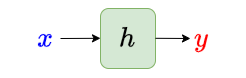
\includegraphics[width=50mm,scale=0.5]{images/regression_images/hypothesis_box.png}
        
            \caption*{Our hypothesis reads an input $x$, and predicts the output $y$.}
        \end{figure}

        \begin{definition}
            A \vocab{hypothesis} is a \gren{function} we use to predict $y$, based on $x$.

            \begin{equation*}
                y = h(x)
            \end{equation*}

            This is also called a \purp{model} in machine learning.
        \end{definition}

        There are many models we could use: this makes it hard to search for a good one.

        \begin{itemize}
            \item One solution is to restrict ourselves to only a certain \orgg{class} of model. 

            Each of these is a different kind of model we could try:

            \begin{equation*}
                h_A(x) = \red{\theta_1} x + \red{\theta_0} 
                \qquad \qquad
                h_B(x) = \blu{\theta_2} x^2 + \blu{\theta_1} x + \blu{\theta_0} 
                \qquad \qquad
                h_C(x) = \grn{\theta_2} \sin (\grn{\theta_1} x) + \grn{\theta_0}
            \end{equation*}
        \end{itemize}

        Each of these formats represents a \purp{hypothesis class}, or a "model class".\\

        \begin{definition}
            A \vocab{hypothesis class} $\mathcal{H}$ is a \purp{set} of possible hypotheses.

            \begin{itemize}
                \item Typically, we include all of the hypotheses with the \gren{same equation format}.
            \end{itemize}
        \end{definition}

        \miniex Let's consider the hypothesis class, represented by $h_A$:
            \note{Not familiar with set notation? $\mathcal{H}_A$ is:
            
            \phantom{}
            
            "the set of every function that looks like $\red{\theta_1} x + \red{\theta_0}$".}

        \begin{equation}
            \mathcal{H}_A = \setty{h(x) \quad : \quad h(x) = \red{\theta_1} x + \red{\theta_0}  }
        \end{equation}

        Here are a few example functions from $\mathcal{H}_A$:

        \begin{equation*}
            \begin{matrix}
                h_1(x) = \red{1}x+\red{5} &&&  h_2(x) = \blu{3}x-\blu{9} &&& h_3(x) = \grn{-10}x+\grn{10} &&& h_4(x) =\org{e^2}x-\org{\pi}
            \end{matrix} 
        \end{equation*}

        This makes things easier: rather than searching all possible hypotheses, we're searching $\mathcal{H}$.\\

        \begin{concept}
            Our goal is to \purp{search} $\mathcal{H}$, to find a good \gren{hypothesis} $h$.
        \end{concept}

        Within a hypothesis class, every hypothesis has the \gren{same structure}.

        \begin{itemize}
            \item What makes a hypothesis different? The \orgg{constants} $\theta_i$.

            \item We call these \vocab{parameters.}\\
        \end{itemize}

        \begin{definition}
            A \vocab{parameter} $\theta_i$ is a \gren{number} that is plugged into the hypothesis.

            \begin{itemize}
                \item Each \purp{hypothesis} $h \in \mathcal{H}$ has a \purp{unique list of parameters} $\Theta$.
            \end{itemize}
        \end{definition}

            \note{Typically, $\theta_i$ is a real number, for our purposes.}

        If we know our model class $\mathcal{H}$, $\Theta$ \gren{fully defines} our hypothesis $h$.

        \begin{figure}[H]
        \centering
            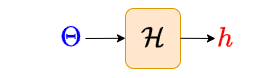
\includegraphics[width=50mm,scale=0.5]{images/regression_images/hypothesis_class.png}
        
            \caption*{By plugging in our $\Theta$ values into the formula for $h$, we get a particular hypothesis.}
        \end{figure}

        For example:

        \begin{figure}[H]
        \centering
            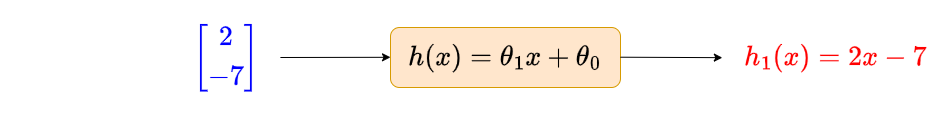
\includegraphics[width=150mm,scale=0.5]{images/regression_images/hypothesis_class_ex.png}
    
        \end{figure}

        This $\Theta$ is what we'll modify, and use to find a \textbf{better model}.\\
        
        \begin{concept}
            Often, we already know which hypothesis class $\mathcal{H}$ we're using.

            \begin{itemize}
                \item So, it's very easy to convert back-and-forth between $\Theta$ and $h$.
            \end{itemize}

            So, we often consider the \purp{parameters} and \gren{hypothesis} interchangeable, or equivalent.

            \begin{itemize}
                \item "Finding a good hypothesis" and "finding good parameters" are, more or less, the same problem.
            \end{itemize}
        \end{concept}

        Notice that we have \orgg{two separate steps} of plugging in, when we use a model $h$:

        \begin{itemize}
            \item When choosing our model $h$, we "plug in" \gren{parameters} $\Theta$ to create our equation.

            \begin{equation}
                h(x) = \grn{\theta_1}x + \grn{\theta_0} 
                \quad \xlongrightarrow{\Theta = \blu{\begin{bmatrix}
                    2 \\ -7
                \end{bmatrix}}} \quad
                h_1(x) = \grn{2}x-\grn{7}
            \end{equation}

            \item When we want to use our model to predict $y$, we "plug in" our \purp{input value} $x$.

            \begin{equation}
                h_1(x) = 2\pur{x}-7 
                \quad \xlongrightarrow{\blu{x=5}} \quad
                h_1(5) = 2(\pur{10})-7 \;\;=13
            \end{equation}
        \end{itemize}

        We'll introduce some new notation to keep the difference clear.\\

        
        
        \begin{notation}
            We can write the same hypothesis $h$ \vocab{two different ways}:

            \begin{equation*}
                h(\red{x}) \qquad \qquad h(\red{x};\blu{\Theta})
            \end{equation*}

            \begin{itemize}
                \item The first notation is denser and \gren{simpler} to read.
                
                \item The second notation includes \purp{$\Theta$}, acknowledging that we had to "plug in" \purp{parameters} to create $h$.
            \end{itemize}

            We \gren{distinguish} between "input variables" and "parameters" by separating them with a \orgg{semicolon} $;$.
        \end{notation}
        
        
        

    \pagebreak
        
    \subsection{The Problem of Regression}
    
        Our hypothesis is a function that solves a \orgg{problem}. What kind of problem are we dealing with?

        We distinguish different types of problems based on two things: 

        \begin{itemize}
            \item \purp{Inputs}: what kind of data do we have to work with?

            \item \gren{Outputs}: what are we trying to predict?
        \end{itemize}

        The notation for functions reflects this idea: what matters most is, "what comes in, and what goes out".
            \note{Functions, of course, weren't specifically designed for machine learning. But the same idea applies to other STEM disciplines.}\\
        
        \begin{notation}
            A \vocab{function} is notated based on what sorts of \gren{inputs} it can take, and the \purp{outputs} it can return. 
            
            A function $f$ is written like this:
            
            \begin{equation*}
                f: \text{set of inputs} \rightarrow \text{set of outputs}
            \end{equation*}
        \end{notation}

        \begin{itemize}
            \item \miniex Suppose that the input is "\orgg{income}" (real number $r \in \RR$) and the output is "\gren{number of hats owned}" (natural number $n \in \NN$). The function for this would be

            \begin{equation*}
                f: \org{\RR} \to \grn{\NN}
            \end{equation*}
        \end{itemize}

        Sometimes, we'll call our set of inputs, the \purp{input space}.\\

        \begin{definition}
            The \vocab{input space} is the set of all \gren{possible inputs} to our hypothesis $h$.
        \end{definition}

            \note{Technically, a \textbf{space} is a set "with \textbf{added} structure", which is about as broad as it sounds.}

        With that out of the way, let's talk about \vocab{regression}:

        \begin{itemize}
            \item In regression, we receive data as a \gren{real-valued vector}, and converting it into a \purp{real number}. 
                \note{Remember the notation for real-numbered vectors we introduced in the last chapter!}
        \end{itemize}
        
        
        Writing this a little more formally:\\
        
        \begin{definition}
            \vocab{Regression} is a \orgg{machine learning problem} where we use a \gren{vector of real numbers} to predict a \purp{real-valued number}.
            
            In other words, we want a \redd{hypothesis} $h$ of the form:
            
            \begin{equation*}
                h: \grn{\RR^d} \rightarrow \pur{\RR}
            \end{equation*}
            
        \end{definition}
        
        \miniex If you have \textbf{3 values} in your input vector (height, weight, age) and \textbf{1 real output} (life expectancy), you would need a hypothesis
        
        \begin{equation*}
            h: \RR^3 \rightarrow \RR
        \end{equation*}
        
        A more visual example:
        
        \begin{figure}[H]
        \centering
            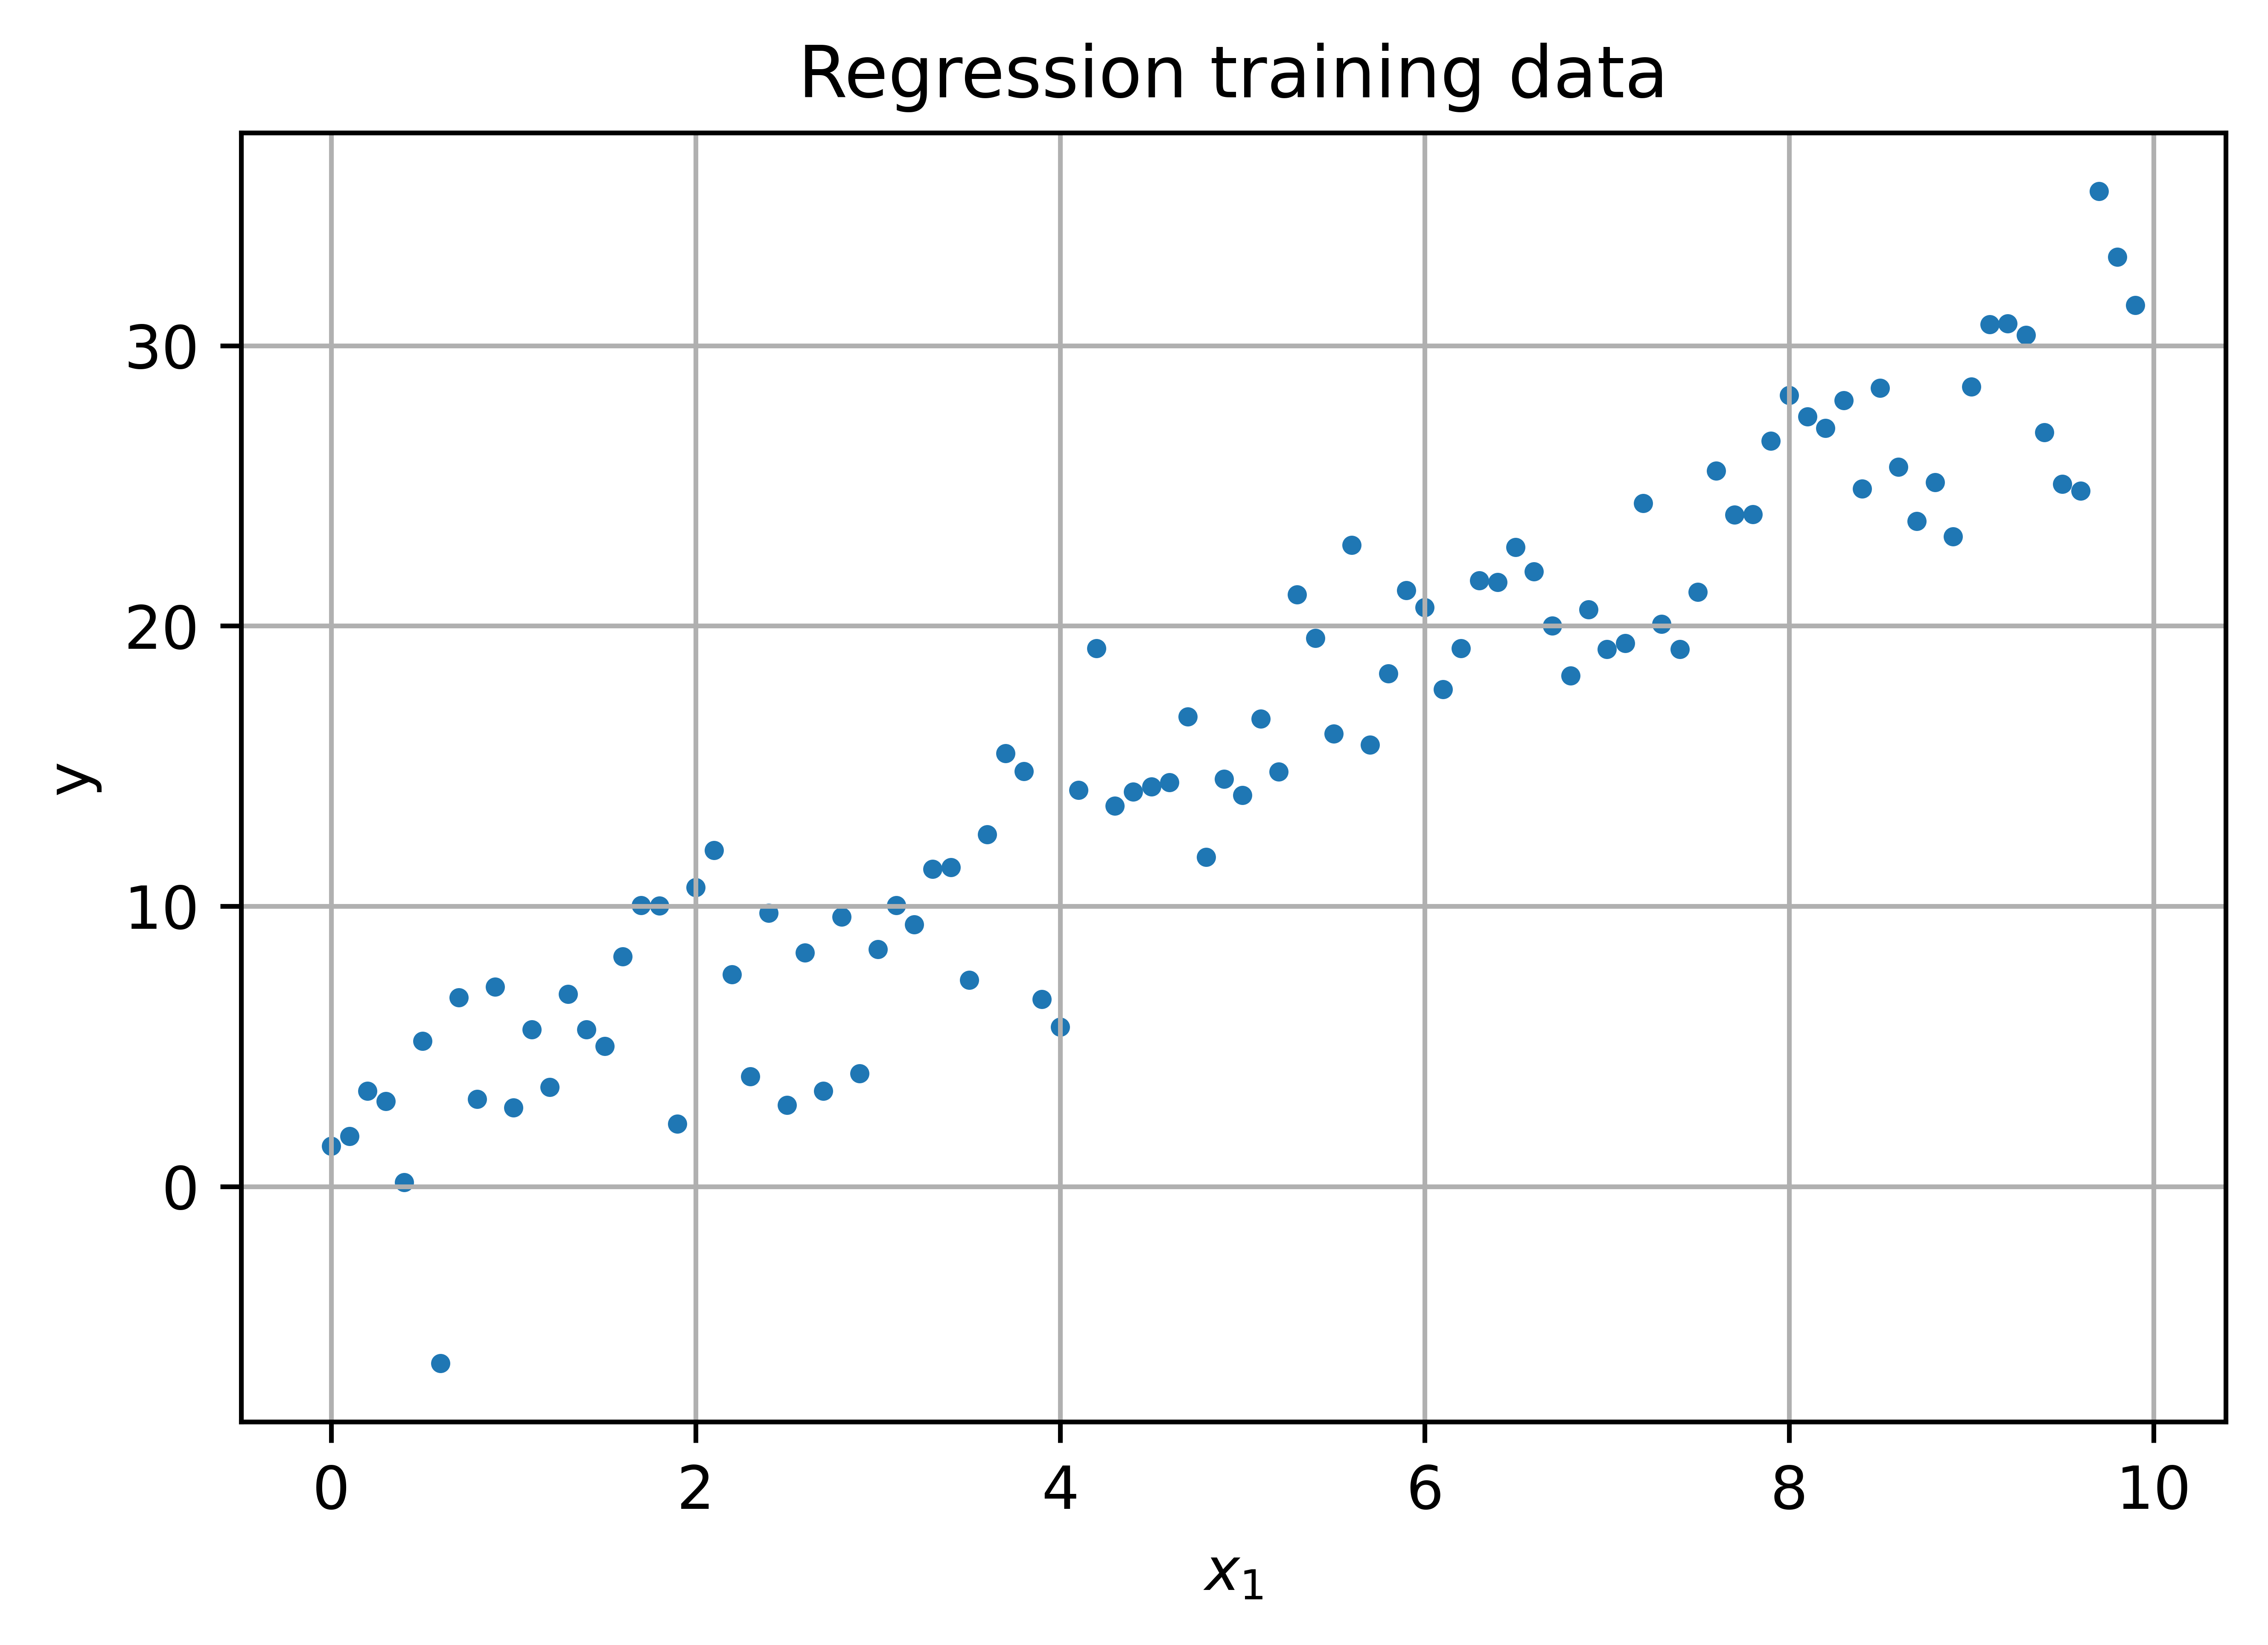
\includegraphics[width=70mm,scale=0.5]{images/regression_images/Regression_Training_Data.png}
        
            \caption*{In this example, you have one input $x \in \RR$ (x-axis), and you want to \textbf{predict} the output $y \in \RR$ (y-axis) based on that. These points are the dataset you want to \textbf{learn} to match.}
        \end{figure}



    \phantom{}
        
    \subsection{Converting our data}
    
        Often, our data \purp{wont fit} this format: maybe we have a car brand, or a color as a variable.

        \begin{itemize}
            \item This requires \gren{converting} this data into real numbers. We do this using something called a \vocab{feature} transformation.\\
        \end{itemize}
        
        
        
        \begin{definition}
            A \vocab{feature} is one distinct piece of \gren{information} in our input.

            \phantom{}
            
            A \vocab{feature transformation} takes those pieces of information, and \purp{transforms} them - often, a more \gren{useful} data type.

            \begin{itemize}
                \item In other cases, we use it on data that's already in the right format, to find \purp{new patterns} in data (we'll return to this idea in a later chapter).
            \end{itemize}
            
        \end{definition}
        
        \miniex You have three car brands. Instead of representing them normally, you instead turn them into vectors: 
        
        \begin{equation}
            \text{Brand A } \to
            \begin{bmatrix}
              1 \\ 0 \\ 0
            \end{bmatrix},
            \;\;\;\;
            \text{Brand B } \to
            \begin{bmatrix}
              0 \\ 1 \\ 0
            \end{bmatrix},
            \;\;\;\;
            \text{Brand C } \to
            \begin{bmatrix}
              0 \\ 0 \\ 1
            \end{bmatrix}
        \end{equation}
        \note{This particular feature transformation is called \textbf{one-hot encoding}! We'll return to it later.}
        
        We do our feature transformation with a function: we often notate this function as $\varphi(x)$.\\

        \begin{notation}
            The \purp{function} we use to do a \vocab{feature transformation} is typically written as $\varphi$.

            \begin{itemize}
                \item If our input data is $x$, the \gren{transformed} data is written as $\varphi(x)$.
            \end{itemize}
        \end{notation}

        \miniex For our above car brand example:

        \begin{equation}
            \varphi\Big(\text{Brand A}\Big) = \begin{bmatrix}
                1 \\ 0 \\ 0
            \end{bmatrix}
        \end{equation}

        There are many different feature transformations for different needs. We will come back to this in a later chapter. 

        \begin{itemize}
            \item For now, we will simply assume that all of our inputs $x$ are \gren{already} in $\RR^d$ (vectors of real numbers).
        \end{itemize}


    \pagebreak
        
        
        
    \subsection{Our dataset}

        Now, we want to find a hypothesis that solves our \textit{particular} regression problem well.

        \begin{itemize}
            \item But in order to predict results, we need \gren{data}.\\
        \end{itemize}

        \begin{concept}
            \vocab{Regression} is a \orgg{supervised problem}:

            This means that, when we're trying to predict the correct answer $y$, we \gren{already have} that answer.

            \begin{itemize}
                \item That way, we can check how good/bad our model's \purp{prediction} was.
            \end{itemize}
        \end{concept}

        \miniex A student practicing "supervised learning" has a practice exam, with all of the solutions.

        \begin{itemize}
            \item They try to do the exam \orgg{without} looking at the solutions.
            \item After they finish, they \gren{check} the solutions, to see what they did wrong, and how they can do better.
        \end{itemize}

        In this analogy, each data point includes a "\gren{question}" (input $x$) and the "\purp{answer}" (output $y$) to that question.

        \begin{figure}[H]
            \centering
            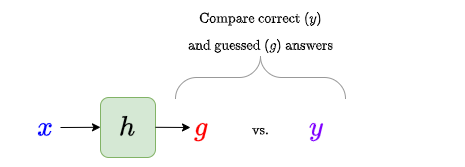
\includegraphics[width=90mm,scale=0.5]{images/regression_images/hypothesis_guess.png}
        
            \caption*{Our model doesn't actually produces $y$: it produces a guess $g$, which we hope is similar to $y$.}
        \end{figure}
        
        We want to \orgg{pair up} inputs with their correct outputs, so we'll write our first data point as 

        \begin{equation}
            \Big(x,y \Big)
        \end{equation}

        But we have many data points we need to sort, like this.

        \begin{itemize}
            \item We'll distinguish each data point using $\ex{x}{i}$ notation, from last chapter:\\
        \end{itemize}

        \begin{notation}
            $x^{(i)}$ is the \vocab{$\nth{i}$ data point}, represented as a vector.

            \begin{itemize}
                \item Sometimes, you may instead see the notation $x_i$.
            \end{itemize}
            
        \end{notation}
        
        We can rewrite this as:
        
        \begin{equation*}
            \left( \ex{x}{1}, \ex{y}{1} \right)
        \end{equation*}
        
        Repeating this for all of our data, we have a set of $n$ data points, $\dataTrain$:
        
        \begin{equation*}
            \dataTrain = 
            \left\{  
            \left(\ex{x}{1}, \ex{y}{1}\right), \dots,
            \left(\ex{x}{n}, \ex{y}{n}\right)
            \right\}
        \end{equation*}

    \phantom{}
        
    \subsection{Training our model}

        We'll use this \purp{training data} to train our model: hopefully, if our model performs well with this limited data, it'll perform well with new data.
            \note{But as we'll see below, that's not always the case.}

        In order to train our model, we need to know how \gren{good} or bad it is, on the data we can see.

        \begin{itemize}
            \item We'll measure the "badness" of our model as \vocab{loss}, from last chapter.\\
        \end{itemize}

        

        \begin{definition}
            \textit{(Review from Introduction Chapter)}
        
            A \vocab{loss function}  measures how \purp{poorly} your machine is \purp{performing} on a \gren{task}.

            \begin{itemize}
                \item The output is a \gren{real number}.
            \end{itemize}
        \end{definition}
        
            \note{If your machine is performing \purp{well}, then you will have a \purp{low} output. And vice versa: if it is doing \gren{badly}, it will have a \gren{high} output.}

        \begin{figure}[H]
            \centering
            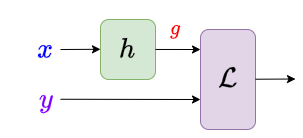
\includegraphics[width=70mm,scale=0.5]{images/regression_images/hypothesis_loss.png}
            \caption*{Our loss function gives us our tool for "comparing" $y$ to $g$.}
        \end{figure}

        We'll take the \purp{average} loss, across all of our \purp{training data}. This is our \vocab{training error}.\\

        \begin{kequation}
        
            \vocab{Training Error} $\trainerr$ is written as:
            
                \begin{equation*}
                    \trainerr(h) \;=\; \red{ \frac{1}{n}  \sum_{i=1}^n } \ex{Loss}{i} \quad=\quad 
                    \frac{1}{n}  \sum_{i=1}^n \loss 
                    \left( \pur{ h(\ex{x}{i}), \; \ex{y}{i} } \right)
                \end{equation*}

            This is the \orgg{expected} (average) loss over all of our training data.
        \end{kequation}

        Note that this is a bit weird: we're using $h$ as an input.

        \begin{itemize}
            \item We want $\trainerr$ to \gren{evaluate} and compare different hypotheses $h$: it has to receive that hypothesis in order to evaluate it.
                \note{The hypothesis, in turn, takes the training data as input.}\\
        \end{itemize}

        \begin{clarification}
            $\vocab{h}$ is a \gren{function} that takes a \gren{variable}, $x$, as its input. This is the usual format.
            
            \vocab{$\trainerr$} is also a function, but it takes in $h$, a \orgg{different function}, as an input!

            \begin{itemize}
                \item That means one function is using \purp{another function} as an input. This can sometimes cause confusion.
            \end{itemize}

            We do this because $\trainerr$ observes our hypothesis, and outputs, "\purp{how bad} in this particular hypothesis at \gren{predicting} this data".
        \end{clarification}

        "Training", in the simplest case, boils down to reducing our error as much as possible.
            \note{Below, we'll add another component, that makes this more complicated.}

            \begin{itemize}
                \item But wait: our goal \purp{isn't} to improve performance on our \gren{training data}. 

                \item Our goal is to perform well on \orgg{new data}!
            \end{itemize}

    \phantom{}
        
    \subsection{Learning to Generalize}
            
        Above, our idea was, "get better at practice data, get better at future data". But this has a problem:

        \begin{itemize}
            \item Even though our training data and future data should be from the \gren{same distribution} (IID), \orgg{randomness} means they won't be exactly the same.
                \note{So if we perfectly matched our training data, we'd be inaccurate to the real distribution.}
        \end{itemize}

        In the last chapter, we introduced a solution: a second dataset, that we \purp{test} our data on.

        \begin{itemize}
            \item We want our machine to handle \gren{new situations} it hasn't seen before: testing data allows us to try out a "new situation".\\
        \end{itemize}

        \begin{definition}
            \vocab{Generalization} is the ability to take something \purp{specific}, and apply it to something more \gren{broad}.

            \begin{itemize}
                \item In machine learning, we want our model to look at some \purp{limited data}, and be able to perform well on a much larger body of \gren{future data} it hasn't seen before.
            \end{itemize}
        \end{definition}
        
        So, let's find out how well our model generalizes. We'll define \vocab{test error}: our performance on the \purp{testing data}. This time, we have $m$ new data points.
        
        \begin{equation}
            \testerr(h) = \frac{1}{\red{m}}  \sum_i  \loss 
            \left( h(\ex{x}{i}), \; \ex{y}{i} \right) 
        \end{equation}
        
        We'll start counting from $n+1$ because we've already used the first $n$ points when training.
            \note{We could start over from $i=1$, but that would be a bit confusing. If you said "the 10th data point", someone might ask, "from the training, or testing data? This avoids this problem.}
        
        \begin{kequation}
        
            \vocab{Testing Error} $\testerr$ is written as:
            
            \begin{equation*}
                \testerr(h) =
                \frac{1}{m}  \sum_{i\purp{=n+1}}^{\purp{n+m}} \loss 
                \left( h(\ex{x}{i}), \; \ex{y}{i} \right) 
            \end{equation*}
        \end{kequation}
        
        
        Because we want to generalize, we want to minimize \textbf{test error}.
        
        \begin{itemize}
            \item But, because we want our model to do well on "data it \gren{hasn't seen} before", we can't use it during our training process.
        \end{itemize}
        
        For now, the next best thing after "minimize test error" is "\vocab{minimize training error}", while using techniques to improve how we \orgg{generalize}. 
            \note{How can we "generalize" if we can't see all of that extra data? We'll get into that below.}

\pagebreak
%%%%%%%%%%%%%%%%%%%%%%%%%%%%%%%%%%%%%%%%%%%%%%%%%%%%%%%%%%%%%%%%%%%%%%%%%%%%%%%%%%%%%%%%%%%

\section{Regression as an optimization problem}
    
    We want to make our \purp{loss} (error) as low as we can: we want to \gren{minimize} it. This is a form of \vocab{optimization} - getting the best results from our system.
        \note{Most of computer science boils down to some kind of optimization.}
    
    Here, we'll introduce some of the terms and notation of optimization.

    \phantom{}
    
    \subsection{Objective Function}

        Now, we confront a major challenge: we have two different priorities.

        \begin{itemize}
            \item We want to perform well on \purp{training data}: our model will learn some insights about the true distribution of data.

            \item But we also want our model to \orgg{generalize} well: we want it to do well data on it has never seen before.
                \note{Because our training data gives us a limited view of the true distribution.}
        \end{itemize}

        Currently, our approach focuses on one priority: we measure our success using \gren{training error}.

        \begin{equation}
            \frac{1}{n}  \sum_{i=1}^n \loss 
                    \left( \pur{ h(\ex{x}{i}), \; \ex{y}{i} } \right)
        \end{equation}

        \begin{itemize}
            \item This function represents "what we consider \gren{important}": it mathematically describes what we want to improve.

            \item We call this an \vocab{objective function}.\\
        \end{itemize}

        \begin{definition}
            An \vocab{objective function} $J$ is the function that tells us what we want to improve, or \purp{optimize}:
            
            \begin{itemize}
                \item Usually, this means that our goal is \gren{minimizing} it.
            \end{itemize}
            
            We minimize our objective function by adjusting our model, via \orgg{parameters} $\Theta$. So, we take that as our input: \purp{J($\Theta$)}.
        \end{definition}

        Since we are focusing more on $\Theta$ then before, we'll replace $h(\ex{x}{i})$ with \blu{$h(\ex{x}{i}; \Theta)$}:
        
        \begin{equation*}
            J(\Theta) = \text{Training Error} = 
            \frac{1}{n}  \sum_{i=1}^n \loss \Big( h(\ex{x}{i}; \blu{\Theta}), \ex{y}{i} \Big) 
        \end{equation*}

    \subsection{The Regularizer}

        If our objective function describes "what we care about", and we care about \gren{generalization}, shouldn't we \purp{include} it in our objective function?

        \begin{itemize}
            \item Let's do that: we'll call it a \redd{regularizer} term.
        \end{itemize}

        \begin{equation}
            J(\Theta) = \text{Training Error} + \red{\text{Regularizer}}
        \end{equation}

        We continue using our training error from before:

        \begin{equation}
            J(\Theta) = \frac{1}{n}  \sum_{i=1}^n \loss 
                    \left( \pur{ h(\ex{x}{i}; \Theta), \; \ex{y}{i} } \right) + \red{\text{Regularizer}}
        \end{equation}

        Later, we'll construct our regularizer so that minimizing it will create a \gren{more general} model $\Theta$. 

        \begin{itemize}
            \item Because we want to make $\Theta$ more \gren{general}, we'll use it in our regularizer: we'll call it \red{$R(\Theta)$}.
                \note{Our strategy is to \gren{minimize} $J(\Theta)$: by reducing training loss and $R(\Theta)$, we hope to make a better model.}
        \end{itemize}

        \begin{equation}
            J(\Theta) = \frac{1}{n}  \sum_{i=1}^n \loss 
                    \left( \pur{ h(\ex{x}{i}; \Theta), \; \ex{y}{i} } \right) + \red{R(\Theta)}
        \end{equation}

        We're missing one thing: how much do we want to prioritize \red{$R(\Theta)$}, compared to \purp{training error}?

        \begin{itemize}
            \item We'll \vocab{scale} our regularizer by a \gren{constant} $\lambda \geq 0$.

            \item The larger $\lambda$ is, the more we care about \orgg{generalizing} to new data.\\
        \end{itemize}

        \begin{kequation}
            
            In general, we write the \vocab{objective function} as:
            
            \begin{equation*}
                J(\Theta) =
                \left( 
                \frac{1}{n}  \sum_{i=1}^n \loss \Big( h(\ex{x}{i}; \Theta), \;\; \ex{y}{i} \Big) 
                \right)
                +
                \blu{\lambda} \red{ R(\Theta)}
            \end{equation*}

            \begin{itemize}
                \item The left term is the \purp{loss}: how well we perform on training data.
                \item The right term is the \orgg{regularization}: we hope that \gren{minimizing} it will make our model more "general" (good for new situations).
            \end{itemize}
        \end{kequation}

        This is the function we want to \gren{minimize}. What does our \redd{regularizer} look like? 

        

        \begin{itemize}
            \item We'll come back to this later. we'll go one step at a time, and first learn how to minimize \purp{training error}.
        \end{itemize}

    \subsection{More on the Objective Function}

        Notice that our objective function \gren{depends} on our training data $\data$ as well: the same model will work better for some problems, than others.
    
        \begin{itemize}
            \item \miniex A model trained in political science learns different things compared to one trained in geology.
            \item We'd expect it to perform pretty badly on a geology exam.
        \end{itemize}
    
        "$\data$ affects $J$, but isn't the main input" is \gren{similar} to our previous idea: "$\Theta$ affects hypothesis $h$, but we usually \purp{don't} think of it as the \purp{input}".
        
        \begin{itemize}
            \item We made this distinction with some \orgg{notation}: $h(x;\Theta)$.\\
        \end{itemize}
    
        \begin{notation}
            Just like how we can use ";" when writing $h(x;\Theta)$, we'll use the \orgg{same notation} for $J$: $J(\Theta;\grn{\data})$
    
            \begin{equation*}
                    J(\Theta; \grn{\data}) =
                    \left( 
                    \frac{1}{n}  \sum_{i=1}^n \loss \Big( h(\ex{x}{i}; \Theta), \;\; \ex{y}{i} \Big) 
                    \right)
                    +
                    \blu{\lambda} \red{ R(\Theta)}
                \end{equation*}
    
            $\Theta$ is our "main" input variable, but data $\data$ is important for computing $J$.
        \end{notation}

        One more comment:\\

        \begin{clarification}
           Students often get confused by the fact that our \purp{objective function} $J$ is a function of $\Theta$, while \orgg{training error} $\trainerr$ is a function of $h$.

           \begin{equation*}
               \overbrace{
                    J(\Theta)}^{\text{Uses } \Theta} 
                =
                \overbrace{
                    \trainerr(h)}^{\text{Uses } h} 
                + \lambda R(\Theta)
           \end{equation*}
            
            The difference is that \orgg{training error} $\trainerr(h)$ is \gren{more general} than the \purp{objective function} $J(\Theta)$, and \orgg{$h$} is \gren{more general} than \purp{$\Theta$}.

            \begin{itemize}
                \item By "more general", we mean that there are more situations where we can use $h$ than $\Theta$.
                \begin{itemize}
                    \item $\Theta$ is a list of parameters: we only use it if we have a \purp{parametric model}.
                    \item $h$ is used if we have \orgg{any kind of model}.
                \end{itemize}
            \end{itemize}

            
            So, let's compare $\trainerr(h)$ and $J(\Theta)$:
            
            \begin{itemize}
                \item \orgg{Training error} 
                can be used for any model $h$, so we don't want to use $\Theta$: our model could be \gren{non-parametric}.
                
                \item Our \purp{objective function} \gren{assumes} we have parameters $\Theta$: we know our model class $H$, we just want to optimize $\Theta$.
            \end{itemize}
            
        \end{clarification}
        
    \pagebreak
        
        
        
        
        
        
    \subsection{Minimization Notation}
        
        Our goal is to \gren{minimize} $J$ by adjusting $\Theta$. To demonstrate, we'll use the following example:

        \begin{figure}[H]
            \centering
            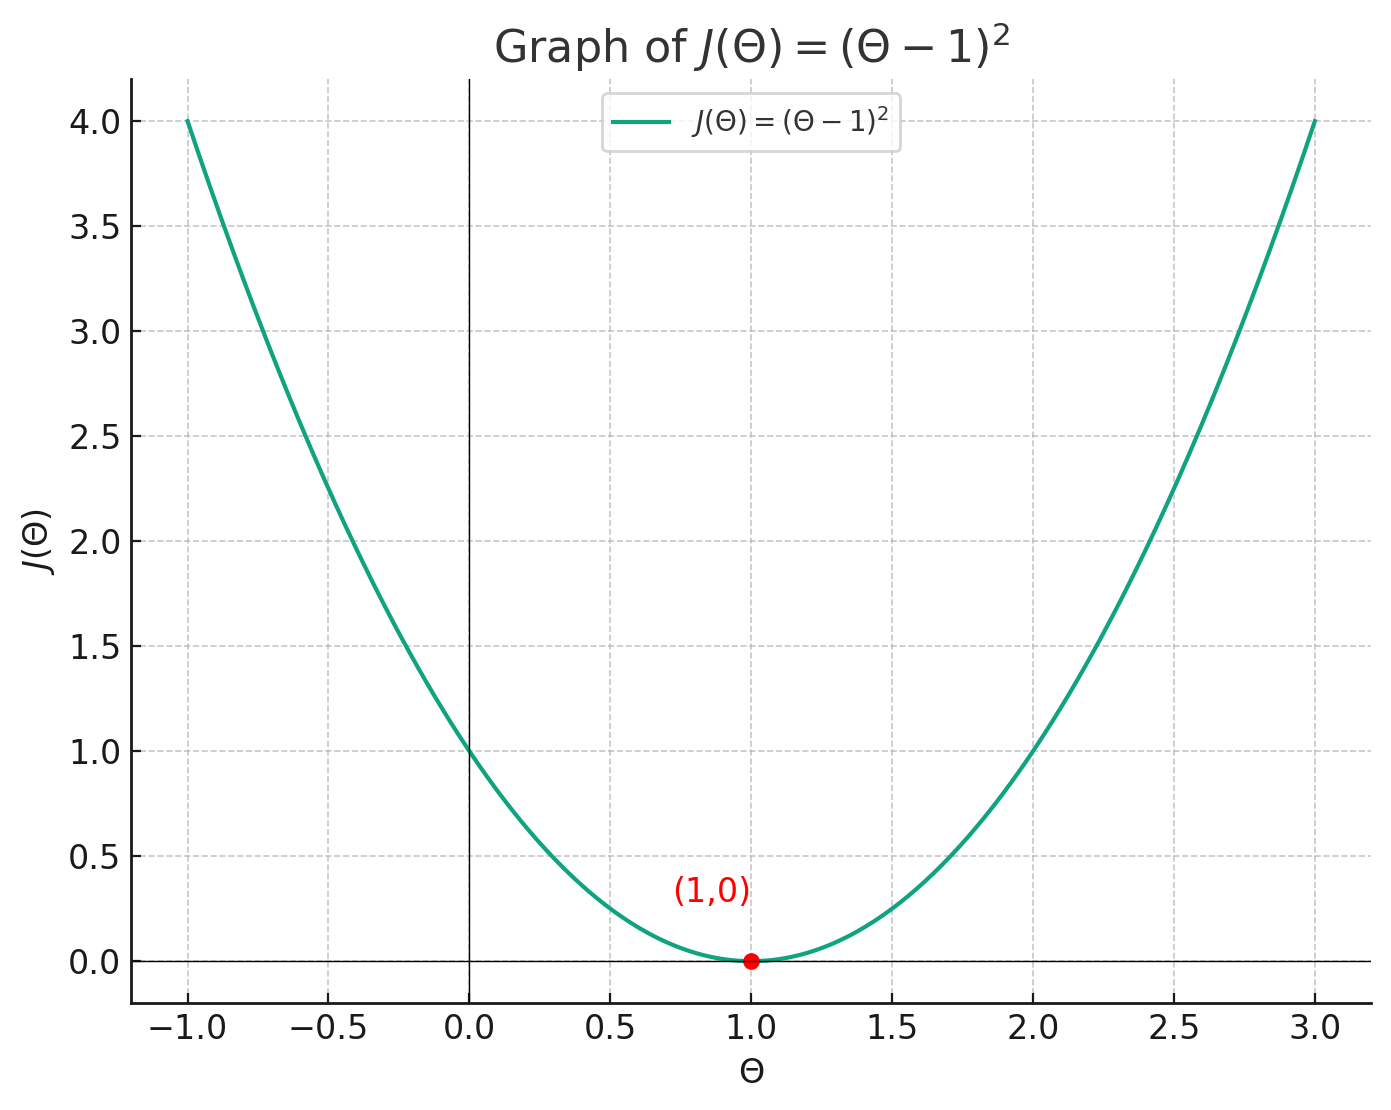
\includegraphics[width=70mm,scale=0.5]{images/regression_images/minimizing_(x-q)^2.png}
        
            \caption*{Take $J(\Theta)=(\Theta-1)^2$. The minimum output is 0, which happens at $\Theta=1$. So, we have a minimum at $(1, 0)$.}
        \end{figure}

        Our goal is to find this \vocab{minima}. There are two questions we're interested in:

        \begin{itemize}
            \item What is the \purp{minimum value of $J$} we can find by \orgg{adjusting $\Theta$}?
            \item Which \gren{model $\Theta$} gives us the minimal $J$? In other words: which model performs best?
        \end{itemize}

        We define a distinct function for answering each of these questions. 
        
        \phantom{}
        
        First:
        
        \begin{itemize}
            \item What is the \purp{minimum value of $J$} we can find by \orgg{adjusting $\Theta$}?\\
        \end{itemize}
        
        \begin{notation}
            The \vocab{min function} gives you the \gren{minimum output} of a function we get by adjusting one chosen \purp{variable}.
            
            \begin{equation*}
                \min_{ \pur{ \Theta } }{ \grn{ J(\Theta) } }
            \end{equation*}
            
            The \gren{function we want to minimize} is written to the right, while the \purp{variable we adjust} is written below.
        
        \end{notation}
        
        \miniex 
        
        \begin{equation}
            \min_{\Theta}{ \red{(\Theta-1)^2} } = \red{0}
        \end{equation}

        0 is the minimum value of $J$ we can find by adjusting $\Theta$.

        \phantom{}

        Next:
        
        \begin{itemize}
            \item What is the \purp{minimum value of $J$} we can find by \orgg{adjusting $\Theta$}?\\
        \end{itemize}
        
        \begin{notation}
            The \vocab{argmin function} tells you the value of the \purp{input variable} that gives the \gren{minimum output}.
            
            \begin{equation*}
                \argmin{ \pur{ \Theta } }{ \grn{ J(\Theta) } }
            \end{equation*}
            
            The \gren{function we want to minimize} is written to the right, while the \purp{variable we adjust} is written below.
        
        \end{notation}
        
        \miniex
        
        \begin{equation}
            \argmin{\red{\Theta}}{ (\Theta-1)^2 } = \red{1}
        \end{equation}

        1 is the value of $\Theta$ which gives the minimum $J$.\\

        \begin{clarification}
            Why is it called "\vocab{argmin}"?

            "\gren{Argument}" is used as another word for "\gren{input variable}".

            And our argmin function returns the \gren{argument} with the \purp{minimum} output. Hence, \gren{arg} \purp{min}.
        \end{clarification}
        
          

        

        \phantom{}
        
    \subsection{Optimal Value Notation}
        
        Our goal is to find the best model, represented by some $\Theta$. We'll call this "optimal" model, $\Theta^*$.\\
        
        \begin{notation}
            We add a \vocab{star} $^*$ to indicate the \purp{optimal} variable choice.
            
            If that variable is $z^*$, you would say it as "$z$-star".
        \end{notation}
        
        \miniex 
        
        \begin{equation}
            \Theta^* = 1 \text{ for the above example.}
        \end{equation}
        
        So, if we want optimal $\Theta$, we're looking for:\\
        
        \begin{kequation}
        
            Our \vocab{optimal parameter} vector is written as 
            
            \begin{equation*}
                \Theta^* = \argmin{ \Theta  }{  J(\Theta)  }
            \end{equation*}
        \end{kequation}
        


\pagebreak
%%%%%%%%%%%%%%%%%%%%%%%%%%%%%%%%%%%%%%%%%%%%%%%%%%%%%%%%%%%%%%%%%%%%%%%%%%%%%%%%%%%%%%%%%%%

\section{Linear Regression}

    Now that we understand the problem of \gren{regression}, and the concept of \purp{optimizing} over it, we'll introduce our \orgg{hypothesis class.}
    
    We want a function that can use information to \gren{predict} outputs.
    
    \subsection{The Linear Model, 1-D}
    
        We'll start off small: we have \gren{one variable}, and something we want to predict. And we'll pick the simplest pattern we can:

        \begin{equation}
            y = mx+b
        \end{equation}
        
        A \vocab{linear} equation.
        
        \begin{itemize}
            \item $m$ tells us \textbf{how much} our input $x$ \gren{affects} our output $y$.
            \item $b$ accounts for everything \purp{unrelated} to $x$: what is $y$ when $x=0$?
        \end{itemize}

        $b$ and $m$ are our \orgg{parameters}: that means they're part of $\Theta$. We'll rename them $b=\theta_0$ and $m=\theta_1$.\\
        
        \begin{equation}
            h(x) = \red{\theta_1} x + \blu{\theta_0}
        \end{equation}

        \begin{figure}[H]
            \centering
            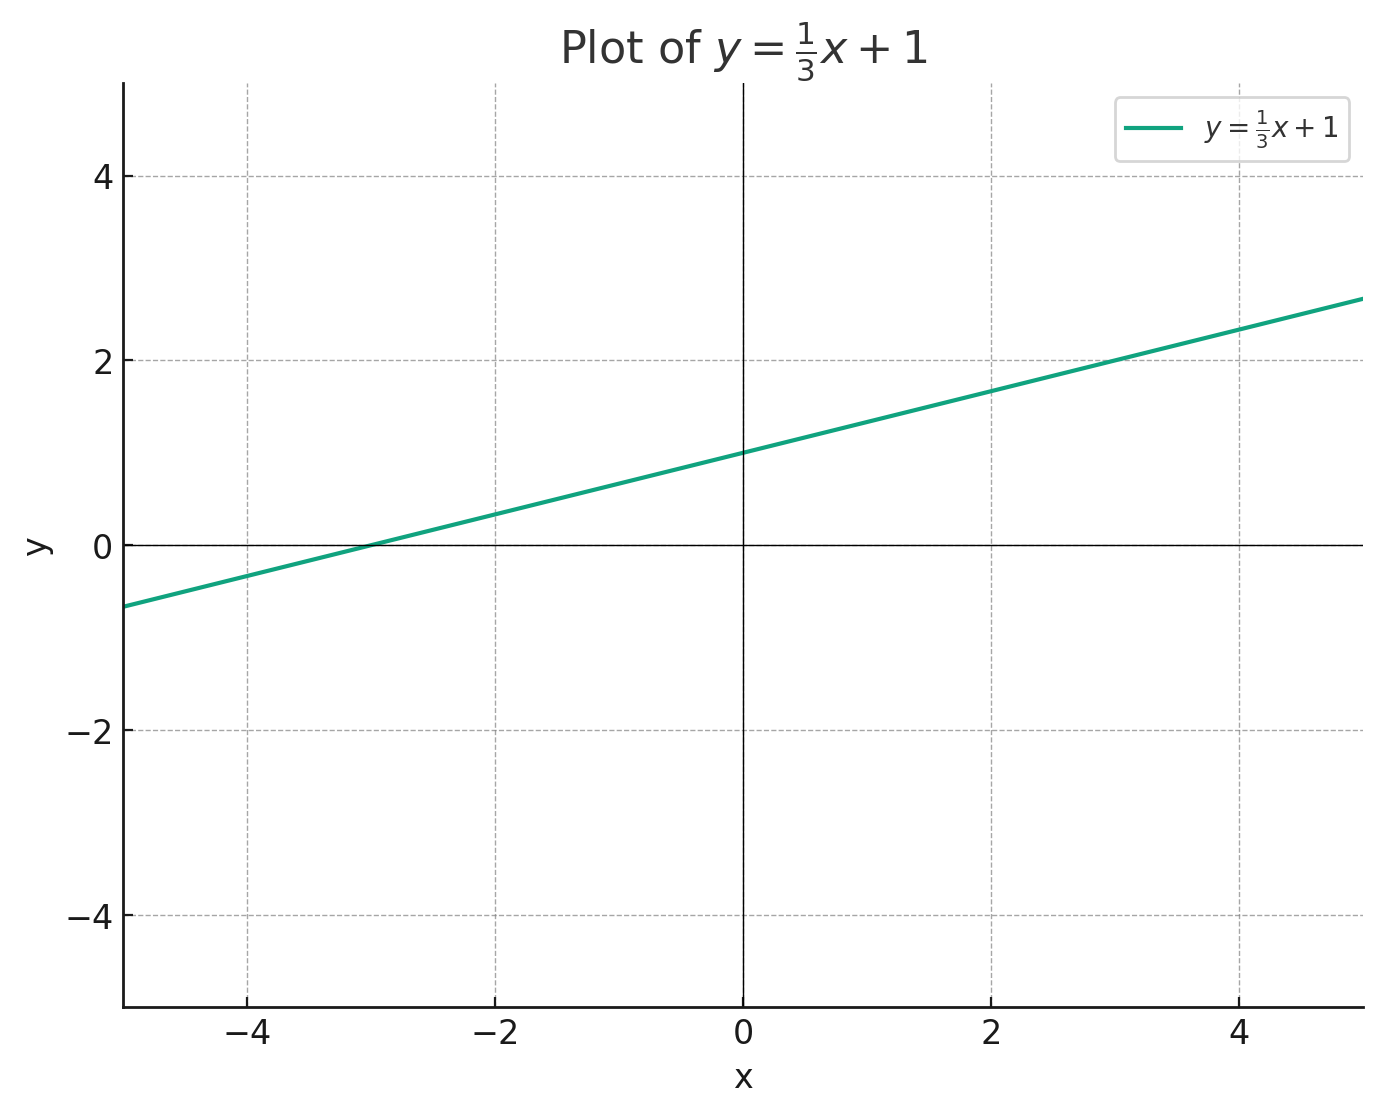
\includegraphics[width=50mm,scale=0.5]{images/regression_images/xover3+1.png}
        
            \caption*{Here's $\frac{1}{3}x+1$. We call this 1D because there's only one input dimension, $x$. But we plot it in 2D to see the output, too!}
        \end{figure}

    \phantom{}
        
    \subsection{The Linear Model, 2-D}
    
        We want to have \textbf{multiple} input variables: $x$ will be a \purp{vector}, not a number. 

        \begin{equation}
            x = \begin{bmatrix}
                x_1 \\ x_2
            \end{bmatrix}
        \end{equation}
        
        So, for our above example, we'll \textbf{replace} $x$ with $x_1$.
        
        \begin{equation}
            h(x) = \theta_1 \red{x_1} + \theta_0
        \end{equation}
        
        The simplest way to include $x_2$ by just \textbf{adding} it. We have a scaling factor $\theta_1$ for $x_1$, so we'll give $x_2$ its own \gren{parameter}, $\theta_2$:
        \note{If $\theta_1$ is the "slope" for $x_1$, $\theta_2$ is the "slope" for $x_2$.}
        
        \begin{equation}
            h(x) = \red{\theta_2 x_2} + \theta_1 x_1 + \theta_0
        \end{equation}

        \begin{figure}[H]
            \centering
            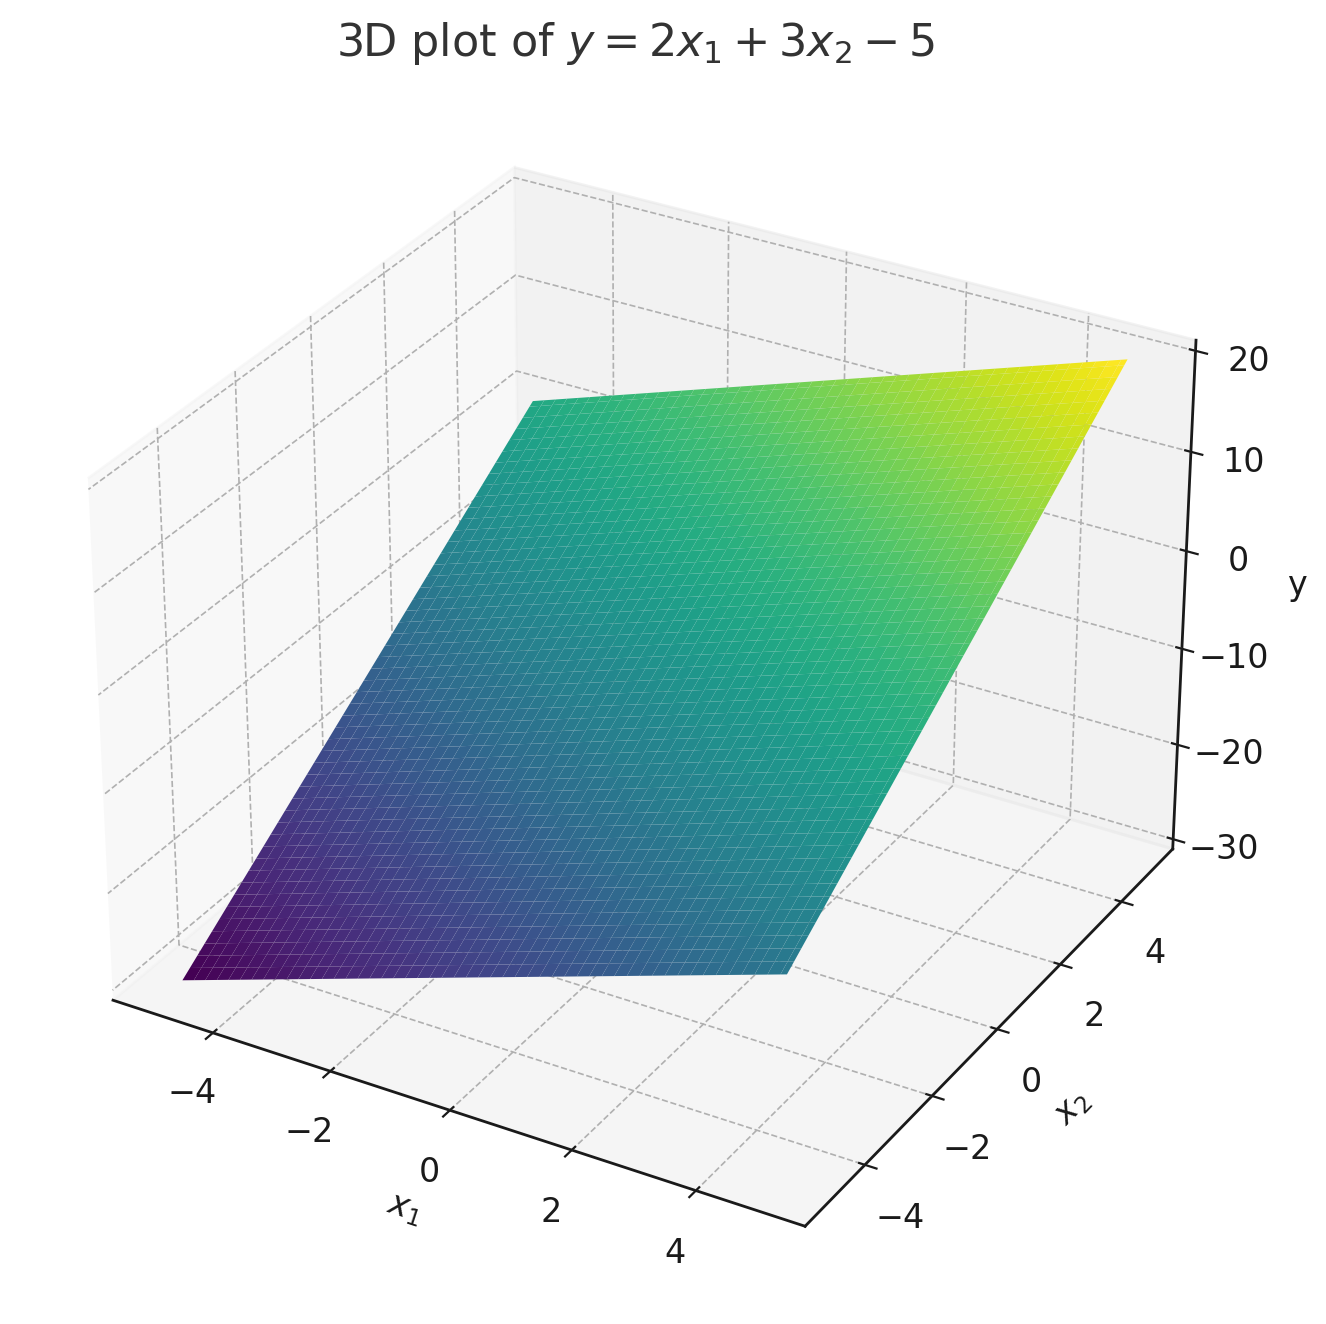
\includegraphics[width=50mm,scale=0.5]{images/regression_images/plane.png}
        
            \caption*{Here's a 2d regression: it's a plane. The height represents the output.}
        \end{figure}
        
    \subsection{The Linear Model, $d$-D}
    
        You can \textbf{expand} this to $d$ dimensions by \purp{adding more terms}:
        \note{This is the "dimension" of our input space: the \textbf{number} of input variables we have.}
        
        \begin{equation}
            h(x) = \blu{\theta_0} + \red{\theta_1}x_1 + \red{\theta_2}x_2 + \red{\theta_3}x_3 + ... + \red{\theta_d}x_d
        \end{equation}

        We need $n+1$ dimensions to plot an $n$-dim regression, so... we can't plot $n>2$.

    \phantom{}
        
    \subsection{The Linear Model using Vectors}
        
        We \textbf{multiply} components of $x$ and $\theta$ together, then \textbf{add} them together. This looks like a \orgg{dot product}:
        
        \begin{equation}
            h(x) = \theta_0 +
            \red{
                \begin{bmatrix}
                    \theta_1 \\ \theta_2 \\ \vdots \\ \theta_d
                \end{bmatrix}
                }
                \cdot
                \blu{
                \begin{bmatrix}
                    x_1 \\ x_2 \\ \vdots \\ x_d
                \end{bmatrix}
            }
        \end{equation}
        
        If we write this symbolically, we get:
        
        \begin{equation}
            h(x) = \theta_0 + \red{\theta} \cdot \blu{x} 
        \end{equation}
        
        $\theta$ includes all of our parameters, \orgg{except for} $\theta_0$.
        
        \begin{itemize}
            \item $\theta$ is used for our \textbf{dot product}, $\Theta$ includes \textbf{all} parameters.\\
        \end{itemize}
        
        \begin{notation}
            We represent the \gren{parameters} of our \purp{linear} equation as $\Theta = (\theta, \theta_0)$.
        \end{notation}
        
        This formula looks similar to $y=mx+b$ again! Only this time, we have \textbf{vectors} instead.
        
        We'll swap out the dot product for \purp{matrix multiplication}.\\

        \begin{kequation}
            A dot product $a \cdot b$ can be written as \vocab{matrix multiplication} instead:

            \begin{equation*}
                a \cdot b = a^Tb
            \end{equation*}
        \end{kequation}
        
        In this class, we'll usually find it more useful to work with matrix multiplication.\\
        
        \begin{definition}
            The \vocab{linear regression} hypothesis is  $h(x)=\theta \cdot x+\theta_0$, or
            
            \begin{equation*}
                h(x) = \red{ \theta^T x } + \theta_0
            \end{equation*}
        \end{definition}
        
        \note{Make sure you know what $\theta^T$ is: it's the \textbf{transpose} of $\theta$.}
        
        Remember that, when written out, this looks like:
        
        \begin{equation}
            h(x) = 
            \red{
                \begin{bmatrix}
                    \theta_1 & \theta_2 & \theta_3 & \cdots & \theta_d
                \end{bmatrix}
            }
            \blu{
                \begin{bmatrix}
                    x_1 \\ x_2 \\ x_3 \\ \vdots \\ x_d
                \end{bmatrix}
            }
            + \theta_0
        \end{equation}
        
        This is the \vocab{hypothesis class} of \textbf{linear hypotheses} we will reuse throughout the class.

    \pagebreak
        
    \subsection{Regression Loss}
    
        We need to decide on our \vocab{loss function} for regression: how \purp{badly} is our model is performing?

        \begin{itemize}
            \item Our goal is for our \purp{guess} $g$ to be close to the \gren{real} output $y$. 

            \item The more \orgg{different} they are, the worse.
        \end{itemize}

        We could use "absolute difference" $|g-y|$, but \vocab{squared difference} tends to be much more useful:
            \note{Why? We discuss in the Concept box below.}
        
        \begin{equation}
            \loss(g,y) = (g-y)^2
        \end{equation}
        
        We call this \vocab{square loss}. It punishes high and low guesses equally, and the punishments become more \textbf{severe} as the \textbf{difference} increases.
        \note{Our slope $\deriv{}{x} x^2 = 2x$ gets larger as we move away from $x=0$.}\\

        \begin{concept}
             We use \vocab{square distance} for a few good reasons:
        
        \begin{itemize}
            \item High and low guesses are treated \purp{equally}.
            
            \item It works well with \orgg{matrix multiplication}:

                \begin{equation*}
                    ||w||^2 = w^Tw
                \end{equation*}
            
            \item $\norm{w}$ is \gren{not smooth}: it doesn't always have a derivative! $\norm{w}^2$ \textit{is} smooth.
                \begin{itemize}
                    \item $\norm{w}$ doesn't have a derivative at $w=0$.
                \end{itemize}

            \item The \orgg{slope} becomes \orgg{small} when you get closer to the correct answer: you'll know when you're getting close.
        \end{itemize}
        \end{concept}

            \note{A "stronger" version of smoothness requires that \gren{every derivative} ($f'$, $f''$, $f'''$...) is \gren{continuous}.
            
            \phantom{}
            
            We just care if the derivative exists everywhere, though.}

        \begin{figure}[H]
            \centering
            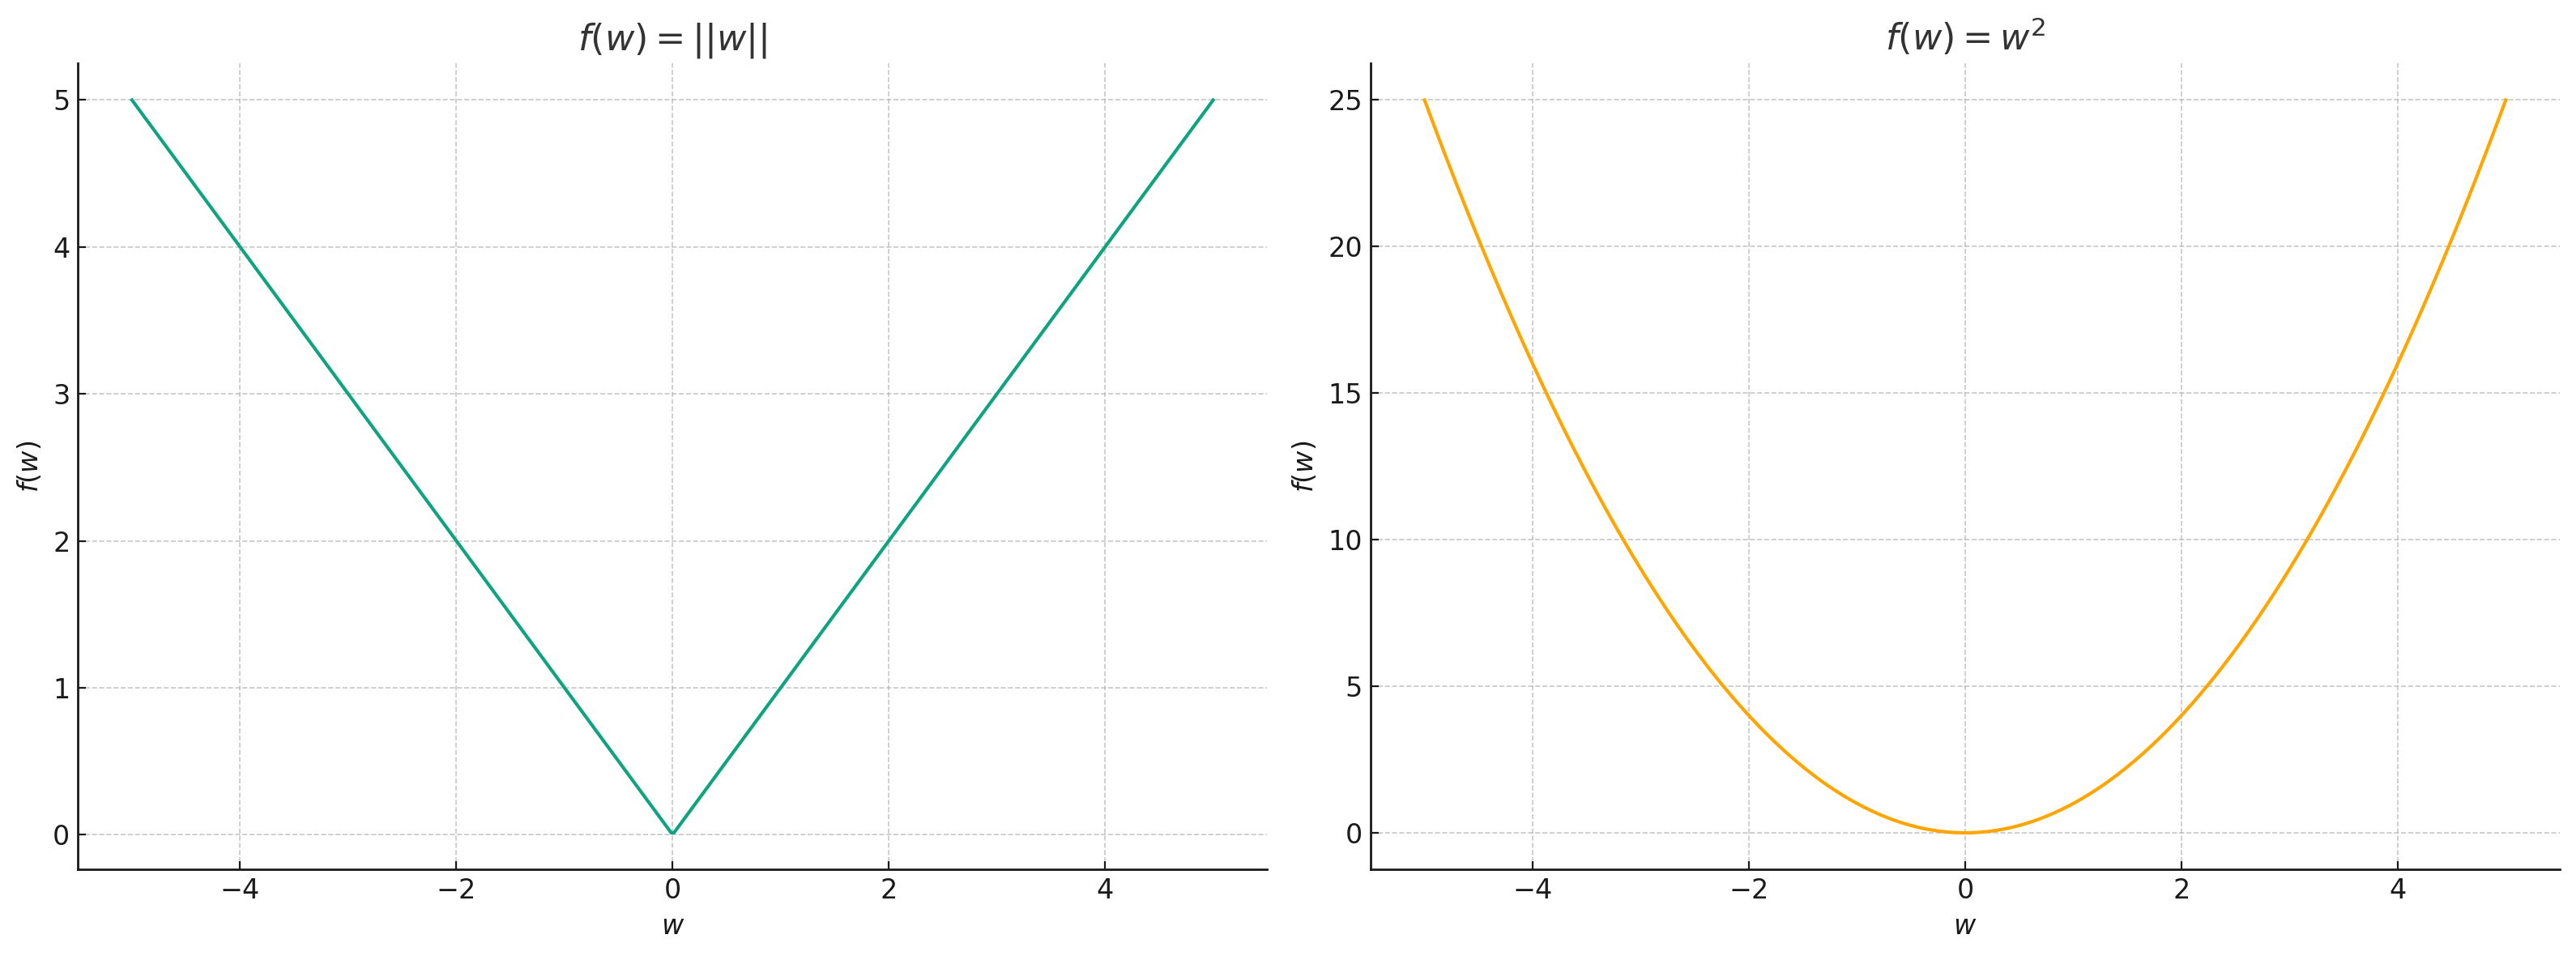
\includegraphics[width=100mm,scale=0.5]{images/regression_images/abs_w_vs_w_squared.png}
        
            \caption*{What's the derivative of $||w||$ at 0? We don't have one!}
        \end{figure}

        
        
    \phantom{}
        
    \subsection{Our Goal: Ordinary Least Squares}

        Now, we have the concepts we need.

        \begin{itemize}
            \item We want to \purp{minimize} loss $\loss$ on our data set, using the \gren{linear} model $\Theta$ ($h$).

            \item We'll use that linear model to \orgg{predict} the outputs of our data points.
        \end{itemize}
        
        This goal can be turned into an \purp{objective function}: $J(\Theta)=J(\theta,\theta_0)$
        
        \begin{equation}
            J(\theta,\theta_0) = \text{\pur{Training Loss}}
        \end{equation}

        Let's go step-by-step:

        \begin{itemize}
            \item Training loss is our \purp{expected loss}, averaged over each data point. $\red{\ex{g}{i}}$ is our prediction for $\blu{\ex{y}{i}}$.
            \note{Remember that $\blu{\ex{y}{i}}$ is the "correct" answer for our \grn{$\nth{i}$ data point}.}
        
        \begin{equation}
            J(\theta,\theta_0) = 
            \frac{1}{n}  \sum_{i=1}^n 
            \pur{\loss} ( \ex{g}{i},  \ex{y}{i}  )
        \end{equation}

            \item We'll use \gren{squared loss} to evaluate each data point:
        
        \begin{equation}
            J(\theta,\theta_0) = 
            \frac{1}{n}  \sum_{i=1}^n 
            \Big( \red{\ex{g}{i}}  - \blu{\ex{y}{i}} \Big)^{\grn{2}}
        \end{equation}

            \item We use our \textbf{hypothesis} $\red{h(} \blu{\ex{x}{i}} \red{;\Theta)}$ to make our guess $\red{\ex{g}{i}}$.
        
        \begin{equation}
            J(\theta,\theta_0) = 
            \frac{1}{n}  \sum_{i=1}^n 
            \left( 
                \red{h(} \blu{\ex{x}{i}} \red{;\Theta)} -  \ex{y}{i} 
            \right)^2 
        \end{equation}

            \item Our hypothesis is a \orgg{linear model} $\theta^T \blu{\ex{x}{i}}  + \theta_0$.\\
        \end{itemize}

        
        
        
        \begin{kequation}
            The \vocab{ordinary least squares} \vocab{objective function} for \purp{linear regression} is written as 
            \begin{equation*}
                J(\theta,\theta_0) = 
                \frac{1}{n}  \sum_{i=1}^n 
                \left( \red{ (\theta^T} \blu{\ex{x}{i}} \red{ + \theta_0) } 
                \quad-\quad \blu{\ex{y}{i}} \right)^2 
            \end{equation*}
        \end{kequation}
        
        If we break this into parts:
        
        \begin{equation}
            J(\theta,\theta_0) = 
                        \underbrace{
                            \frac{1}{n}  \sum_{i=1}^n 
                        }_{Averaging}
                        \left( 
                            \underbrace{
                                \red{ (\theta^T} \blu{\ex{x}{i}} \red{ + \theta_0) } 
                            }_{guess}
                            \quad-\quad 
                            \underbrace{
                                \blu{\ex{y}{i}}
                            }_{answer}
                        \right)^2 
        \end{equation}
        
        Now, this is an \purp{optimization} problem. We need to find the model $(\theta, \theta_0)$, that gives us the best (minimal) $J$.
            \note{We now have two parameters in our argmin function, but aside from listing both of them, the notation is the same. We just substituted $\Theta = (\theta, \theta_0)$}
        
        \begin{equation*}
            \theta^*, \theta_0^* = \argmin{\theta, \theta_0}{J(\theta,\theta_0)}
        \end{equation*}

        \phantom{}
        
    \subsection{Visualizing our Model}
    
        We'll start with the \vocab{one-variable} case. With one input, one output, we use a 2D plot to graph our data.

        \begin{itemize}
            \item Each piece of data is a simple $(x,y)$ pair: a \purp{point}.

            \item Meanwhile, our hypothesis is a \gren{line}: for each $x$, it predicts a different $y$.
        \end{itemize}
        
        \begin{figure}[H]
        \centering
            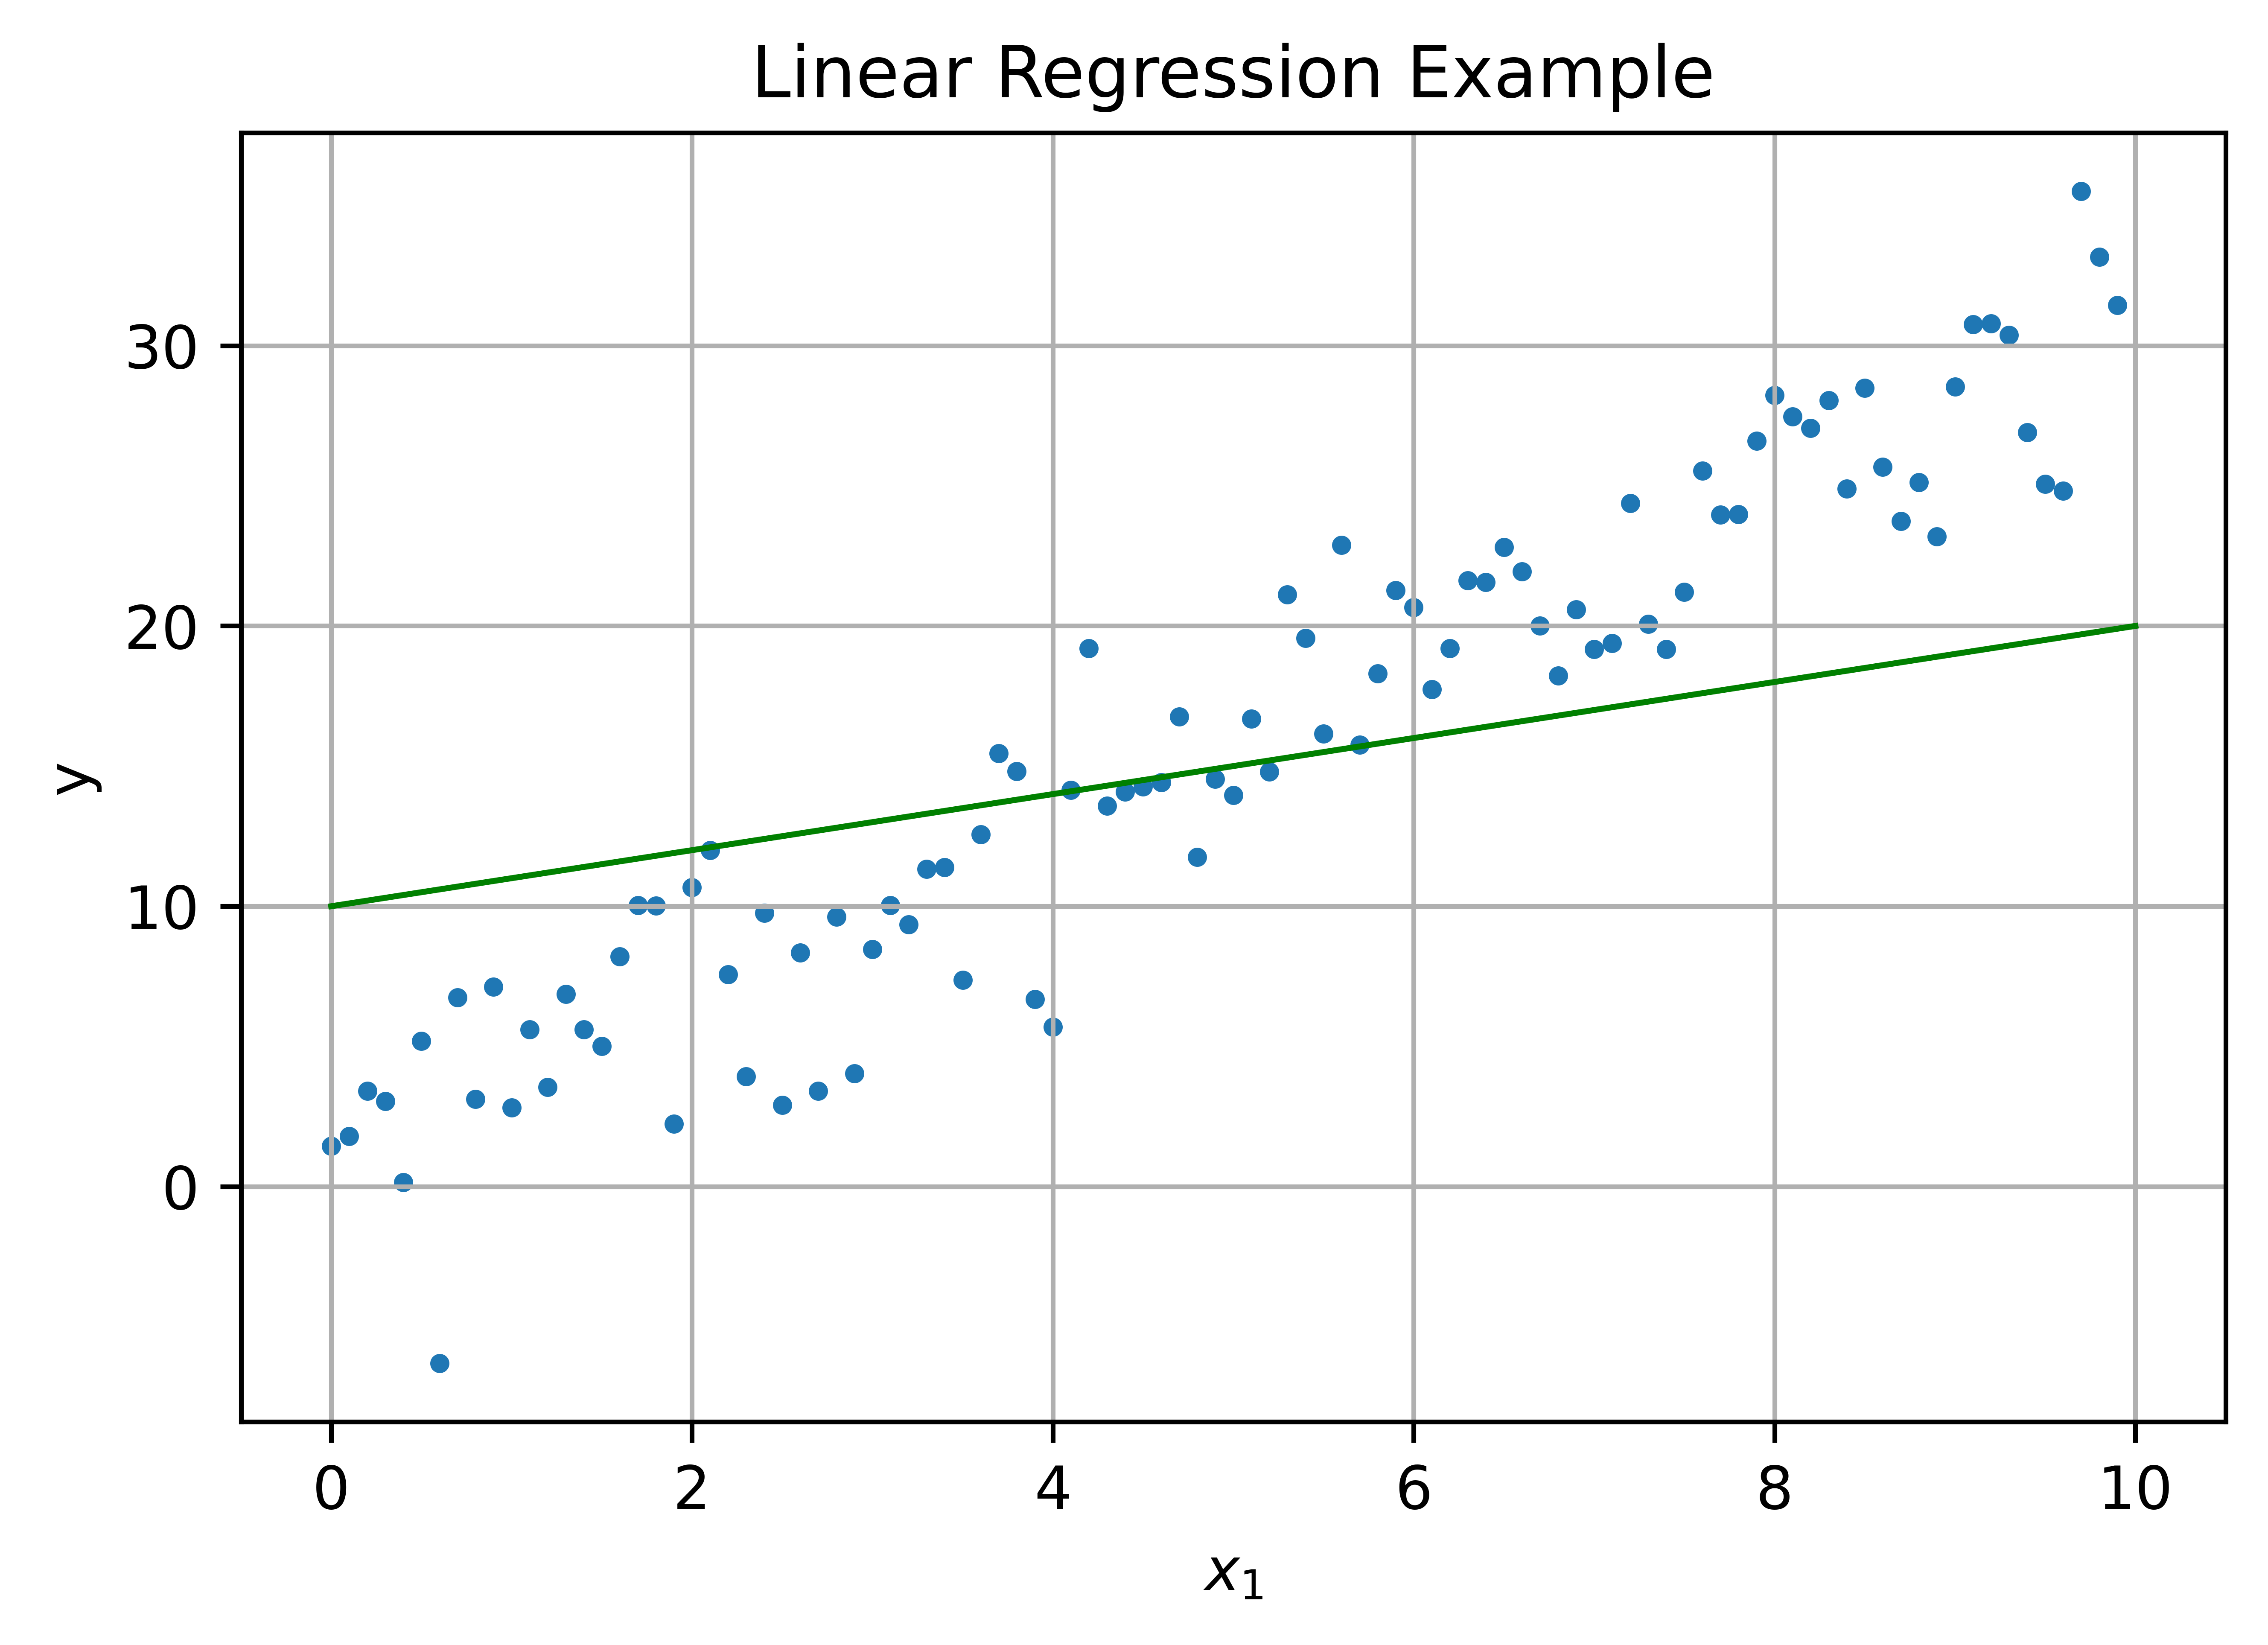
\includegraphics[width=70mm,scale=0.5]{images/regression_images/Regression_Example_Poor_Fit.png}
        
            \caption*{This linear model doesn't fit our data very well: $(\theta_0=10, \theta_1=1)$}
        \end{figure}

            \note{How do we know our line doesn't fit our data? Because it isn't "close" to the shape of the data.
            
            \phantom{}
            
            We want our model to really represent the data it comes from: they should look similar.}
        
        We're trying to get our line as \purp{close as possible} to the points, hoping to find a linear pattern. 
        
        \begin{itemize}
            \item We call this "\orgg{fitting}" our line to the data.
        \end{itemize}
        
        \begin{figure}[H]
        \centering
            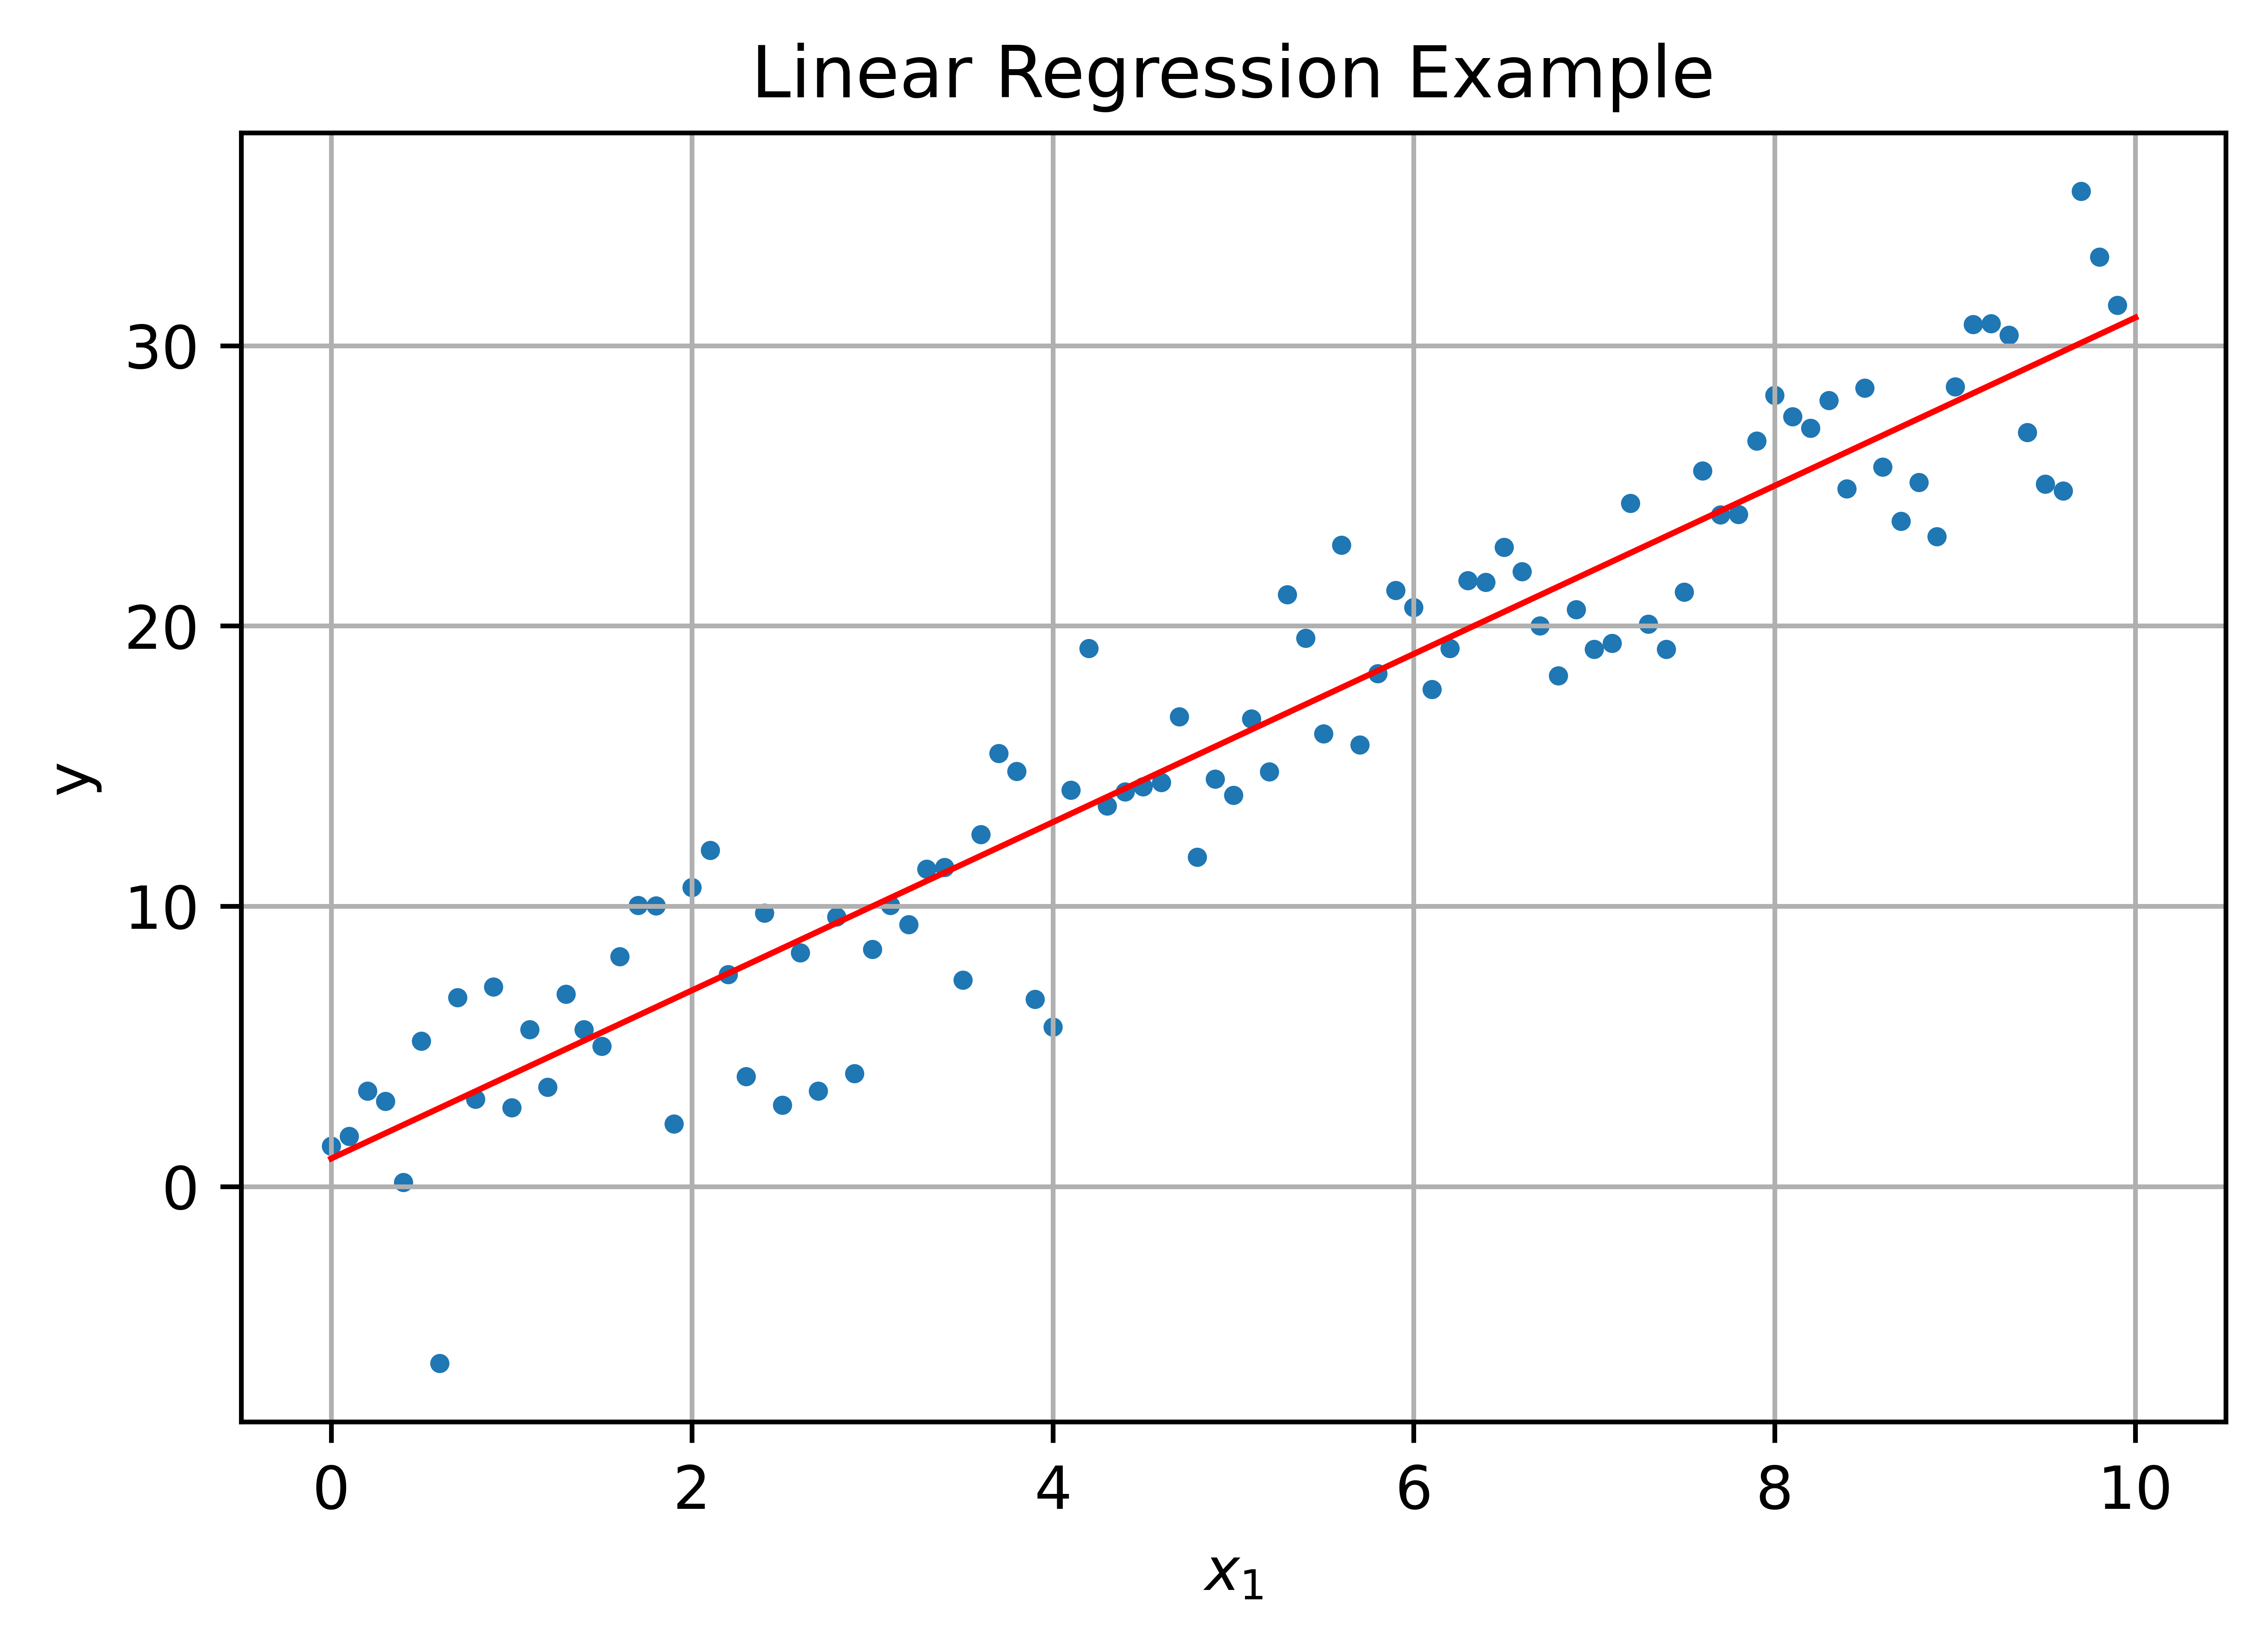
\includegraphics[width=70mm,scale=0.5]{images/regression_images/Regression_Example_Good_Fit.png}
        
            \caption*{This line is much better fitted to the data: $(\theta_0=1, \theta_1=3)$}
        \end{figure}
        
        What does this look like if we have \purp{two variables}? You need a 3D space, with 2 dimensions for the input.

        \begin{itemize}
            \item Each piece of data is a \purp{point} $(x_1,x_2, y)$.
            \item Our hypothesis is a \gren{plane}: for each pair $(x_1,x_2)$, it predicts a different $y$.
        \end{itemize}
        
        \begin{figure}[H]
        \centering
            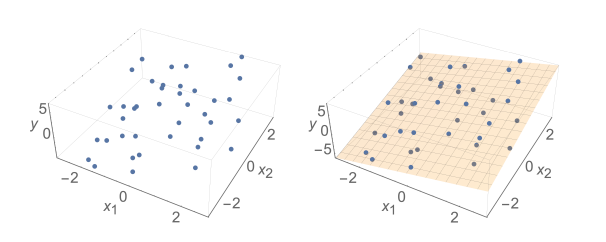
\includegraphics[width=100mm,scale=0.5]{images/regression_images/Regression_Plane.png}
        
            \caption*{This plane is \textbf{fitted} the same way our line was. Notice that $y$ is our \textbf{height}: this is the \textbf{output} of our regression.}
        \end{figure}
        
        Earlier, we mentioned that we can't really \purp{visualize} higher dimensions.
            \note{Looking at a 4D "plane" would be a headache.}
        
        \begin{itemize}
            \item So, instead, we don't even try to. We'll think of them in terms of our math. When we need intuition, we'll rely on the 2D plane.
            \item Because they're a higher-dimensional version of a \textbf{plane}, we call it a \vocab{hyperplane}.\\
        \end{itemize}
        
        \begin{definition}
            A \vocab{hyperplane} is a \purp{higher-dimensional version} of a \gren{plane} - a \gren{flat} surface that continues on forever.
            
            We use it to represent our \gren{linear} hypothesis for the purpose of \purp{regression}. 

            \begin{itemize}
                \item We have $d$ dimensions ($d$ variables) in our input.
                \item To represent our output, we need one additional, $\nth{(d+1)}$ dimension.
            \end{itemize}

            Visually, the "\purp{height}" of our plane represents the \orgg{output} of $h(x)$.
        \end{definition}

        \begin{itemize}
            \item Our line was a \textbf{1-D} object in a \textbf{2-D} plane.
            \item Our plane was a \textbf{2-D} object in a \textbf{3-D} space.
        \end{itemize}
        
        So, our \orgg{hyperplane} is a $d$ dimensional object in a $d+1$ dimensional space.

        \begin{itemize}
            \item Our goal is the same: we want our \vocab{hyperplane} to be as \textbf{close} to all of our data points as it possibly can.
        \end{itemize}

        
    \subsection{Another Interpretation}
    
        So far, we've generally interpreted our model similarly to $mx+b$.
        
        \begin{equation}
            h(x) = \red{\theta_0} + \red{\theta_1}x_1 + \red{\theta_2}x_2 + \red{\theta_3}x_3 + ... + \red{\theta_d}x_d
        \end{equation}

        \begin{itemize}
            \item Using our $\org{m}\grn{x}+b$ analogy, we can see $\org{\theta_k}$ as the "\orgg{slope}" of $\grn{x_k}$.

            \begin{equation}
                \pderiv{h}{x_k} = \theta_k
            \end{equation}
            
            \item In other words, $\theta_k$ tells us how much $x_k$ affects the \purp{output}.\\
        \end{itemize}

        \begin{concept}
            The \gren{larger} $||\theta_k||$ is, the \purp{more important} $x_k$ is to our output. 
            

            \begin{itemize}
                \item If we \gren{increase} $||\theta_k||$, then $x_k$ will have a \purp{bigger effect} on $h(x)$.
            \end{itemize}

            \begin{equation*}
                \overbrace{
                \pderiv{h}{x_k}
                }^{\text{Effect of $x_k$ on $h$}}= 
                \theta_k
            \end{equation*}

            This is a simple \orgg{pattern}: "as we change $x_k$, we change $h(x)$".
        \end{concept}

        We can also \gren{compare} each $\theta_k$ term to each other. 

        \begin{itemize}
            \item If $\theta_2$ is larger than $\theta_1$, then increasing $x_2$ would affect the output \orgg{more} than increasing $x_1$.

            \begin{equation}
                h(x) = 2x_1 + \overbrace{10000x_2}^{\text{$x_2$ has greater effect}}
            \end{equation}

            \item We could say that $x_2$ has a stronger effect on the output than $x_1$: it \gren{weighs more heavily} in the calculation.
        \end{itemize}
        
        
        Because of this, we sometimes call $\theta_k$ the \textbf{weight} for $x_k$.\\
        
        \begin{definition}
            A \vocab{weight} is a \orgg{parameter} that tells us how \gren{strongly} a variable influences our \purp{output}.
            
            It is usually a \purp{scalar} that we \gren{multiply} by our variable.
        \end{definition}

        \begin{itemize}
            \item We say that $\theta_0$ is an "offset", and the other $\theta_i$ terms are "weights".
        \end{itemize}

\pagebreak
%%%%%%%%%%%%%%%%%%%%%%%%%%%%%%%%%%%%%%%%%%%%%%%%%%%%%%%%%%%%%%%%%%%%%%%%%%%%%%%%%%%%%%%%%%%

\section{The stupidest possible linear regression algorithm}
    
    So, now we want to try to \purp{optimize} $J$ based on $\theta$ and $\theta_0$. How do we do that? Let's start as \gren{simple} as we possibly can.

    \phantom{}
    
    We can't try \textbf{every} possible $\Theta$, because there are an \purp{infinite} number of them. Rather than thinking too hard about a possible pattern, or an \textbf{algorithm}, let's just \orgg{randomly} try options.
    
    We'll try \textbf{random} values for $\theta$ and $\theta_0$, and \textbf{pick} whichever option gives us the \gren{best result}. Seems simple, if inefficient.

    \begin{figure}[H]
        \centering
            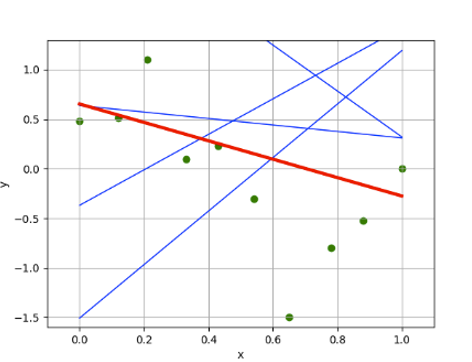
\includegraphics[width=70mm,scale=0.5]{images/regression_images/random_slopes.png}
        
            \caption*{Each line (hypothesis) was randomly generated. We focus on the red one: this is the best model, out of all the ones that we tried.}
        \end{figure}
    
    Why introduce such a silly algorithm? For a few reasons:
    
    \begin{itemize}
        \item It gives us an \textbf{example} of an optimization algorithm that's very \purp{simple}.
        \item \textbf{Randomly} generated results create a good \gren{baseline} - more intelligent algorithms can be compared to this one, to see how well we're doing.
            \note{Sometimes, you might come up with a clever technique, only to find out it isn't better than a random model! It happens more than you'd think.}
    \end{itemize}
    

\pagebreak
%%%%%%%%%%%%%%%%%%%%%%%%%%%%%%%%%%%%%%%%%%%%%%%%%%%%%%%%%%%%%%%%%%%%%%%%%%%%%%%%%%%%%%%%%%%

\section{Analytical solution: ordinary least squares}

    We can do \gren{better} than randomly \textbf{generate} parameters, though. In fact, in this rare case, we can actually \purp{solve} for optimal parameters!

    \phantom{}
    
    \subsection{Trying to Simplify}
        
        Our solution will involve a lot of algebra. Because of that, it's worth it to \gren{simplify} our formula as much as possible beforehand.
            \note{By algebra, we just mean "shuffling around math symbols in an equation".}
        
        \begin{equation}
            J(\theta,\theta_0) = 
                        \frac{1}{n}  \sum_{i=1}^n 
                        \left( 
                                \red{ (\theta^T} \blu{\ex{x}{i}} \red{ + \theta_0) 
                            }
                            - 
                                \blu{\ex{y}{i}}
                        \right)^2 
        \end{equation}
        
        Most parts of this equation can't really be \textbf{simplified}: $y$ and $x$ are just variables, and we can't do anything with the \textbf{sum} without knowing our data points.

        \begin{itemize}
            \item But, there's one notable detail: we \purp{separated $\theta_0$} from our other $\theta_k$ terms. 
            \item If we can \orgg{include $\theta_0$} in the dot product, our math will be easier.
        \end{itemize}
        

    \phantom{}
        
    \subsection{Combining $\theta$ and $\theta_0$}
        
         Let's go back to our \textbf{original} equation for $ (\theta^T x  + \theta_0)  $, before we switched to \purp{vectors}.
            \note{We drop the $\ex{}{i}$ notation whenever it isn't necessary, to de-clutter the equations. 
            
            \phantom{}
            
            Let's just say we've picked one random data point.}
        
        \begin{equation}
            h(x) \quad=\quad 
             \theta_0  + \theta \cdot x
            \quad=\quad 
            \red{\theta_0} + \theta_1x_1 + \theta_2x_2 + \theta_3x_3 + ... + \theta_dx_d
        \end{equation}
        
            We simplified our notation with a \gren{dot product}: each $\theta_k$ term is \textbf{multiplied} by an $x_k$ term.

        \begin{itemize}
            \item This is, of course, \orgg{excluding $\theta_0$}.
            \item We would end up with a simpler result if we could include $\theta_0$ in the $\theta$ vector. But, $\theta_0$ would need to be \purp{multiplied by an $x_0$ term}.
        \end{itemize}

        \begin{equation}
            h(x) = 
            \begin{bmatrix}
                \red{\theta_0} \\ \theta_1 \\ \vdots \\ \theta_d 
            \end{bmatrix}
            \cdot
            \overbrace{
            \begin{bmatrix}
                \blu{x_0} \\ x_1 \\ \vdots \\ x_d
            \end{bmatrix}
            }^{\text{We need $x_0$}}
        \end{equation}
        
        We have a trick: let's factor out \orgg{$x_0=1$}.
                    \note{You can always factor out 1 without changing the value!}
        
        
        \begin{equation}
            h(x) = \red{\theta_0}\blu{x_0} + \theta_1x_1 + \theta_2x_2 + \theta_3x_3 + ... + \theta_dx_d
        \end{equation}
        
        So, this means we just have to \textbf{append} a 1 to our vector $x$. At the \textbf{same time}, we'll append $\theta_0$ to $\theta$!
        
        \begin{equation}
            x = 
            \begin{bmatrix}
              \blu{1} \\ x_1 \\ x_2  \\ \vdots \\ x_d
            \end{bmatrix},
            \;\;\;\;\;\;\;\;\;\;\;\;\;\;\;
            \theta = 
            \begin{bmatrix}
              \red{\theta_0} \\ \theta_1 \\ \theta_2  \\ \vdots \\ \theta_d
            \end{bmatrix},
            \;\;\;\;\;\;\;\;\;\;\;\;\;\;\;
            h(x) = 
            \begin{bmatrix}
              \red{\theta_0} \\ \theta_1 \\ \theta_2  \\ \vdots \\ \theta_d
            \end{bmatrix}
            \cdot
            \begin{bmatrix}
              \blu{1} \\ x_1 \\ x_2 \\ \vdots \\ x_d
            \end{bmatrix}
        \end{equation}

        We'll write that symbolically, and then apply a transpose.
        
        \begin{equation}
            h(x) = \red{\theta} \cdot x = \blu{ \theta^T x }
        \end{equation}
        
        \begin{concept}
            Sometimes, to simplify our algebra, we can \orgg{append $\theta_0$} to $\theta$. 
            
            To make this possible, we \purp{choose $x_0=1$}.
            
            \begin{itemize}
                \item This requires \orgg{appending} a value of 1 to $x$.
            \end{itemize}
            
            Once we do this, we can \gren{write} 
            
            \begin{equation*}
                h(x)=\theta^T x
            \end{equation*}
        \end{concept}
        
        We \textbf{have} to append this 1 to every single $\ex{x}{i}$ in order for this to \textbf{work}. But, now we can treat our \gren{parameters} as \purp{one vector}.



    \pagebreak
    
    \subsection{Combining data points}

        There's another place we can clean things up:

        \begin{itemize}
            \item Currently, when using our \purp{objective} function, we have to \gren{sum} over \textbf{every} single data point.
                \note{Note that, for convenience, we've included $\theta_0$ in $\theta$.}
        \end{itemize}
    
        \begin{equation}
            J(\theta) = 
            \frac{1}{n}  \sum_{i=1}^n 
            \Big( \red{\theta^T} \blu{\ex{x}{i}}  - \blu{\ex{y}{i}}   \Big)^2
        \end{equation}

        \begin{itemize}
            \item This is a bit of a hassle - we have to consider every ($\ex{x}{i}, \ex{y}{i})$ term separately.

            \item Is there a better way?
        \end{itemize}
        
        We've solved this kind of problem before: using vectors above, we were able to work with \gren{many parameters} $\theta_k$ and \gren{many variables} $x_k$ at the same time.

            \begin{equation*}
            h(x) = \red{\theta_0} + \red{\theta_1}x_1 + \red{\theta_2}x_2 + \red{\theta_3}x_3 + ... + \red{\theta_d}x_d
            \xlongrightarrow{\text{vector form}} \quad
            h(x) = \theta^Tx
        \end{equation*}
        
        \begin{itemize}
            \item This made it easier to do lots of math quickly.\\
        \end{itemize}

        \begin{concept}
            One of the biggest benefits of \purp{matrices} is being able to do \gren{lots of math at the same time}.

            \begin{itemize}
                \item In particular, \vocab{matrix multiplication} allows you to do \gren{addition} and \purp{multiplication} on as many elements as you want.
            \end{itemize}
        \end{concept}
        
        Can we do the \textbf{same} here - combining \orgg{many data points} into one object?

    \phantom{}

    \subsection{Many data points in a matrix}

        We want to combine all of our data points into a single matrix. 

        \begin{itemize}
            \item We're already using \purp{rows} to represent \purp{multiple dimensions} of a data point. 
                \note{A reminder: a "dimension"(feature) is one aspect of our input data. For an animal, it might be height, weight, age, etc.
                
                \phantom{}
                
                Each dimension stores one piece of information.}

            \begin{equation}
                x = 
                    \begin{drcases}
                        \begin{bmatrix}
                            x_1 \\ x_2 \\ \vdots \\ x_d
                        \end{bmatrix}
                    \end{drcases}
                \text{ \lblu{ $\nth{k}$ dimension in row $k$} }
            \end{equation}

            \item We'll need different notation to separate \gren{data points}: we'll use \gren{columns}.
        \end{itemize}
    
        \begin{equation}
            X_{1D} =
                \overbrace{
                \begin{bmatrix}
                  \ex{x}{1} & \ex{x}{2} & \ex{x}{3} & \cdots & \ex{x}{n}
                \end{bmatrix}
                }^{\text{ \lblu{$\nth{i}$ data point in column $i$} }}
        \end{equation}
    
        \begin{definition}
            We use \purp{rows} to indicate the different \purp{dimensions} $x_k$ of a single data point, and \gren{columns} to indicate each \gren{data point} $\ex{x}{i}$.
    
            \begin{equation*}
                x = 
                    \begin{bmatrix}
                        \pur{x_1} \\ \pur{x_2} \\ \vdots \\ \pur{x_d}
                    \end{bmatrix}
                \qquad \qquad
                X_{1D} =
                    \begin{bmatrix}
                      \grn{\ex{x}{1}} & \grn{\ex{x}{2}} & \cdots & \grn{\ex{x}{n}}
                    \end{bmatrix}
            \end{equation*}
    
            \begin{itemize}
                \item Note that the capitalized $X$ matrix is used for \orgg{all of our data points $\ex{x}{i}$}.
            \end{itemize}
        \end{definition}

        \phantom{}

        These formats are both useful, but limited:

        \begin{itemize}
            \item $x$ can handle \purp{many dimensions}, but represents \gren{one data point}.
            \item $X_{1D}$ represents \gren{many data points}, but with only \purp{one dimension} for each.
        \end{itemize}

        Our solution? Combine them into a single object:\\

        \begin{kequation}
            $X$ is our \vocab{input matrix} in the shape \orgg{$(d \times n)$} contains information \gren{$n$ data points} with \purp{$d$ dimensions each}.
            
            \begin{equation*}
                X = 
                    \overbrace{
                        \begin{bmatrix}
                            \ex{x_1}{1} & \cdots  & \ex{x_1}{n} \\
                            \vdots      & \ddots & \vdots      \\
                            \ex{x_d}{1} & \cdots  & \ex{x_d}{n}
                        \end{bmatrix}
                        }^{ n \text{ data points}}
                    \bigggrB{50pt} d \text{ dimensions}
            \end{equation*}

        \end{kequation}

        \miniex Consider 3 data points in 2 dimensions: $[1,2]^T$, $[9,5]^T$, $[10,11]^T$.

        \begin{equation}
            \begin{bmatrix}
                1 \\ 2
            \end{bmatrix}, \;
            \begin{bmatrix}
                9 \\ 5
            \end{bmatrix}, \; 
            \begin{bmatrix}
                10 \\ 1
            \end{bmatrix}
            \quad \longrightarrow \quad 
            X = 
            \begin{bmatrix}
                1 & 9 & 10 \\
                2 & 5 & 1
            \end{bmatrix}
        \end{equation}

        If we want to replace $\theta^Tx +\theta_0$ with $\theta^Tx$, we can include 1's at the top:
            \note{Or the bottom, if we want.}

        \begin{equation}
            X = 
                \overbrace{
                    \begin{bmatrix}
                        1           & \cdots & 1           \\
                        \ex{x_1}{1} & \cdots  & \ex{x_1}{n} \\
                        \vdots      & \ddots & \vdots      \\
                        \ex{x_d}{1} & \cdots  & \ex{x_d}{n}
                    \end{bmatrix}
                    }^{ n \text{ data points}}
                \bigggrB{70pt} d+1 \text{ dimensions}
        \end{equation}
        
        We can do the same for $Y$: combine all of the data points into one matrix.\\
        
        \begin{kequation}
            $Y$ is our \vocab{output matrix} in the shape \purp{$(1 \times n)$} that contains all data points.
            
            \begin{equation*}
                Y = 
                    \begin{bmatrix}
                        \ex{y}{1} & \cdots & \ex{y}{n}
                    \end{bmatrix}
            \end{equation*}
        \end{kequation}

            \note{Why is this a row vector, not a matrix? 
            
            \phantom{}

            This is a \purp{regression} problem: each output is a scalar, not a vector!}

    \pagebreak

    \subsection{Objective Function in matrix form}

        Now that we can use all of our \gren{data points} at the same time, we can condense our objective function.

        \begin{equation}
            J(\Theta) = 
            \frac{1}{n}  \sum_{i=1}^n 
            \Big( \red{\theta^T} \blu{\ex{x}{i}}  - \blu{\ex{y}{i}}   \Big)^2
        \end{equation}

        We can simultaneously compute $(\red{\theta^T} \blu{\ex{x}{i}}  - \blu{\ex{y}{i}})$ for all of our data points at the same time:
            \note{We could show that this matrix multiplication gives the results we want, with calculation.
            
            \phantom{}
            
            But this is a little tedious, and doesn't teach us much, so we recommend trying it yourself if you're unconvinced.}

        \begin{equation*}
            \red{\theta^T} \blu{X} - \blu{Y}  \qquad=\qquad 
            \begin{bmatrix}
                \theta^T \ex{x}{\grn{1}}  - \ex{y}{\grn{1}} &&&
                \theta^T \ex{x}{\red{2}}  - \ex{y}{\red{2}} &&&
                \cdots &&&
                \theta^T \ex{x}{\org{n}}  -  \ex{y}{\org{n}}
            \end{bmatrix}
        \end{equation*}

        This isn't exactly what we want, though: we want $(\red{\theta^T} \blu{\ex{x}{i}}  - \blu{\ex{y}{i}})^2$: multiplied by itself. We can do this with a \gren{dot product}:

        \begin{equation}
            \Big( \red{\theta^T} \blu{\ex{x}{i}}  - \blu{\ex{y}{i}} \Big)^2 
            \quad \longrightarrow \quad
            \Big( \red{\theta^T} \blu{X} - \blu{Y} \Big) \cdot 
            \Big( \red{\theta^T} \blu{X} - \blu{Y} \Big)
        \end{equation}

        How do we write this dot product with matrix multiplication?\\

        \begin{clarification}
            When $a$ and $b$ were \purp{column vectors}, we could take their dot product as $a^Tb$.

            \begin{equation*}
                a = 
                \begin{bmatrix}
                    a_1 \\ a_2 \\ \vdots \\ a_m
                \end{bmatrix}
                \quad 
                b = 
                \begin{bmatrix}
                    b_1 \\ b_2 \\ \vdots \\ b_m
                \end{bmatrix}
                \quad \implies \quad
                a \cdot b = a^Tb
            \end{equation*}

            But we have to do the opposite for \gren{row vectors} $p$ and $q$: we get $pq^T$.

            \begin{equation*}
                \begin{matrix}
                    p = 
                \begin{bmatrix}
                    p_1 & p_2 & \cdots & p_m
                \end{bmatrix} \\\\
                q = 
                \begin{bmatrix}
                    q_1 & q_2 & \cdots & q_m
                \end{bmatrix}
                \end{matrix}
                \quad \implies \quad
                p \cdot q = pq^T
            \end{equation*}
        \end{clarification}

            \note{Here, we're comparing $a^Tb$ to $ab^T$.}

        Because $(\red{\theta^T} \blu{X} - \blu{Y}) $ is a \purp{row vector}, we'll have to write it in the $pq^T$ format:

        \begin{equation}
            \Big( \red{\theta^T} \blu{\ex{x}{i}}  - \blu{\ex{y}{i}} \Big)^2 
            \quad \longrightarrow \quad
            \Big( \pur{\theta^T X - Y} \Big) 
            \Big( \pur{\theta^T X - Y} \Big)^T
        \end{equation}

        This formula represents our original objective function:

        \begin{equation}
            \frac{1}{n}\Big( \pur{\theta^T X - Y} \Big) 
            \Big( \pur{\theta^T X - Y} \Big)^T
            \quad=\quad
            \frac{1}{n}  \sum_{i=1}^n 
            \Big( \red{\theta^T} \blu{\ex{x}{i}}  - \blu{\ex{y}{i}}   \Big)^2
        \end{equation}

        

        \begin{kequation}
            Using $X$, $Y$, and $\theta$ can write our \gren{objective function} for \purp{multiple} variables and \purp{multiple} data points as
            
            \begin{equation*}
                J(\theta) = \frac{1}{n}
                    \Big( \red{ \theta^T X - Y} \Big)
                    \Big( \red{ \theta^T X - Y} \Big)^T
            \end{equation*}
        \end{kequation}

            \note{Because $n$ is a constant, we sometimes ignore it when we're minimizing $J(\Theta)$.}

        \phantom{}

        
        It is important to \textbf{remember} the \textbf{shape} of our objects, as well.\\
        
        \begin{concept}
            Our matrices have the shapes:
            
            \begin{itemize}
                \item $X$:        $(d \times n)$ - matrix
                \item $Y$:        $(1 \times n)$ - row vector\\
                
                \item $\theta$:   $(d \times 1)$ - column vector
                \item $\theta_0$: $(1 \times 1)$ - scalar\\
                
                \item $J$:        $(1 \times 1)$ - scalar
            \end{itemize}
            
            If we combine $\theta_0$ into $\theta$, replace every use of \red{$d$} with \blu{$d+1$}.
            
        \end{concept}
        
        \note{Notice that these shapes make sense for our above equation! Try working through the matrix multiplication to verify this.}
        
        These shapes are worth \textbf{memorizing}.

        \phantom{}
        
    \subsection{Alterate Notation}
    
        One side problem: some ML texts use the \textbf{transpose} of $X$ and $Y$.\\
    
        \begin{notation}
            Some subjects use \vocab{different notation} for \vocab{matrices}. The main difference is that $X$ and $Y$ use their \purp{transpose}, which we'll notate as
        
            \begin{equation*}
                \Xt = X^T \;\;\;\;\;\;\;\; \Yt = Y^T
            \end{equation*}
            
            Thus, our equation above becomes
            
            \begin{equation*}
                J = \frac{1}{n}
                    \Big( \red{ \Xt \theta  - \Yt } \Big)^T
                    \Big( \red{ \Xt \theta  - \Yt } \Big) 
            \end{equation*}
        \end{notation}

    \pagebreak
        
    \subsection{Optimization in 1-D - Using Calculus}

        Now that we've sorted our data, we can start \purp{optimizing} $\theta$. Our goal is to modify $\theta$, to find the minimal $J$.
            \note{We're gonna focus on one data point/dimension at a time, so we don't need our matrix notation.}

        \begin{equation}
                J(\theta) = 
                \frac{1}{n}  \sum_{i=1}^n 
                \left( \red{\theta^T} \blu{\ex{x}{i}}  
                - \blu{\ex{y}{i}} \right)^2 
            \end{equation}
        
        We'll start with a simplified case, and build our way up:

        \begin{itemize}
            \item First, we limit our attention to one data point ($n=1$):

                \begin{equation}
                    J(\theta) =(\red{ \theta^T} \blu{x}   - \blu{y} )^2
                \end{equation}

            \item And we'll assume $\theta$ and $x$ are one-dimensional ($d=1$).

                \begin{equation}
                    J(\theta) = (\red{\theta} \blu{x}   - \blu{y} )^2
                \end{equation}
        \end{itemize}

        \phantom{}
        
        
        If we use $\theta$ as a \textbf{variable}, this is an ordinary single-variable function! How would we find the \purp{minimum}? 

        \begin{itemize}
            \item Using \textbf{calculus}! Anywhere there's a local \textbf{minimum}, we typically know the \gren{derivative is 0}.
                \note{Assuming a "smooth" surface...}\\
        \end{itemize}

        \begin{concept}
            
            If our function $J(\theta)$ has \gren{one variable}, we find possible \vocab{local minima} $\theta$ wherever the \purp{derivative} $\pderivslash{J}{\theta}$ is zero.
            
            \begin{equation*}
                \pderiv{J}{\theta}=0
            \end{equation*}

            \phantom{}

            \begin{itemize}
                \item To make sure it's a minimum (not a maximum), we also need to make sure that the \orgg{second derivative} is positive ($J''(\theta)>0)$.

                \item We already know this is true for \purp{squared loss}, so we won't bother with this step.
            \end{itemize}
        \end{concept}

            \note{Why do we need $\pderivslash{J}{\theta}=0$? 
            
            \phantom{}
            
            If $\pderivslash{J}{\theta}>0$, then decreasing $\theta$ slightly would reduce $J$: there's a lower point nearby, so this isn't a minimum!
            
            \phantom{}
            
            If $\pderivslash{J}{\theta}<0$, increasing $\theta$ has the same effect.}

        \begin{itemize}
            \item Note that we're taking $\pderiv{}{\theta}$, \redd{not} $\pderiv{}{x}$.
            \item This is because our goal is to modify $\theta$ (our model), not $x$ (our data).
                \note{We want to train our model to match our data, not the other way around!}
        \end{itemize}

        Let's do this for our simple example:
        
        \begin{equation}
            J'(\theta) = 2\blu{x}(\red{\theta} \blu{x} - \blu{y} ) = 0
        \end{equation}
        
        We just find where the slope $J'(\theta)$ is 0, and solve for $\theta$!
            \note{Because this is the optimal $\theta$, we call it $\theta^*$.}
        
        \begin{equation}
            \theta^* = \frac{y}{x}
        \end{equation}

        

    \phantom{}
        
    \subsection{Optimizing for multiple variables}

        This time, we'll do \gren{one data point}, having \purp{$d$ dimensions}.

        \begin{itemize}
            \item This gets a bit tricky, because we have to do our math with \orgg{vectors}.
                \note{Because we only have one data point, we'll omit the $\ex{}{i}$ notation.}
        \end{itemize}
        
        \begin{equation}
            J(\theta) = (\red{ \theta^T x  } - y )^2
        \end{equation}
        
        We'll \textbf{optimize} this. In the \gren{one-dimensional} case, we wanted to set the \textbf{derivative} of $J$ to \purp{zero}, using a single $\theta$ variable.
        
        \begin{itemize}
            \item Now, we have \orgg{multiple variables} $\theta_k$ that we could optimize.

            \item How do we know when we've optimized all of them?
        \end{itemize} 

        Well, if we consider each dimension separately, $\theta_k$ would be optimized if 

        \begin{equation}
            \pderiv{J}{\theta_k} = 0
        \end{equation}
        
        
        So, maybe it would be reasonable to just set \purp{every} derivative to \textbf{zero}? 
        
        \begin{itemize}
            \item It turns out, the answer is \textbf{yes}! 
                \note{We can use the reasoning that we used for 1D:
                
                \phantom{}
                
                If one of our derivatives $\pderivslash{J}{\theta_k} > 0$, then we could decrease $\theta_k$ to find a nearby point which is "lower" than our current point: we don't have a minimum.
                
                \phantom{}
                
                Thus, every derivative must be 0.}
        \end{itemize}
        
        
        If every individual derivative $\pderivslash{J}{\theta_k}$ is zero, we have a potential minimum.\\
        
        \begin{concept}
            If our function $J(\theta)$ has \red{$d+1$} \gren{parameters}, we find possible \vocab{local minimum} $\theta$ anywhere that obeys the system of equations
            
            \begin{equation*}
                \begin{matrix}
                    \pderiv{J}{\theta_{\red{0}}} = 0 &&
                \pderiv{J}{\theta_{\red{1}}} = 0 &&
                \pderiv{J}{\theta_{\red{2}}} = 0 &&
                \dots &&
                \pderiv{J}{\theta_{\red{d}}} = 0
                \end{matrix}
            \end{equation*}
            
            Or in general, 
            
            \begin{equation*}
                \pderiv{J}{\theta_{\red{k}}} = 0 \qquad \qquad \text{ for all $k$ in $\setty{0, 1, 2, \dots, d }$}
            \end{equation*}

            \begin{itemize}
                \item Why $d+1$ parameters instead of $d$? Because we're including $\theta_0$ as one additional parameter.
            \end{itemize}
            
        \end{concept}
        
        \note{Again, we ignore the second requirement of making sure this isn't a \textbf{maximum} or \textbf{saddle} point.}
        
        The \purp{solution} to this system of equations will be our \textbf{desired list of parameters}, $\theta^*$.

        \begin{equation}
            \theta^* = 
            \begin{bmatrix}
                \theta^*_1 \\ \theta^*_2 \\ \vdots \\ \theta^*_d
            \end{bmatrix}
        \end{equation}

    \phantom{}
        
    \subsection{Gradient Notation}

        Above, we wrote our derivative \purp{element-wise}: each derivative got its own equation.

        \begin{itemize}
            \item We can make things easier by storing our derivatives in a \orgg{column vector}, just like how $\theta$ stores $\theta_k$ terms.
                \note{How do we know that this is a column vector, and not a row vector? 
                
                \phantom{}
                
                Check out the matrix derivative notes for a complete explanation.}
        \end{itemize}

        \begin{equation}
            \pderiv{J}{\theta} = 
            \begin{bmatrix}
                \pderivslash{J}{\theta_0}\\
                \pderivslash{J}{\theta_1}\\
                \vdots \\
                \pderivslash{J}{\theta_d}\\
            \end{bmatrix}
        \end{equation}

        We'll think of this as a bigger, \gren{multivariable} derivative, called the \vocab{gradient}.
            \note{We'll give more conceptual intuition for the gradient in the next chapter. Look forward to it!}\\
        
        \begin{kequation}
            The \vocab{gradient} of $J$ with respect to $\theta$ is
            
            \begin{equation*}
                \nabla_\theta J 
                \quad=\quad
                \pderiv{J}{\theta} 
                \quad=\quad
                \begin{bmatrix}
                    \pderivslash{J}{\theta_0} \\
                    \pderivslash{J}{\theta_1} \\
                    \vdots \\
                    \pderivslash{J}{\theta_d}
                \end{bmatrix}
            \end{equation*}

            It has the same dimensions $(d \times 1)$ as $\theta$.
        \end{kequation}

            \note{Why is $\pderivslash{J}{\theta}$ a $(d \times 1)$ matrix instead of $(1 \times d)$? 
            
            \phantom{}
            
            We don't have a special reason: it's a convention we've picked, that works well with the rest of our math.
            
            \phantom{}
            
            In fact, some other texts might do differently. To learn more about our rules, check the Matrix Derivatives notes.}
        
        Now, we can rewrite our previous rule, "every derivative is 0":
        
        \begin{equation}
            \nabla_\theta J =
            \begin{bmatrix}
                \pderivslash{J}{\theta_0} \\
                \vdots \\
                \pderivslash{J}{\theta_d}
            \end{bmatrix}
            = 
            \begin{bmatrix}
                0 \\
                \vdots \\
                0
            \end{bmatrix}
            =
            \vec{0}
        \end{equation}
        
        
        \begin{concept}
            If $\theta$ is a \purp{vector}, we can find possible \vocab{local minima} $\theta$ of $J(\theta)$ anywhere that the \gren{gradient} $\nabla_{\theta}J$ is zero. 
            
            \begin{equation*}
                \nabla_\theta J=\vec{0}
            \end{equation*}

        \end{concept}
        
        \note{Once again: we should check if it's a minimum. But we continue to ignore this caveat.}
        
        This is the general equation we \orgg{solve} to find $\theta^*$.



    \phantom{}
        
    \subsection{Matrix Calculus}

        Now, we return to the general case: \gren{$n$ data points}, each having \purp{$d$ dimensions}.

        \begin{equation*}
            J(\theta) = \frac{1}{n}
                \Big( \red{ \theta^T X - Y} \Big)
                \Big( \red{ \theta^T X - Y} \Big)^T
        \end{equation*}

        Using the "alternate" notation":
        
        \begin{equation}
            J = \frac{1}{n}
                \left( \blu{ \Xt \theta  - \Yt } \right)^T
                \left( \blu{ \Xt \theta  - \Yt } \right) 
        \end{equation}
        
        We will \purp{not} show how to take this matrix derivative. But our result is:
            \note{Want to know how? Check out A.4 in the official appendix.}

        \begin{equation}
            \nabla_\theta J = 
                \frac{2}{n} \Xt^T
                \left( \blu{ \Xt \theta  - \Yt } \right) 
            =0
        \end{equation}

        \begin{clarification}
            Note that matrix derivatives often look \gren{similar} to traditional, single-variable derivatives. However, they are \redd{not the same}.

            \begin{itemize}
                \item Often, this can result in \purp{shape errors}: we end up with the wrong matrix shape.
            \end{itemize}
        \end{clarification}

            \note{How do we take a matrix derivative in general? Check out an explanation in the Matrix Derivatives chapter.}
        
        
        From here, we just solve for $\theta$, using matrix multiplication rules.\\
        
        \begin{kequation}
        
            The \vocab{solution} for \vocab{OLS optimization} is 
            
            \begin{equation*}
                \theta = 
                \underbrace{ 
                \inv{ \left(  \Xt^T\Xt  \right)  }
                }_{d \times d}
                \underbrace{
                \Xt^T
                }_{d \times n}
                \underbrace{
                \Yt
                }_{n \times 1} 
            \end{equation*}
            
            Or, in our \purp{original} notation,
            
            \begin{equation*}
                \theta = 
                \underbrace{ 
                \inv{ \left(  XX^T  \right)  }
                }_{d \times d}
                \underbrace{
                X
                }_{d \times n}
                \underbrace{
                Y^T
                }_{n \times 1} 
            \end{equation*}

            \phantom{}

            \begin{itemize}
                \item If $\theta_0$ is included in $\theta$, then dimension $d$ is replaced with $d + 1$.
            \end{itemize}
            
        \end{kequation}

            \note{Note that this requires that $XX^T$ is invertible: we need to compute that inverse $(XX^T)^{-1}$ in the equation, after all.
            
            \phantom{}
            
            This technique doesn't work if that's not the case. But, we'll introduce a different technique to solve this problem: regularization!}

        
        
    We've finished with "ordinary least squares".
    
    \begin{itemize}
        \item We call it "ordinary" because this is the \gren{simple} version of the problem.
        \item We'll make it more complex by introducing \orgg{regularization}.
    \end{itemize}

        
\pagebreak
%%%%%%%%%%%%%%%%%%%%%%%%%%%%%%%%%%%%%%%%%%%%%%%%%%%%%%%%%%%%%%%%%%%%%%%%%%%%%%%%%%%%%%%%%%%

\section{Regularization}

    The above solution gives us the \gren{best} model for matching our \purp{training data}.

    \begin{itemize}
        \item But earlier, we mentioned that we want our model to be able to \orgg{generalize} to new data.
            \note{Because our training data doesn't perfectly reflect all of our future data.}
    \end{itemize}

    We need some math to represent this goal of "generality".

    \begin{itemize}
        \item This equation won't measure our performance on training data, but instead encourages us to do well on \purp{future data}.
    \end{itemize}
        
    We call this type of function a \vocab{regularizer}.\\
    
    \begin{definition}
        A \vocab{regularizer} is a term to our \gren{objective function} that helps measure how \purp{general} our hypothesis is.

        \begin{itemize}
            \item By \gren{optimizing} this term, we hope to create a model that works better with \purp{new data} we didn't train with.
        \end{itemize}
        
        This function takes in our \purp{vector of parameters} \gren{$\Theta$} as an input: \purp{$R(\Theta)$}.
    \end{definition}

    But how do we make a model "more general?"

    \begin{itemize}
        \item First, we need to \gren{understand} the problem: \purp{what's wrong} with only using our training data?
        
    \end{itemize}


    

    \phantom{}

    \subsection{Coincidences, and fake patterns}

        The goal of our model $\theta$ is to look for \purp{patterns}. This is a concept we discussed earlier (section 2.3.8):\\

        \begin{concept}
            \textit{(Review)}
            
            The \gren{larger} $||\theta_k||$ is, the \purp{more important} $x_k$ is to our output. 
            

            \begin{itemize}
                \item If we \gren{increase} $||\theta_k||$, then $x_k$ will have a \purp{bigger effect} on $h(x)$.
            \end{itemize}

            \begin{equation*}
                \overbrace{
                \pderiv{h}{x_k}
                }^{\text{Effect of $x_k$ on $h$}}= 
                \theta_k
            \end{equation*}

            This is a simple \gren{pattern}: "as we change $x_k$, we change $h(x)$ by this much".
        \end{concept}

        $\theta$ is trying to identify \orgg{which variables} have an effect on our output, and by how much.
            \note{$\theta_k<0$ doesn't mean that $x_k$ doesn't matter: it just means that it affects $h(x)$ by decreasing it, instead of increasing it.}

        \begin{itemize}
            \item If $||\theta_k||$ is large, our models thinks that $x_k$ is important to our output.
        \end{itemize}

        Our goal is to modify each $\theta_k$ term until it matches the real distribution.

        

        \phantom{}

        But seeing a pattern ($x_k$ affecting $h(x)$) doesn't mean that it's real: \purp{random chance} can cause us to see patterns that don't really exist.

        \begin{itemize}
            \item \miniex You take 20 quizzes during a semester. Every time you did \gren{well}, you happened to be wearing a \redd{red shirt}.
            
            \item You might come to believe that red shirts help you study \gren{better}, even though it was just luck.
        \end{itemize}

        Isn't this kind of coincidence a bit unlikely? Maybe. 

        \begin{itemize}
            \item But what happens if we have 10 possible coincidences? It's less likely that we avoid all of them.
                \note{Suppose the chance of one coincidence is $p$.
                
                \phantom{}
                
                The chance of \gren{one} coincidence not occurring is $(1-p)$. The chance of \purp{ten} coincidences not occurring is $(1-p)^{10}$.

                \phantom{}
                
                As we get more chances, we're more likely to see a coincidence.}

            \item In other words: the more \orgg{opportunities} there are for something rare to happen, the \gren{more likely} it is to happen.\\
        \end{itemize}


        \begin{concept}
            The more \gren{patterns} we're looking for, the more likely that \textbf{at least one} of the them shows up by \orgg{coincidence}.

            \begin{itemize}
                \item Our data can, by chance, match a pattern that \purp{isn't even real}. 
            \end{itemize}
        \end{concept}
        
            \note{For some entertaining examples, search the phrase "spurious correlation".}

        This really becomes a problem for our model: often, we \purp{don't know} what data matters, so we include \gren{everything} we possibly can.

        \begin{itemize}
            \item But the more data we include, the more likely that something looks \gren{important} on \orgg{accident}!
        \end{itemize}

        This is an interesting situation, where \gren{learning more} about our training data can cause our model to perform \purp{worse}: we're \vocab{overfitting}.
            \note{Learning more about our training data isn't necessarily the same as learning more about the true distribution that data came from!}\\

        \begin{definition}
            \textit{(Review from Introduction chapter)}

            \vocab{Overfitting} occurs whenever we \gren{learn} ("fit") our training data too exactly, and it causes problems when we see \purp{new data}.

            \begin{itemize}
                \item Often, we \orgg{memorize} very specific patterns, that don't actually hold up in general: they only appeared in our randomly sampled training data. 
            \end{itemize}
        \end{definition}

        \miniex You flip a coin 10 times, and it comes up heads 8 times.

        \begin{itemize}
            \item You've decided that the coin has an 80\% chance of coming up heads.

            \item But it's a fair coin: the 'training data' (10 coin flips) doesn't match the 'true distribution' (50\% chance of heads).
        \end{itemize}

        Now, we understand our problem. Let's come up with a solution.


    \phantom{}

    \subsection{Ridge Regression}

        We're worried about our model \purp{finding false patterns} based on weak evidence.

        \begin{itemize}
            \item If our model finds a \gren{pattern}, then it'll increase $||\theta_k||$: it considers $x_k$ to be important for predicting $h(x)$, because the data coincidentally makes it \purp{look} important.
        \end{itemize}

        If our model is "too eager" to find patterns, we can make it \orgg{more skeptical} of patterns it might see.
            \note{It still need to look for \textit{some} (hopefully real) patterns, so that it can make good predictions $h(x)$.}

        \begin{itemize}
            \item In other words, we'll \purp{punish} our model for increasing $||\theta_k||$ too easily.
                \note{We'll actually use $\theta_k^2$, for the same reasons we use squared loss: 
                
                \phantom{}
                
                Smoother, works well for positive and negative $\theta_k$, etc.}\\
        \end{itemize}

        \begin{concept}
            We want to \purp{discourage} our model from prematurely deciding that $x_k$ has a \orgg{effect} on $h(x)$.

            \begin{itemize}
                \item Thus, we'll \gren{discourage} our model from increasing $||\theta_k||$: $\pur{\theta_k}$ represents this "\orgg{effect}".
            \end{itemize}

            \begin{equation*}
                R(\theta_k) = \theta_k^2
            \end{equation*}

            \begin{itemize}
                \item Our algorithm will \purp{minimize} $R(\Theta)$, so we'll make this $\theta_k^2$ \gren{small}.
            \end{itemize}
        \end{concept}

        We can repeat this process for all of our $\theta_k$ terms, and combine them into a vector $\theta$:

        \begin{equation*}
            R(\Theta) = \sum_k \pur{\theta_k^2} 
            \quad=\quad \abs{|\theta|}^2 = \theta \cdot \theta
        \end{equation*}

        This is our \orgg{ridge regression} model.
            \note{Why "ridge regression"? We'll get into that later.}\\

        \begin{kequation}
            Our \redd{regularizer for regression} will be given by \purp{square magnitude} of $\theta$:
            
            \begin{equation*}
                R(\Theta) = \norm{\theta}^2 = \theta^T\theta
            \end{equation*}

            \begin{itemize}
                \item In this model, we are biasing $\norm{\theta}$ towards 0: the farther from 0 we are, the more we punish the model.
            \end{itemize}
            
            This approach is called \vocab{Ridge Regression}.
        \end{kequation}

    \phantom{}

    \subsection{$\lambda$, our regularization constant}

        We can now create an "\purp{objective function}" that includes training loss, \textbf{and} regression.

        \begin{equation}
            J(\theta) = 
                        \frac{1}{n}  \sum_{i=1}^n 
                        \left( 
                            \underbrace{
                                \red{(\theta^T \ex{x}{i}  
                                + \theta_0)}
                            }_{guess}
                            - \underbrace{
                                \blu{\ex{y}{i}} 
                            }_{answer}
                        \right)^2 
                        + 
                        \underbrace{
                            \pur{ \norm{\theta}^2 }
                        }_{Regularizer}
        \end{equation}

        Notice that these terms "compete" with each other:\\

        \begin{concept}
            Our \gren{training loss} and \purp{regularizer} compete with one another, affecting our model in opposing ways:

            \begin{itemize}
                \item Our regularizer wants us keep $\theta$ small, being more \gren{suspicious} of predicting patterns.

                \item But in order to make good predictions for our \purp{training data}, we need to find the \orgg{real} patterns: some $\theta$ values need to be bigger, to predict our data.
            \end{itemize}
        \end{concept}

            \note{This is why we don't end up with model $\theta=\vec{0}$: while this model would have low \purp{regularization} $R(\Theta)$, it'll have high \gren{training loss}.}


        We need a \gren{balance} between training loss and regularization. It would be useful to have a way to \orgg{control} that balance.

        \begin{itemize}
            \item That way, we can decide, "how much do we care about matching training data, versus avoiding coincidental patterns?"
        \end{itemize}

        We have a tool for this: we'll represent "how much we care about \redd{regularization}" with a \vocab{constant} \red{$\lambda$}.\\

        \begin{definition}
            \vocab{Lambda}, or \vocab{$\lambda$}, is the constant ($\lambda \geq 0$) we \gren{scale} our \purp{regularizer} by.

            \begin{equation*}
                \text{Total Regularization} \quad=\quad  \lambda R(\Theta) 
                \quad = \quad \lambda ||\theta||^2
            \end{equation*}
            
            It represents \gren{how strongly} we want to regularize: the larger it is, the more strongly we try to \purp{generalize} our model.

        \end{definition}

        Why is $\lambda \geq 0$?\\

        \begin{clarification}
            We keep $\lambda \geq 0$, because $\lambda<0$ would encourage our model to make $||\theta||$ \gren{bigger}, no matter what.

            \begin{itemize}
                \item There's a limit to how small $|\theta|$ can be, but there's \purp{no limit} on how big it can be: it would just keep getting bigger forever.
            \end{itemize}
        \end{clarification}

        Finally, we have our \purp{completed} objective function:\\

        \begin{kequation}
            The \vocab{objective function} for \vocab{ridge regression} is given as 
            
            \begin{equation*}
                J(\Theta) = 
                            \frac{1}{n}  \sum_{i=1}^n 
                            \left( 
                                \underbrace{
                                    \red{(\theta^T \ex{x}{i}  
                                    + \theta_0)}
                                }_{guess}
                                - \underbrace{
                                    \blu{\ex{y}{i}} 
                                }_{answer}
                            \right)^2 
                            + 
                            \underbrace{
                                \pur{ \lambda \norm{\theta}^2 }
                            }_{Regularizer}
            \end{equation*}
        \end{kequation}

            \note{Readers might catch that our regularizer doesn't include $\theta_0$. There's a good reason for that! We'll discuss it below.}

        Once again, we note the contrast between "training loss" and "regularization".

        \begin{itemize}
            \item We've only made one change: $\lambda$ can increase or decrease our focus on regularization.
        \end{itemize}

        This $\lambda$ is crucial to our model: the larger it is, the more we punish our model for increasing $||\theta||$.\\

        \begin{concept}
            The more \vocab{regularization} (large $\lambda$) we have, the more we're \purp{focused} on keeping $|\theta|$ small.

            \begin{itemize}
                \item If we make $\lambda$ \gren{too big}, then $||\theta||$ becomes \purp{very small}: our model doesn't learn enough information.

                \item If we make $\lambda$ \gren{too small}, then $||\theta||$ becomes \purp{very big}: our model learns \orgg{all} the patterns of our data, even the ones that come from random noise.
            \end{itemize}
        \end{concept}




    \pagebreak

    \subsection{Why not regularize $\theta_0$?}

        Note that when we regularize with $\pur{ \lambda \norm{\theta}^2 }$, we're \orgg{not including $\theta_0$} in our vector:

        \begin{equation}
            R(\Theta) = \lambda \theta^T\theta \qquad \qquad 
            \theta = \begin{bmatrix}
                \red{\theta_1} \\ \theta_2 \\ \vdots \\ \theta_d
            \end{bmatrix}
        \end{equation}

        This suggest that we're \purp{not regularizing} $\theta_0$. Why is that?\\

        \begin{concept}
            We \orgg{do not regularize} $\theta_0$.

            \begin{itemize}
                \item We \gren{allow} $\theta_0$ to take whatever value fits best.
            \end{itemize}
        \end{concept}

        The first reason: $\theta_0$ works \purp{differently} from our other $\theta_k$ terms.

        \begin{itemize}
            \item A term $\theta_k$ tell us how \gren{important} one variable $x_k$ is to our output $h(x)$.

            \item $\theta_0$ works almost the opposite way: it \orgg{ignores} our input $x$, and gives a baseline output.

                \begin{itemize}
                    \item In other words: if we \purp{remove} the effect of all of our variables ($x=\vec{0}$), what do we expect to see?
                        \note{If our input data is centered on $x=\vec{0}$ (equally above and below on each axis), $\theta_0$ is the \gren{average} output we expect to see.}
                \end{itemize}
        \end{itemize}

        Naturally, regularization has very different effects:

        \begin{itemize}
            \item If you regularize $||\theta_k||$, your model i will emphasize the \orgg{effect} of $x_k$ by a smaller amount. 
            
            \item If you regularize $||\theta_0||$, you've just \gren{shifted} every output, by the same amount.\\
        \end{itemize}

        \begin{concept}
            Unlike $\theta_k$, $\theta_0$ doesn't find \orgg{patterns} in the data: it just tells us roughly how \purp{large} our output is.

            \begin{itemize}
                \item In fact, $||\theta_0||$ affects all of our data in the \gren{exact same way}.

                \item Decreasing $||\theta_0||$ would shift all outputs equally: this doesn't do anything to make it more \gren{accurate} for future data.
            \end{itemize}

            Because of this difference, it's not necessary to \orgg{regularize} $\theta_0$.
        \end{concept}

        \phantom{}

        Another reason we don't regularize $\theta_0$ is that it's often \orgg{necessary} for good predictions. This is best shown with a \textbf{visual} example.

        \begin{itemize}
            \item Let's take an example with one input, $x_1$. So, we have a \purp{linear} function: \red{$h(x) = \theta_1x_1+\theta_0$}.
        \end{itemize}
        
        \begin{figure}[H]
        \centering
            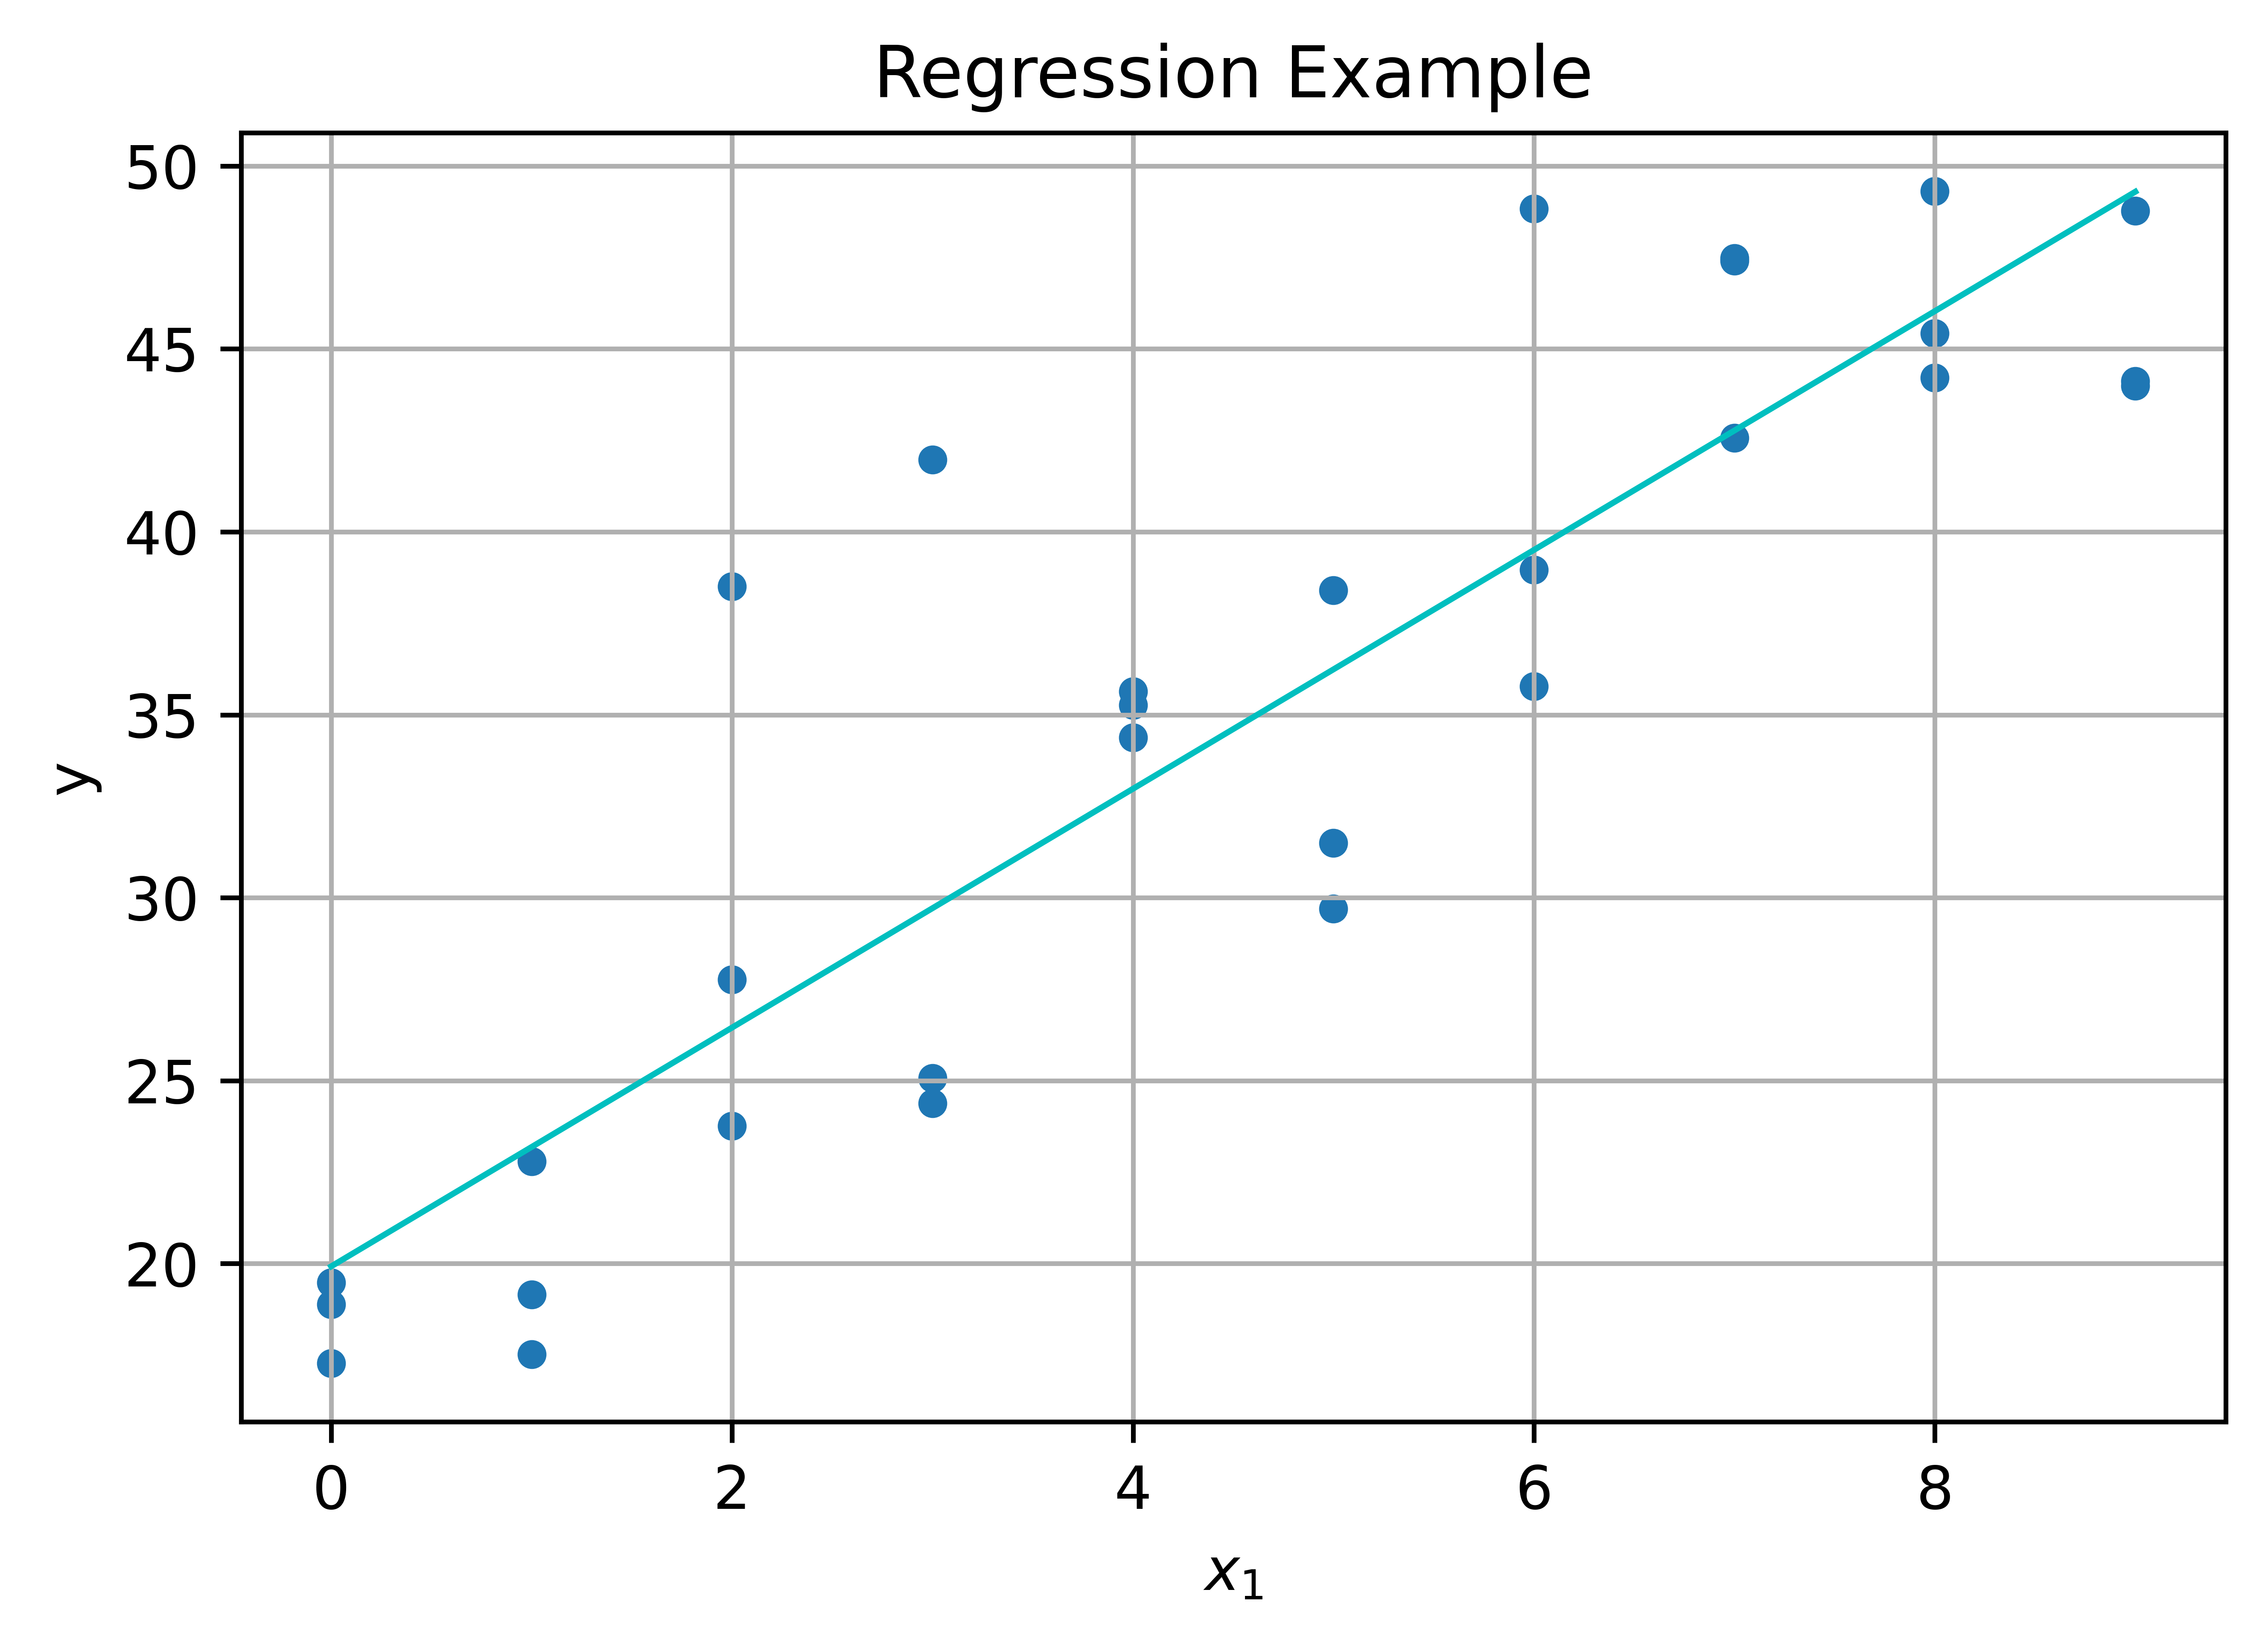
\includegraphics[width=70mm,scale=0.5]{images/regression_images/Regression_Keep_Offset.png}
        
            \caption*{Our regression example.}
        \end{figure}
        
        Let's suppose we \orgg{regularize}, or shrink, our offset $\theta_0$, while keeping everything else the same:
        
        \begin{figure}[H]
        \centering
            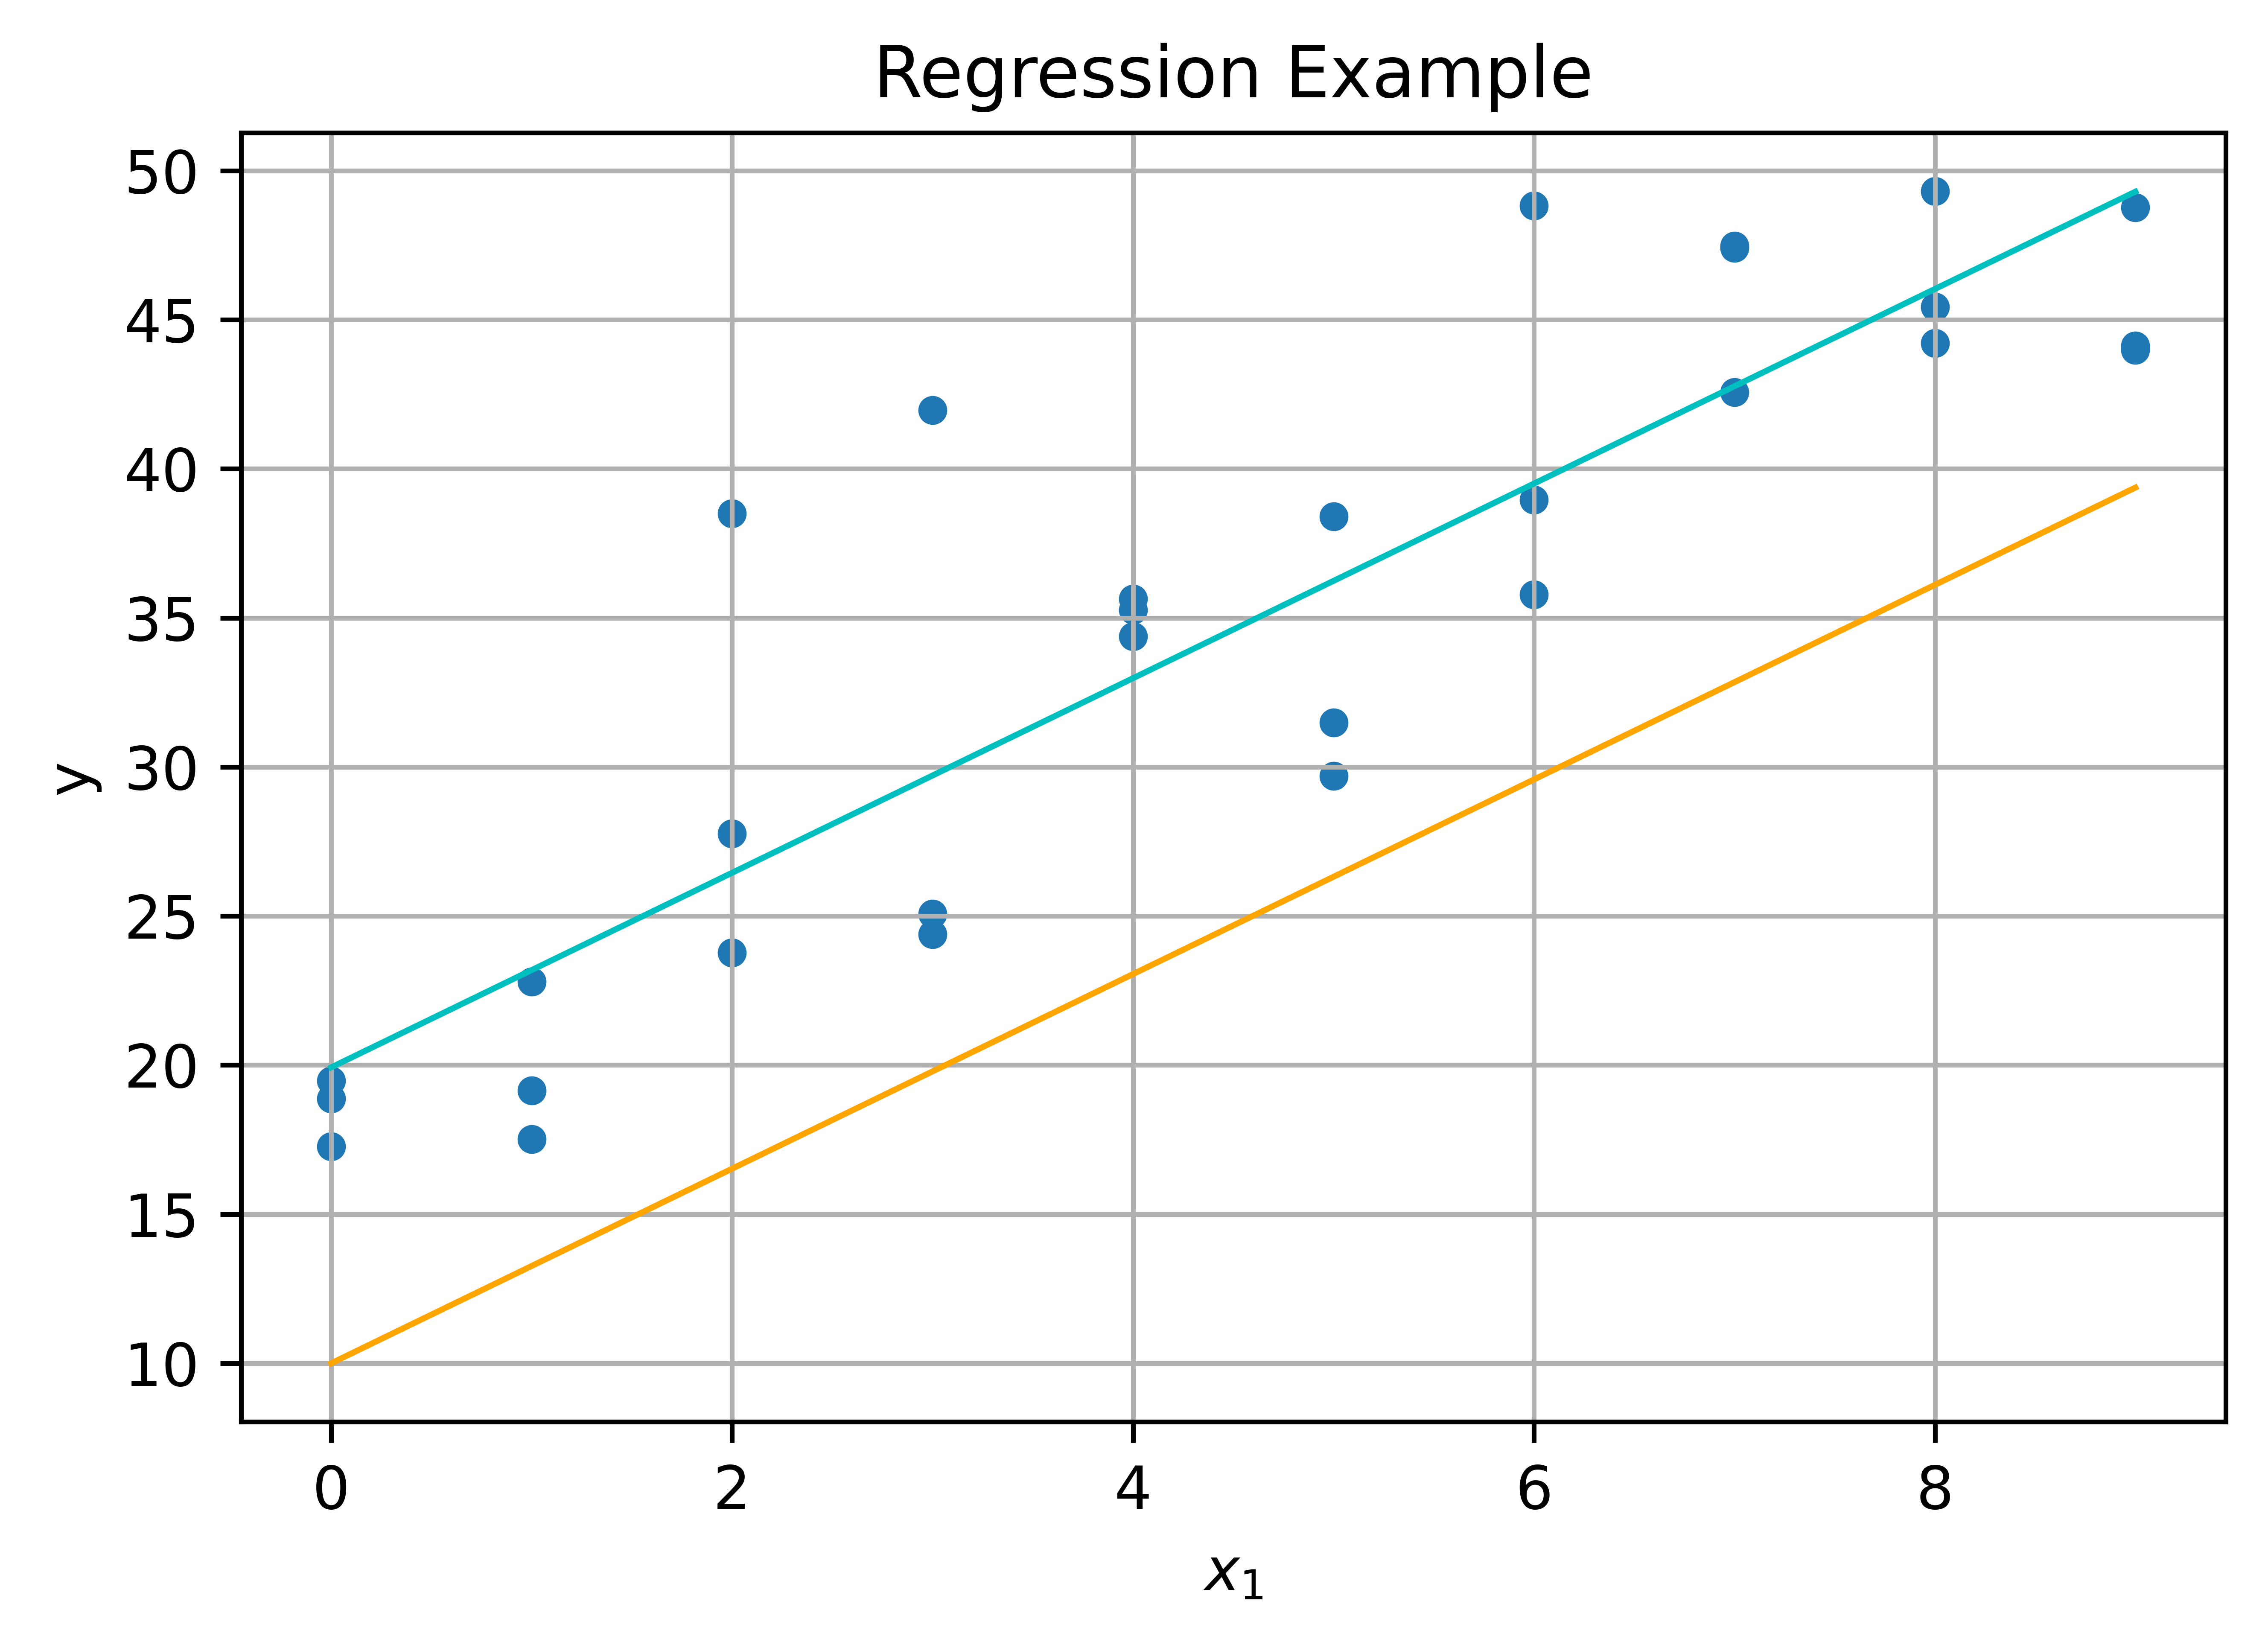
\includegraphics[width=70mm,scale=0.5]{images/regression_images/Regression_Remove_Offset.png}
        
            \caption*{Reducing our offset pulls our line further away from all of our data! This is a serious problem.}
        \end{figure}
        
        This shows that we \textbf{need} our offset! 
        
        \begin{itemize}
            \item We use it to \purp{shift} our hyperplane around the space: otherwise, otherwise, it's difficult to fit data \gren{far} from the origin.
                \note{Imagine that we have three data points at $(1, 1001)$, $(2, 1002)$, and $(3, 1003)$.
                
                \phantom{}
                
                It's clear that our data is offset by roughly 1000: we need $\theta_0$ to address this.}\\
        \end{itemize}
        
        \begin{concept}
            $\theta_0$ gives us a baseline for the \gren{size} of our output values.

            \begin{itemize}
                \item If we reduce $\theta_0$, all of our outputs will be reduced equally: they'll be \purp{less accurate.}
            \end{itemize}
        \end{concept}


    \pagebreak

    \subsection{Ridge Regression Solution}

        Now, we have our regression loss function, 

        \begin{equation}
            J(\Theta) = 
                        \frac{1}{n}  \sum_{i=1}^n 
                        \left( 
                            \underbrace{
                                \red{(\theta^T \ex{x}{i}  
                                + \theta_0)}
                            }_{guess}
                            - \underbrace{
                                \blu{\ex{y}{i}} 
                            }_{answer}
                        \right)^2 
                        + 
                        \underbrace{
                            \pur{ \lambda \norm{\theta}^2 }
                        }_{Regularizer}
        \end{equation}

        Which we can express in matrix form:
            \note{We're gonna cheat a bit, and ignore $\theta_0$.

            \phantom{}
            
            One way to do this is to subtract a constant from every value in $Y$, so that the data is centered on $y=0$: you don't \textit{need} an offset $\theta_0$.

            \phantom{}
            
            But in some problems, we might just include $\theta_0$ in $\theta$, to make our problem simpler, even though we're accidentally regularizing $\theta_0$.}

        \begin{equation}
            J(\theta) = \frac{1}{n}
                    \Big( \red{ \theta^T X - Y } \Big)
                    \Big( \red{  \theta^T X - Y } \Big)^T
            + 
            \pur{\lambda \theta^T \theta}
        \end{equation}

        We can now \gren{optimize} this for $\theta$. We'll do some matrix calculus, omitting the steps here:

        \begin{equation}
            \nabla_{\theta}J = 
            \frac{2}{n}
                    \red{ \Xt^T }
                    \Big( \blu{  \Xt \theta - \Yt } \Big)
            + 
            \pur{2\lambda \theta} = 0
        \end{equation}

        Finally, we \orgg{solve} (using some linear algebra -- multiplying by inverses, distributive property, add/subtracting, etc.):\\

        \begin{kequation}
            The \purp{solution} to the \vocab{ridge regression} problem allows us to find the \gren{optimal} model $\theta^*$.

            \begin{equation*}
                \theta^* = \Big ( \red{\Xt^T \Xt} + \blu{n \lambda I} \Big)^{-1} \org{\Xt^T \Yt}
            \end{equation*}

            or, in our original notation:

            \begin{equation*}
                \theta^* = \Big ( \red{X X^T} + \blu{n \lambda I} \Big)^{-1} \org{XY^T}
            \end{equation*}

            Where $I$ is the $(d \times d)$ identity matrix.
        \end{kequation}

            \note{Review: an identity matrix is a square matrix with 1's on its diagonal, and 0's everywhere else. 
            
            \phantom{}
            
            In general, $AI=IA=A$.}


    \pagebreak

    \subsection{Invertibility}

        This solution is great! We just have one problem:

        \begin{itemize}
            \item It requires that our \purp{inverse} of $(XX^T+n\lambda I)^{-1}$ exists.
        \end{itemize}

        Thankfully, this is true so long as $\lambda>0$!\\

        \begin{concept}
            If $\lambda>0$, we can be sure that $(XX^T+n\lambda I)$ has an \purp{inverse}.

            \begin{itemize}
                \item And thus, we have a \gren{unique solution} to $\theta$ for our \vocab{ridge regression problem.}
            \end{itemize}
        \end{concept}

        You \redd{do not need to know} the linear algebra that justifies this statement. You just need to know that it's true.
            \note{The short version of the justification is:

            \phantom{}
            
            $XX^T$ is positive semi-definite: $v^T XX^T v \geq 0$. 

            \phantom{}
            
            If you add positive elements on the diagonal ($A=XX^T+n \lambda I$), then you can only increase $v^T A v$: now it's $v^T A v > 0$.

            \phantom{}

            Thus, $(XX^T+n\lambda I)$ is positive definite: this means it has an inverse.

            \phantom{}

            If that doesn't make any sense, don't worry about it.}

        This, by the way, presents one more justification for regularization:\\

        \begin{concept}
            Another benefit of \vocab{regularization} is that we can \purp{always} find an \gren{analytical solution} for $\theta$.

            \begin{itemize}
                \item $\Big ( \red{\Xt^T \Xt} + \blu{n \lambda I} \Big)$ is invertible, thus, we can compute 

                \begin{equation*}
                    \theta^* = \Big ( \red{X X^T} + \blu{n \lambda I} \Big)^{-1} \org{XY^T}
                \end{equation*}
            \end{itemize}
        \end{concept}

        Sometimes, we call non-invertible matrices \orgg{singular}.\\

        \begin{definition}
            All of the following statements about square matrix $A$ are equivalent:

            \begin{itemize}
                \item $det(A)=0$.
                \item $A$ has \redd{no inverse}.
                \item $A$ is \gren{singular}.
                \item $A$ is \purp{not full rank}.
            \end{itemize}

            
        \end{definition}

        A few more definitions of singular:

        \begin{itemize}
            \item $A$ has at least one eigenvalue of 0.
            \item $A$ has linearly dependent rows and columns.
            \item $Ax=0$ has a solution other than $x=0$.
                \note{Sometimes, you say this as, "$Ax=0$ has a non-trivial solution".}
        \end{itemize}

        Relevant for regularization: a positive definite matrix is nonsingular.
            \note{The converse (a nonsingular matrix is positive definite) is not necessarily true!}

    \phantom{}

    \subsection{Uniqueness of $\theta^*$}

        This seems suspicious: why on earth would \redd{regularizing} $\theta$ allow us to find a solution?

        \begin{itemize}
            \item In order to understand this, we need to understand \gren{what happens} when $XX^T$ is \purp{singular}.
        \end{itemize}

        \phantom{}

        If $XX^T$ isn't full rank, that means that $X$ \purp{isn't full rank}, either.
            \note{Showing that this is true is more a linear algebra problem than an ML problem, so we'll defer it here.}


        What does this mean? Let's consider an example in 1d: we'll compare a "full rank" version, to one that isn't full-rank.

        \begin{figure}[H]
        \centering
            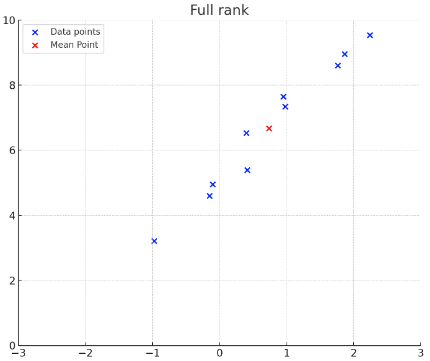
\includegraphics[width=70mm,scale=0.5]{images/regression_images/full_rank.png}
            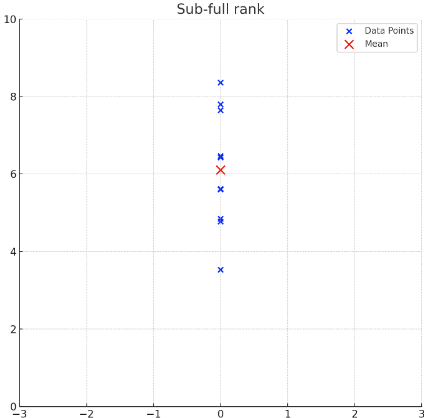
\includegraphics[width=60mm,scale=0.5]{images/regression_images/sub_full_rank.png}
            \caption*{Typically (left plot), we expect our data to be \gren{full rank}: our input space is 1-D, our input data occupies  1-D.

            \phantom{}
            
            But sometimes (right plot), we might have data which is \purp{less than full rank}: in this case, the input data is 0-D: only occupying $x=0$.}
        \end{figure}

        Sure, this data looks weird, but why is this problematic? Because it creates \orgg{multiple optimal solutions}:

        \begin{figure}[H]
        \centering
            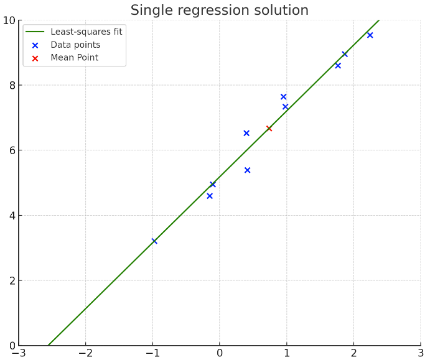
\includegraphics[width=70mm,scale=0.5]{images/regression_images/full_rank_regression.png}
            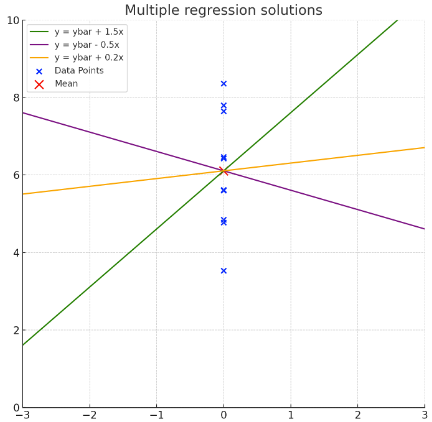
\includegraphics[width=60mm,scale=0.5]{images/regression_images/sub_full_rank_regression.png}
            \caption*{Our "full rank" (left plot) data has one optimal solution.
            
            Our "sub-full rank" (right plot) data has many!}
        \end{figure}

        This is the real reason why, if $XX^T$ isn't invertible, we can't find an analytical solution: there are actually \purp{many} possible solutions!\\

        \begin{concept}
            If $XX^T$ isn't invertible, we \purp{cannot} use our formula to find an analytical (formula-based) \gren{solution} for $\theta$.

            \begin{itemize}
                \item That's because there are \orgg{many optimal solutions}.

                \item In fact, there are \gren{infinitely many of them!}
            \end{itemize}
        \end{concept}

            \note{We call this kind of problem \purp{collinearity}: our input data sit on a lower-dimensional "linear" surface.}

        We can see this in higher dimensions too: below, we have a 2-d input space (3-d plot), but our inputs only occupy a \purp{line}.

        \begin{figure}[H]
        \centering
            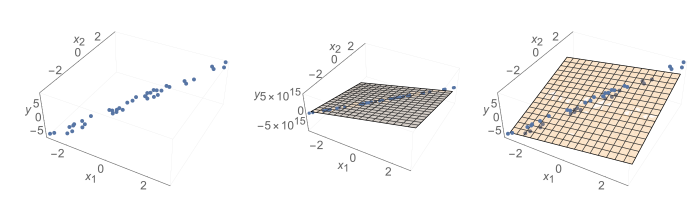
\includegraphics[width=120mm,scale=0.5]{images/regression_images/Regularizer_Multiple_Solutions.png}
        
            \caption*{There are many possible planes that go through that line: each of these is an \gren{equally good} solution for regression.}
        \end{figure}

        \phantom{}

        We don't have this problem if we use regularization: among all of our \gren{equivalent} options, we just pick the one with the \purp{minimal} $||\theta||$.

        \begin{figure}[H]
        \centering
            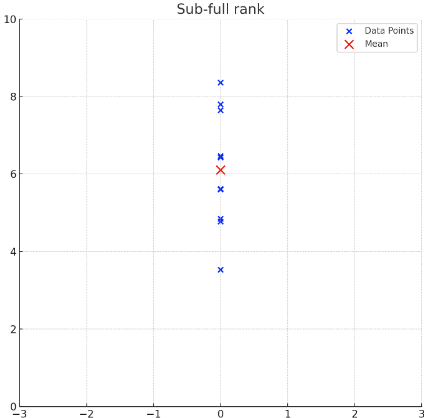
\includegraphics[width=60mm,scale=0.5]{images/regression_images/sub_full_rank.png}
            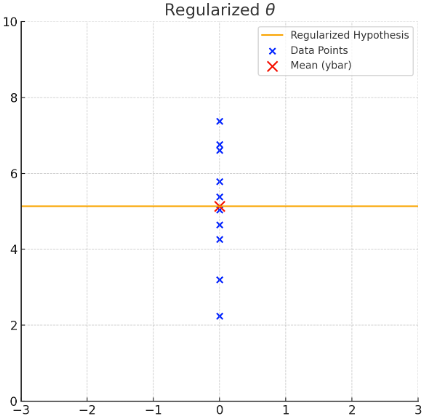
\includegraphics[width=60mm,scale=0.5]{images/regression_images/singular_data_regularized.png}
            \caption*{Now, we have one solution: we can get this analytically!}
        \end{figure}
            

        \pagebreak

    \subsection{Error Amplification}

        Surely, this is a really rare situation: our data typically won't line up \gren{perfectly}.

        \begin{itemize}
            \item Maybe, but that's part of the problem: let's see what happens if our data is \purp{not} perfectly aligned. We say that $XX^T$ is \vocab{ill-conditioned} or "nearly singular".\\
        \end{itemize}

        \begin{definition}
            We call a matrix \vocab{ill-conditioned} or \purp{nearly singular} if it is very close to a singular/non-invertible matrix.
        \end{definition}

            \note{You can compute whether a matrix is ill-conditioned using something called a "condition number", but we'll omit that point.}

        \begin{figure}[H]
        \centering
            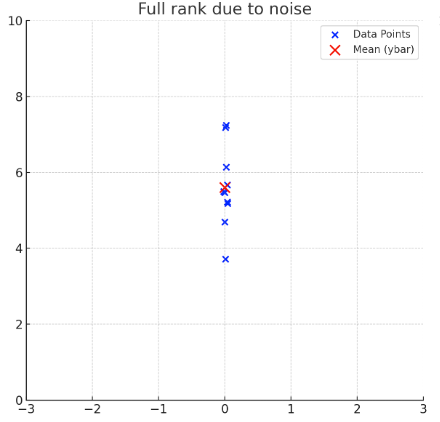
\includegraphics[width=60mm,scale=0.5]{images/regression_images/noisy_full_rank.png}
            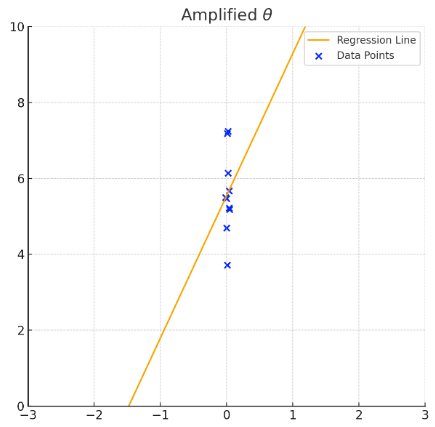
\includegraphics[width=60mm,scale=0.5]{images/regression_images/amplified_theta.png}
            \caption*{Our data has a \gren{large slope} now! This is a problem: $x$ has \purp{no effect} on $y$, we just added a little noise to the $x$-axis.}
        \end{figure}

        Our model notices, "\gren{very small} change in $x$, \purp{moderate} change in $y$", and assumes the slope $\theta$ should be \orgg{large}.
            \note{Another way to see this: technically, if you wanted to draw a line through the data, you'd draw a vertical line: "infinite" slope.}

            \begin{itemize}
                \item This is wrong: our change in $y$ isn't actually explained by $x$, it's explained by some "\purp{randomness}" in the output (which is common in real data).\\
            \end{itemize}

        \begin{concept}
            One problem with data that \textit{almost} falls on a line, is \vocab{error amplification}.

            \begin{itemize}
                \item If $x_i$ varies by a small amount, while $y$ varies by a larger amount, our model may assume $\theta_i$ is \purp{very large}.

                \item That means that, if you had a much larger $x_i$ value, the model will predict $y$ is \orgg{way larger}.
            \end{itemize}

            Thus, our error gets \purp{amplified} as we move further away.
        \end{concept}

            \note{Sometimes, you might hear people mention "numerical instability" of the inverse when a matrix has a small determinant: these are, mathematically, the same problem.
            
            \phantom{}
            
            If $det(A)=0.01$, then $det(A^{-1})=100$. The closer you are 0, the more dramatic the effect.}


        If our problem is that $\theta$ is too large, then we can solve this problem by regularizing $\theta$.

        \begin{figure}[H]
        \centering
            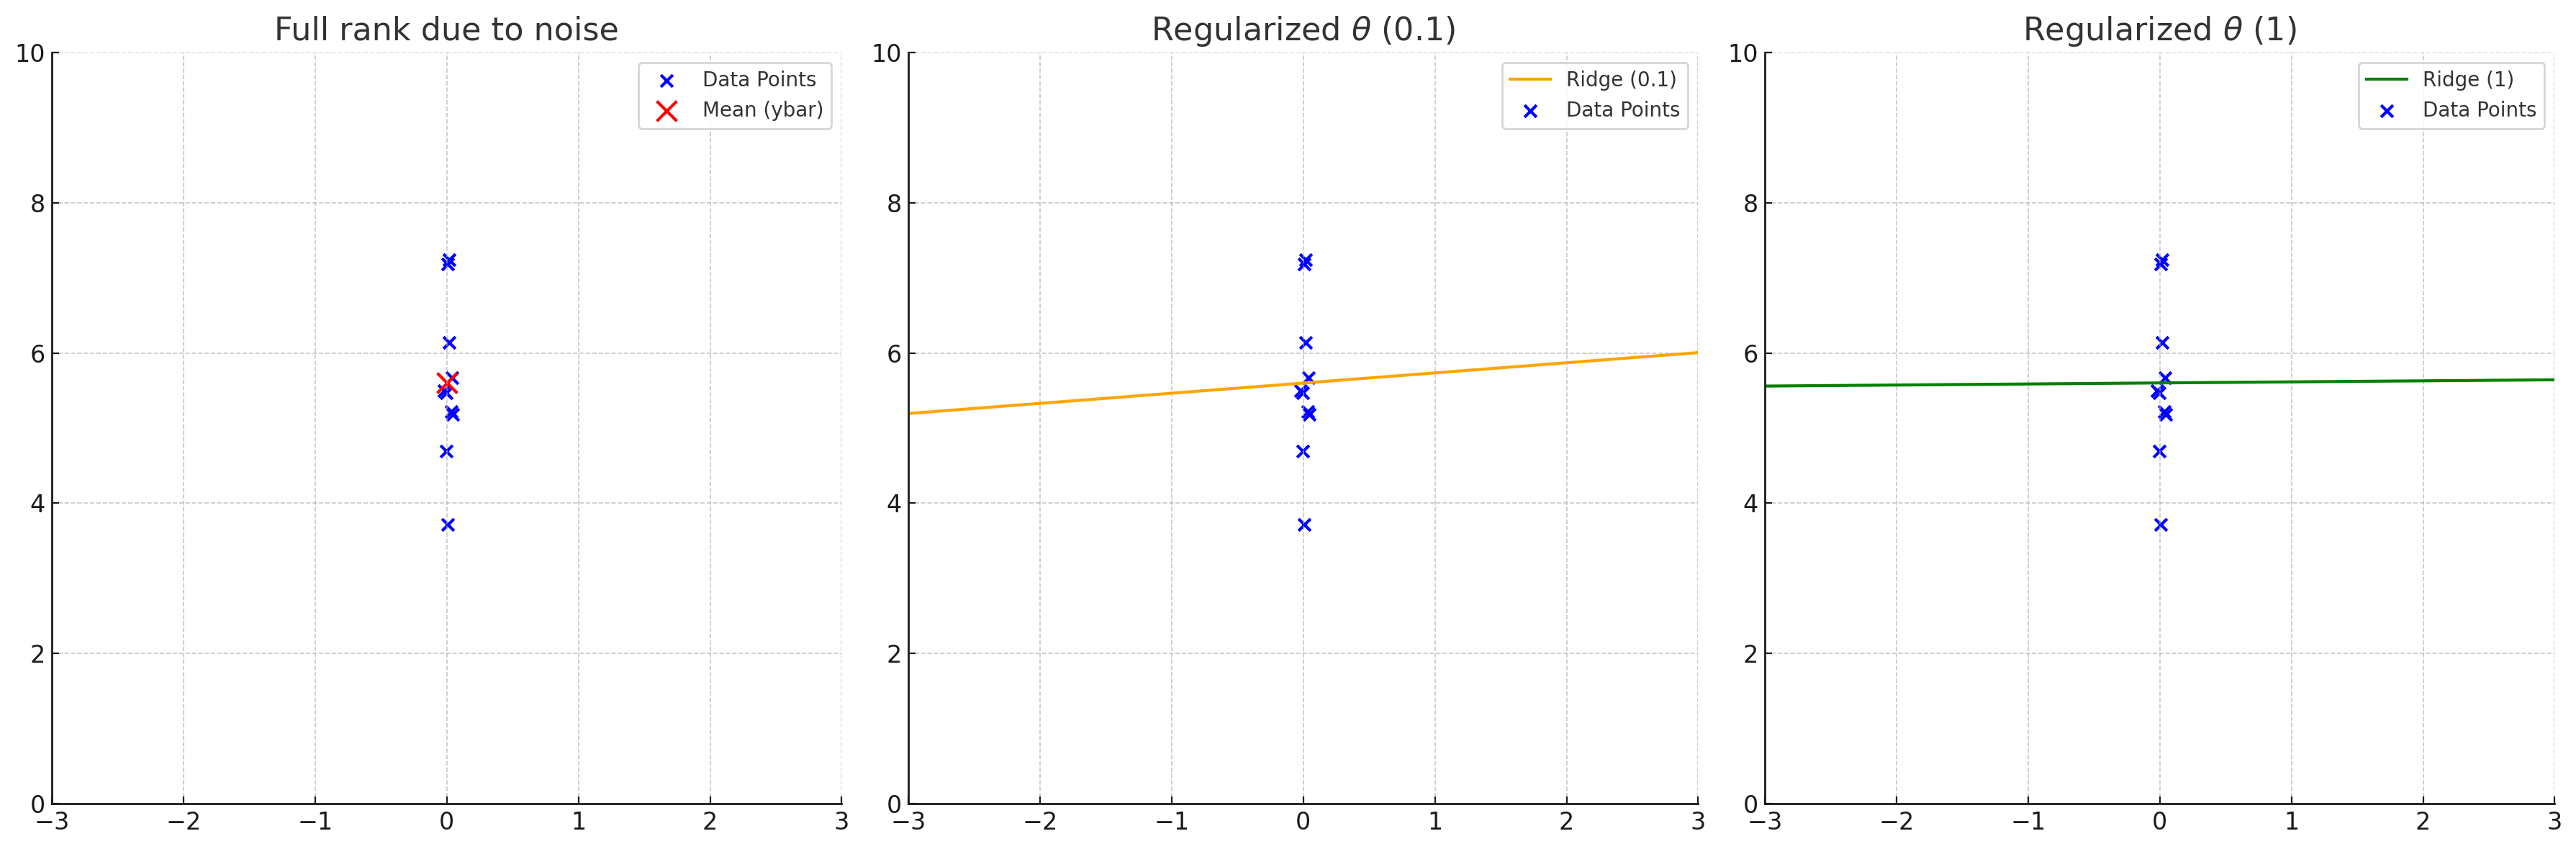
\includegraphics[width=150mm,scale=0.5]{images/regression_images/full_rank_noise_regularized.png}
            \caption*{With $\lambda=0.1$, our slope is already much less sharp. with $\lambda=1$, we end up with (mostly) the same solution as we did in the singular case.}
        \end{figure}

        \begin{concept}
            \vocab{Ridge Regression} helps \purp{improve} our model by
            
            \begin{itemize}
                \item Making our model more \purp{general} and resistant to \gren{overfitting}
                \item Making sure \gren{solutions} are \purp{unique}
                \item Keeping our matrix $XX^T$ \purp{invertible}, so we can find a \gren{solution}.
            \end{itemize}
        \end{concept}

        \phantom{}

        \subsection{Error Amplification Example (\redd{Optional})}

            Here's a very simple computational example:

            \begin{itemize}
                \item \miniex Suppose that two inputs are \orgg{almost exactly the same}: $x_1^{(1)}=0$, and $x_1^{(2)}=0.01$. 
                \item But, the outputs are \purp{somewhat} different.  The outputs are $y^{(1)}=25$, $y^{(2)}=26$.
            \end{itemize}

            If we assume \textbf{all} of the change in the output is a result of the the \textbf{input}, then it looks like a \gren{tiny} change in $x_1$ has a \purp{huge} effect on the output $y$.

            \begin{equation}
                \deriv{y}{x} = \frac{\Delta y}{\Delta x} = \frac{1}{.01} = 100
            \end{equation}
    
            This suggests that $x_1$ has a \redd{100x} effect on our output! Even though, it could just be that $x$ has small variation, and $y$ has larger variation.
    
            \begin{equation}
                100 x_1 + 25 = h(x)
            \end{equation}

            Imagine that $x_1=10$: suddenly, the prediction is 1025. That's why we call it \vocab{error amplification}: a small error near $x=0$, becomes huge as we get further away.


    

    \pagebreak
    \subsection{Regularizer justification: Prior Knowledge (\redd{Optional})}

        One more way to justify our regularizer applies to a lot of broader statistics: the concept of a \vocab{prior belief}.

        \begin{itemize}
            \item Suppose we have prior expectations about what our model should look like: based on theory, or prior experience.

            \item We might consider a model \textbf{more different} from that past one, $\Theta_{\text{prior}}$, to be \textbf{suspicious}, and less likely to be good.
        \end{itemize}

        So, we can \purp{punish our model} for being too different from that expectation.

        \begin{itemize}
            \item This makes our model more \gren{conservative}: it avoids creating a very "extreme" model, without strong justification from the training data.
                \note{Our data has to "convince" us that it's worth trying a different model.}\\ 
        \end{itemize}
       
        \begin{concept}
            If we have a \purp{prior} hypothesis $\Theta_{\text{prior}}$ to work with, we might improve our \purp{new} model by encouraging it to be \gren{closer} to the old one.
            
            \begin{equation*}
                R(\Theta)= \norm{ \Theta - \Theta_{\text{prior}} }^2
            \end{equation*}
            
            We measure how \gren{similar} they are using \vocab{square distance}.
            
        \end{concept}
        
        \miniex You have a \textbf{pretty good} model for \textbf{predicting} company profits, but it isn't perfect. You decide to train a \textbf{better} one, but you expect it to be \textbf{similar} to your old one.

        \phantom{}

        In our case, we \purp{don't have} a prior hypothesis $\theta_{prior}$. We have no clue of what a \gren{good solution} looks like.

        We'll take a neutral stance:

        \begin{itemize}
            \item When we know nothing, we're \orgg{equally likely} to expect $\theta_k$ to be positive, or negative. 
            \item In other words, we don't know if $x_i$ is likely to increase or decrease $y$.
        \end{itemize}

        So, our guess should average out to 0: the most likely effect is \purp{none}.

        \begin{itemize}
            \item Another way to justify this: if we pick a bunch of variables randomly, we might expect a lot of them to be \orgg{irrelevant}.
            \item \miniex Without knowing anything, we probably don't expect your birth date to affect your academic performance, positive or negatively.
        \end{itemize}

        Thus, we treat $\Theta_{\text{prior}} = \vec{0}$.\\

        \begin{concept}
            We can interpret \vocab{ridge regression} as expecting each $\theta_k$ terms to be close to 0.
            
            \begin{itemize}
                \item In other words, $\Theta_{\text{prior}}=\vec{0}$.
            \end{itemize}

            \begin{equation*}
                R(\Theta) = ||\theta-\vec{0}||^2 = ||\theta||^2 
            \end{equation*}

            This is the same formula we arrived at earlier.
        \end{concept}
        
    
\pagebreak
%%%%%%%%%%%%%%%%%%%%%%%%%%%%%%%%%%%%%%%%%%%%%%%%%%%%%%%%%%%%%%%%%%%%%%%%%%%%%%%%%%%%%%%%%%%
        
\section{Evaluating Learning Algorithms}

    Now, we have successfully developed an \textbf{algorithm} for \textbf{learning} from our data. But, did our algorithm make a \textbf{good} hypothesis? How do we do \textbf{better}?
    
    \subsection{What $\lambda$ should we choose?}
    
        There's something we ignored earlier: how do we pick the \textbf{best} value of $\lambda$? We didn't go into detail, but that value of $\lambda$ will affect our algorithm's \textbf{performance}.
        
        \begin{itemize}
            \item We mentioned that different $\lambda$ values have different \textbf{tradeoffs}, so we need to figure out which $\lambda$ value is best for our problem.
            
            \item This $\lambda$ adjusts exactly how we learn: how do we balance learning from \textbf{data} against the need to \textbf{generalize}?
        \end{itemize}
        
        So, we need to \textbf{optimize} our $\lambda$ value. Let's figure out how to go about that.
        
    \subsection{Tradeoffs: Estimation Error}
    
        High and low $\lambda$ values have benefits and drawbacks. These tradeoffs can be loosely divided into \textbf{two categories}.
        
        When we generalize, we're trying to avoid \vocab{estimation error}: we incorrectly guess the overall distribution we're trying to fit. We \textbf{estimate} poorly if we \textbf{generalize} poorly.\\
        
        \begin{definition}
            \vocab{Estimation error} is the error that results from poorly \gren{estimating} the \purp{solution} we're trying to find. 
            
            This can be caused by \gren{overfitting}, getting a bad (\purp{unrepresentative}) sample, or not having enough \gren{data} to come to conclusion.
        \end{definition}
        
        \miniex Let's try a regression problem, but we'll use only 4 points to make our plot.
        
        \begin{figure}[H]

            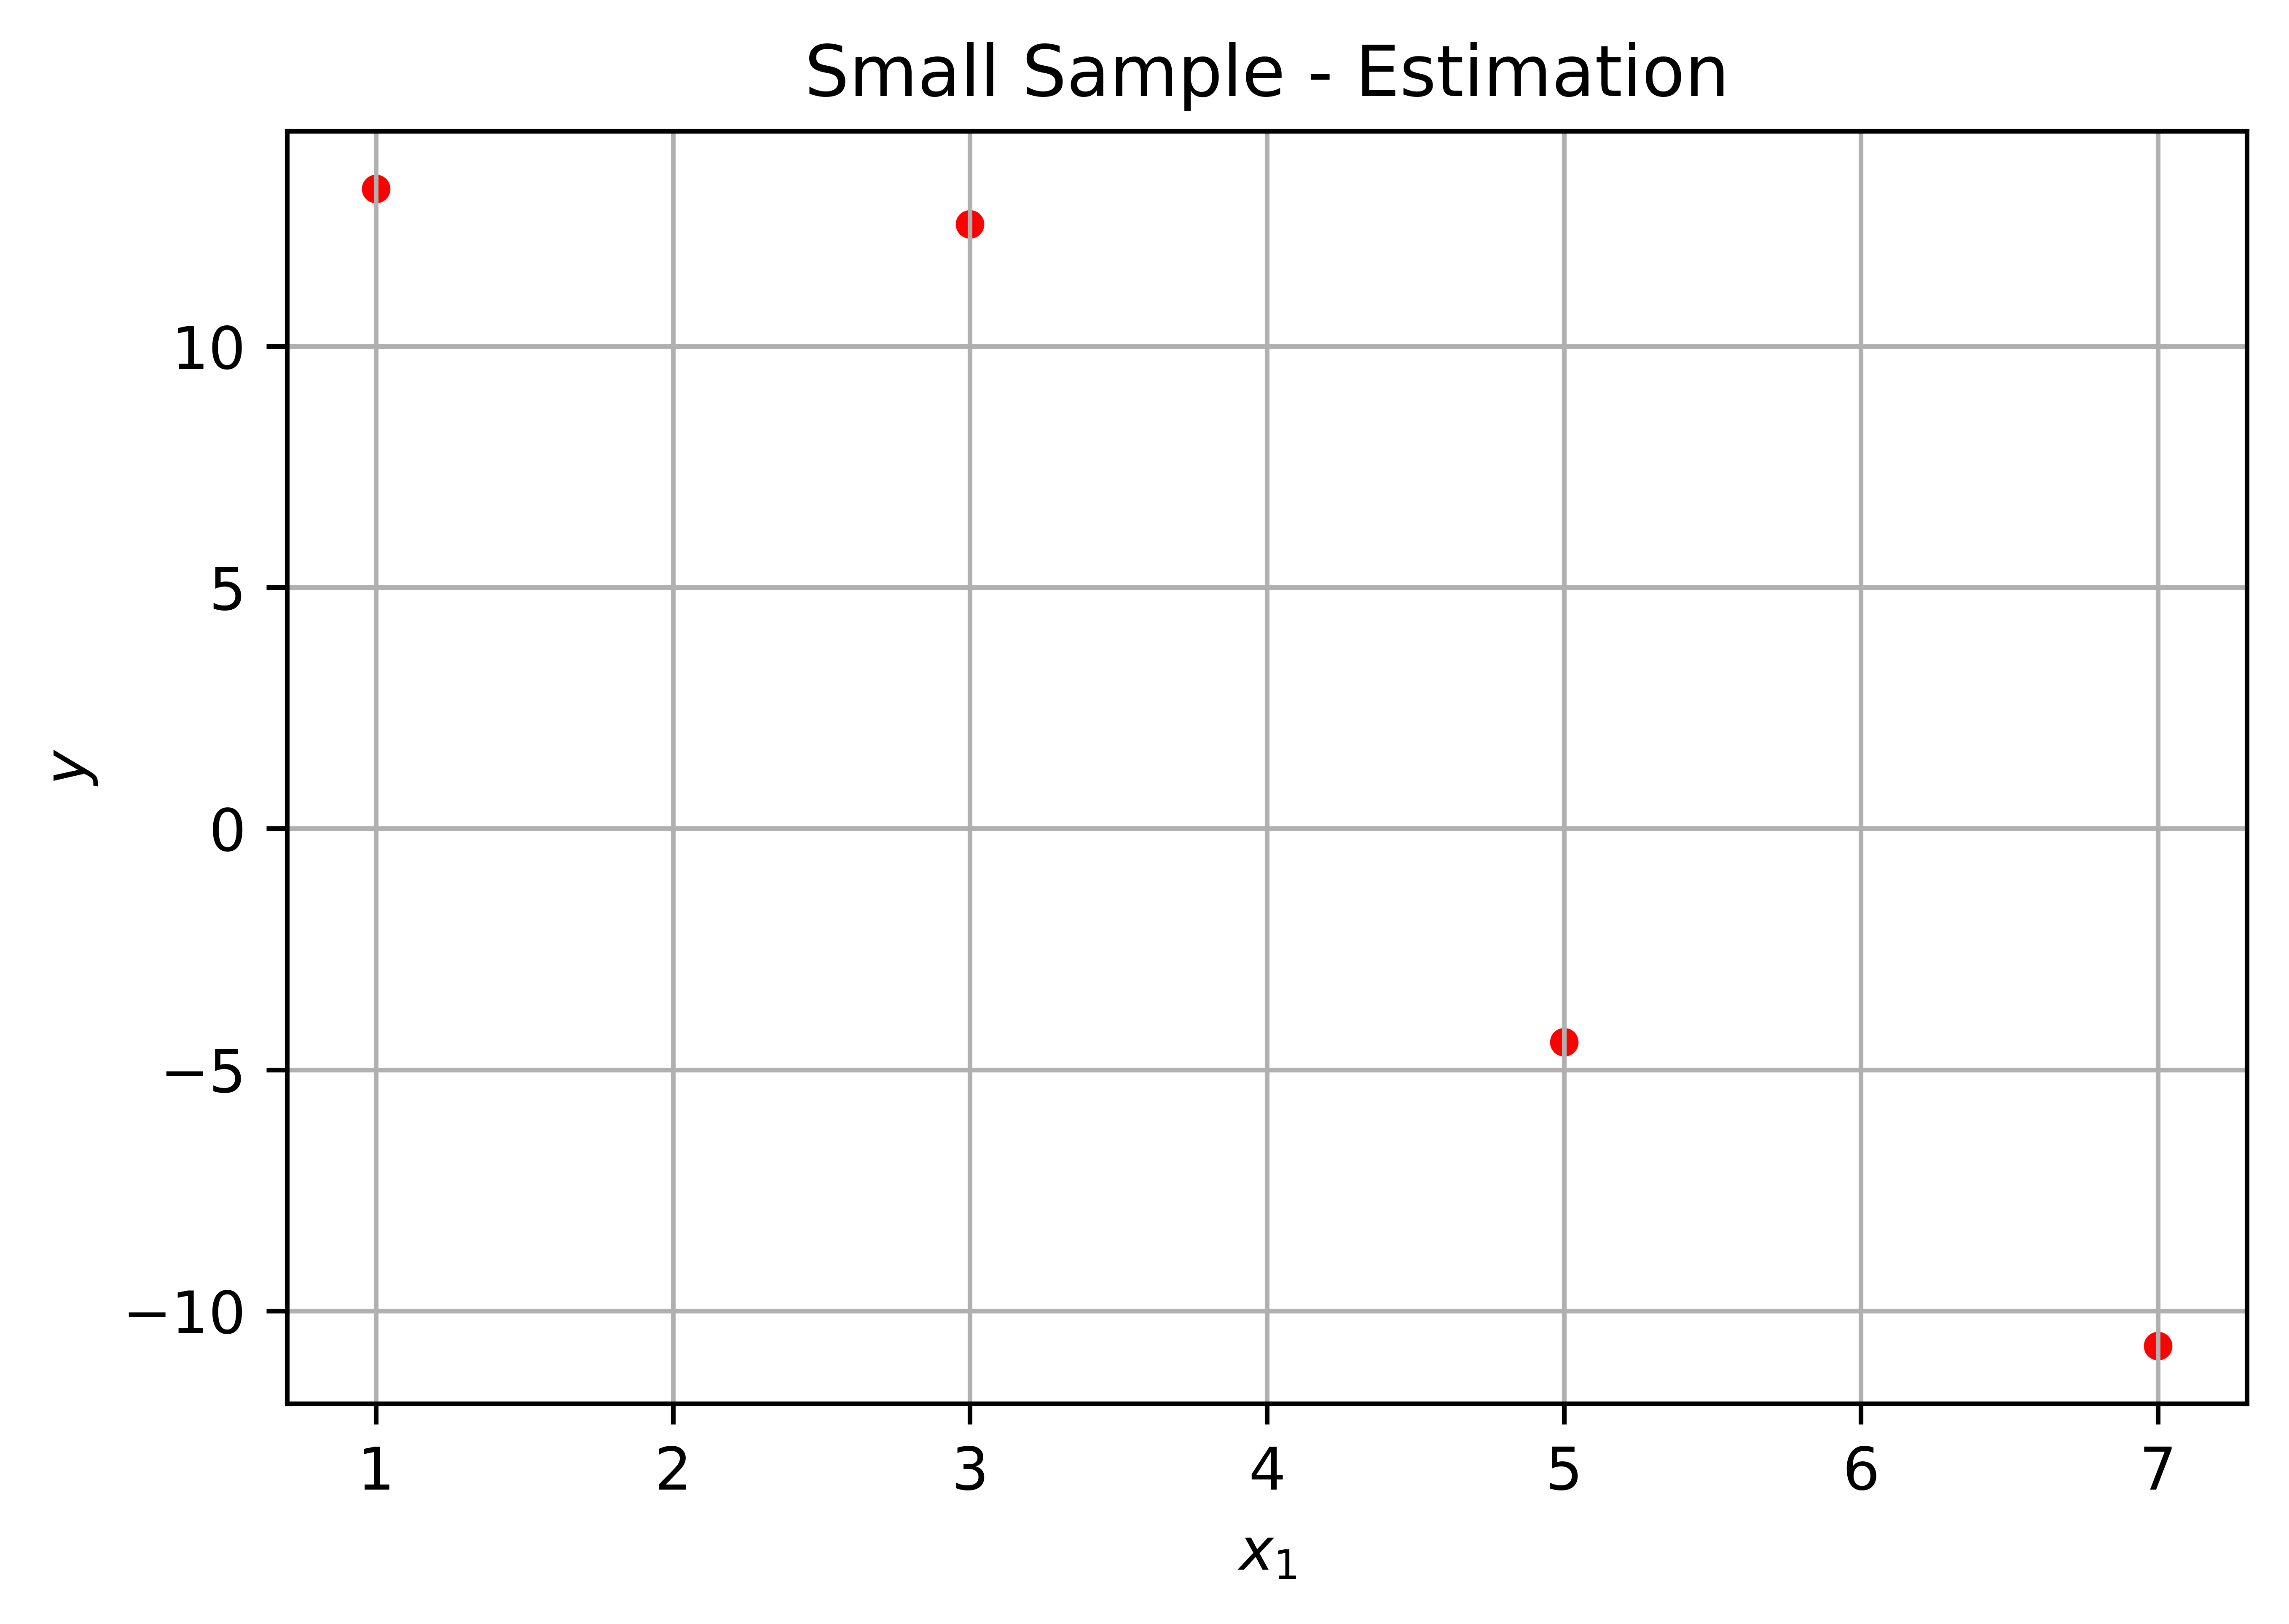
\includegraphics[width=70mm,scale=0.5]{images/regression_images/Estimation_Limited_Sample.png}

            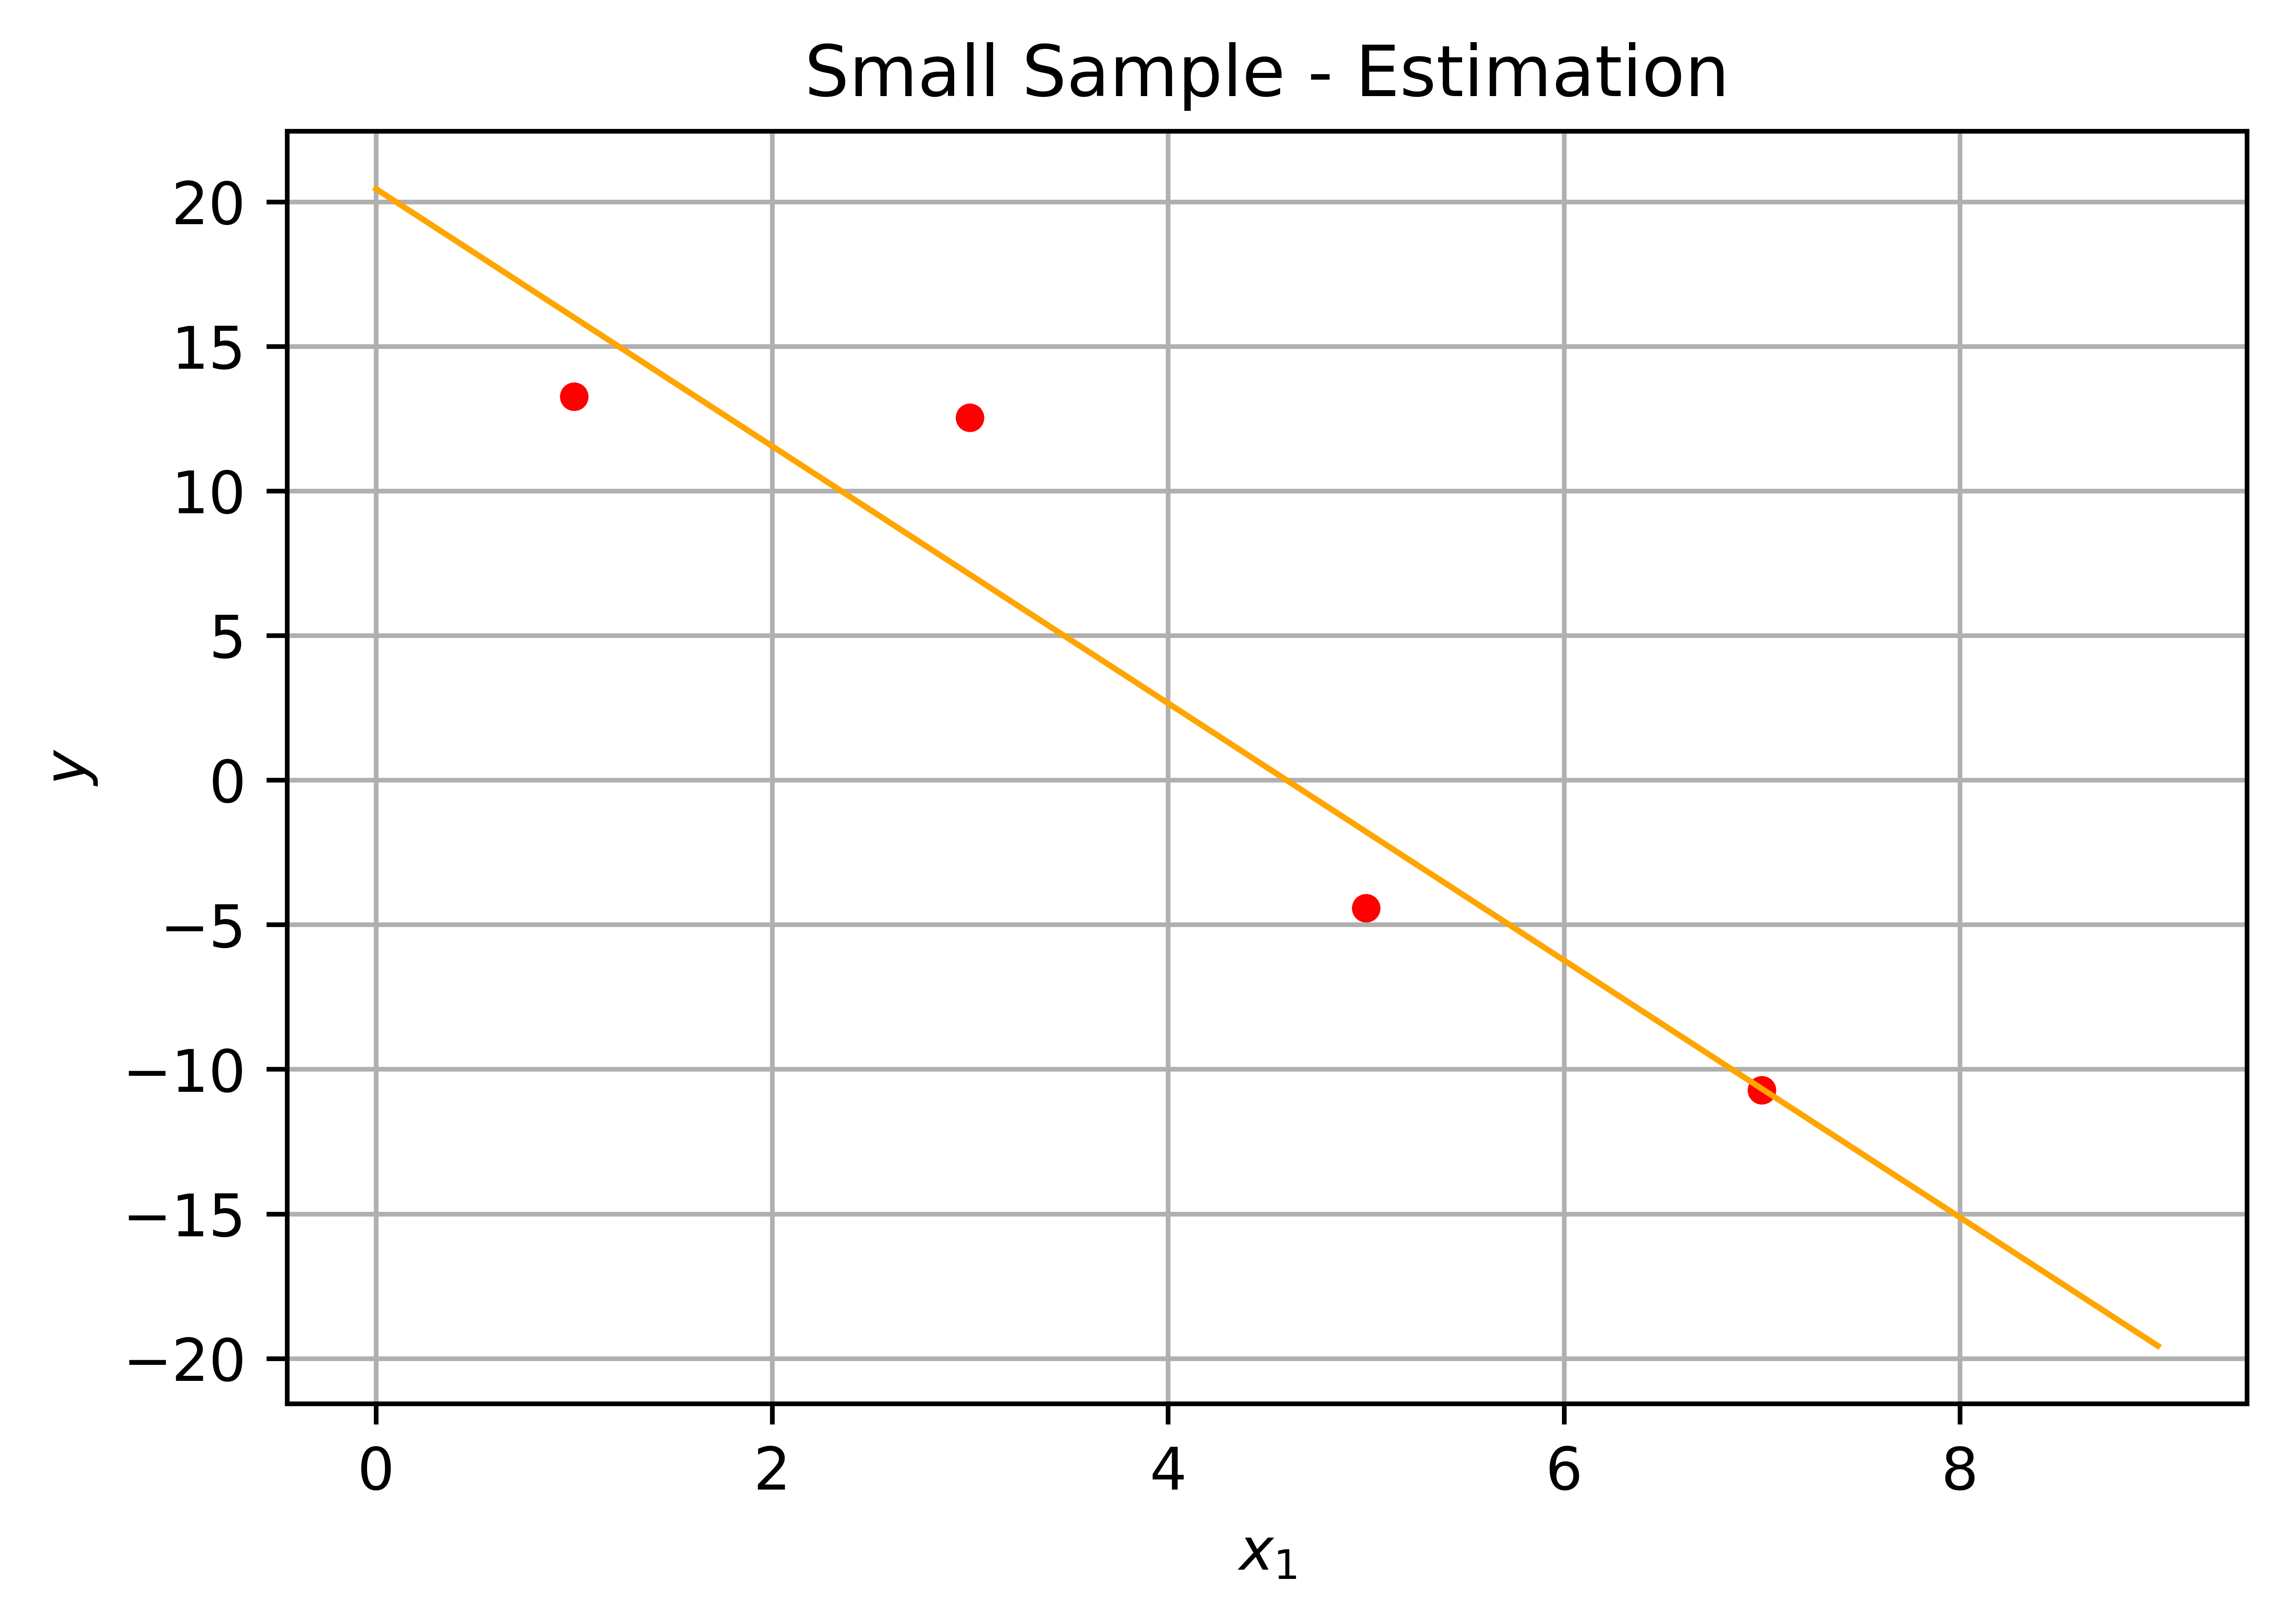
\includegraphics[width=70mm,scale=0.5]{images/regression_images/Estimation_Limited_Sample_Regression.png}
        
            \caption*{This is the regression solution we get based on our small dataset.}
        \end{figure}
        
        We might be suspicious. One way to reduce \textbf{estimation error} is to increase our number of data points (though this isn't always an option, or sufficient!)
        
        \begin{figure}[H]

                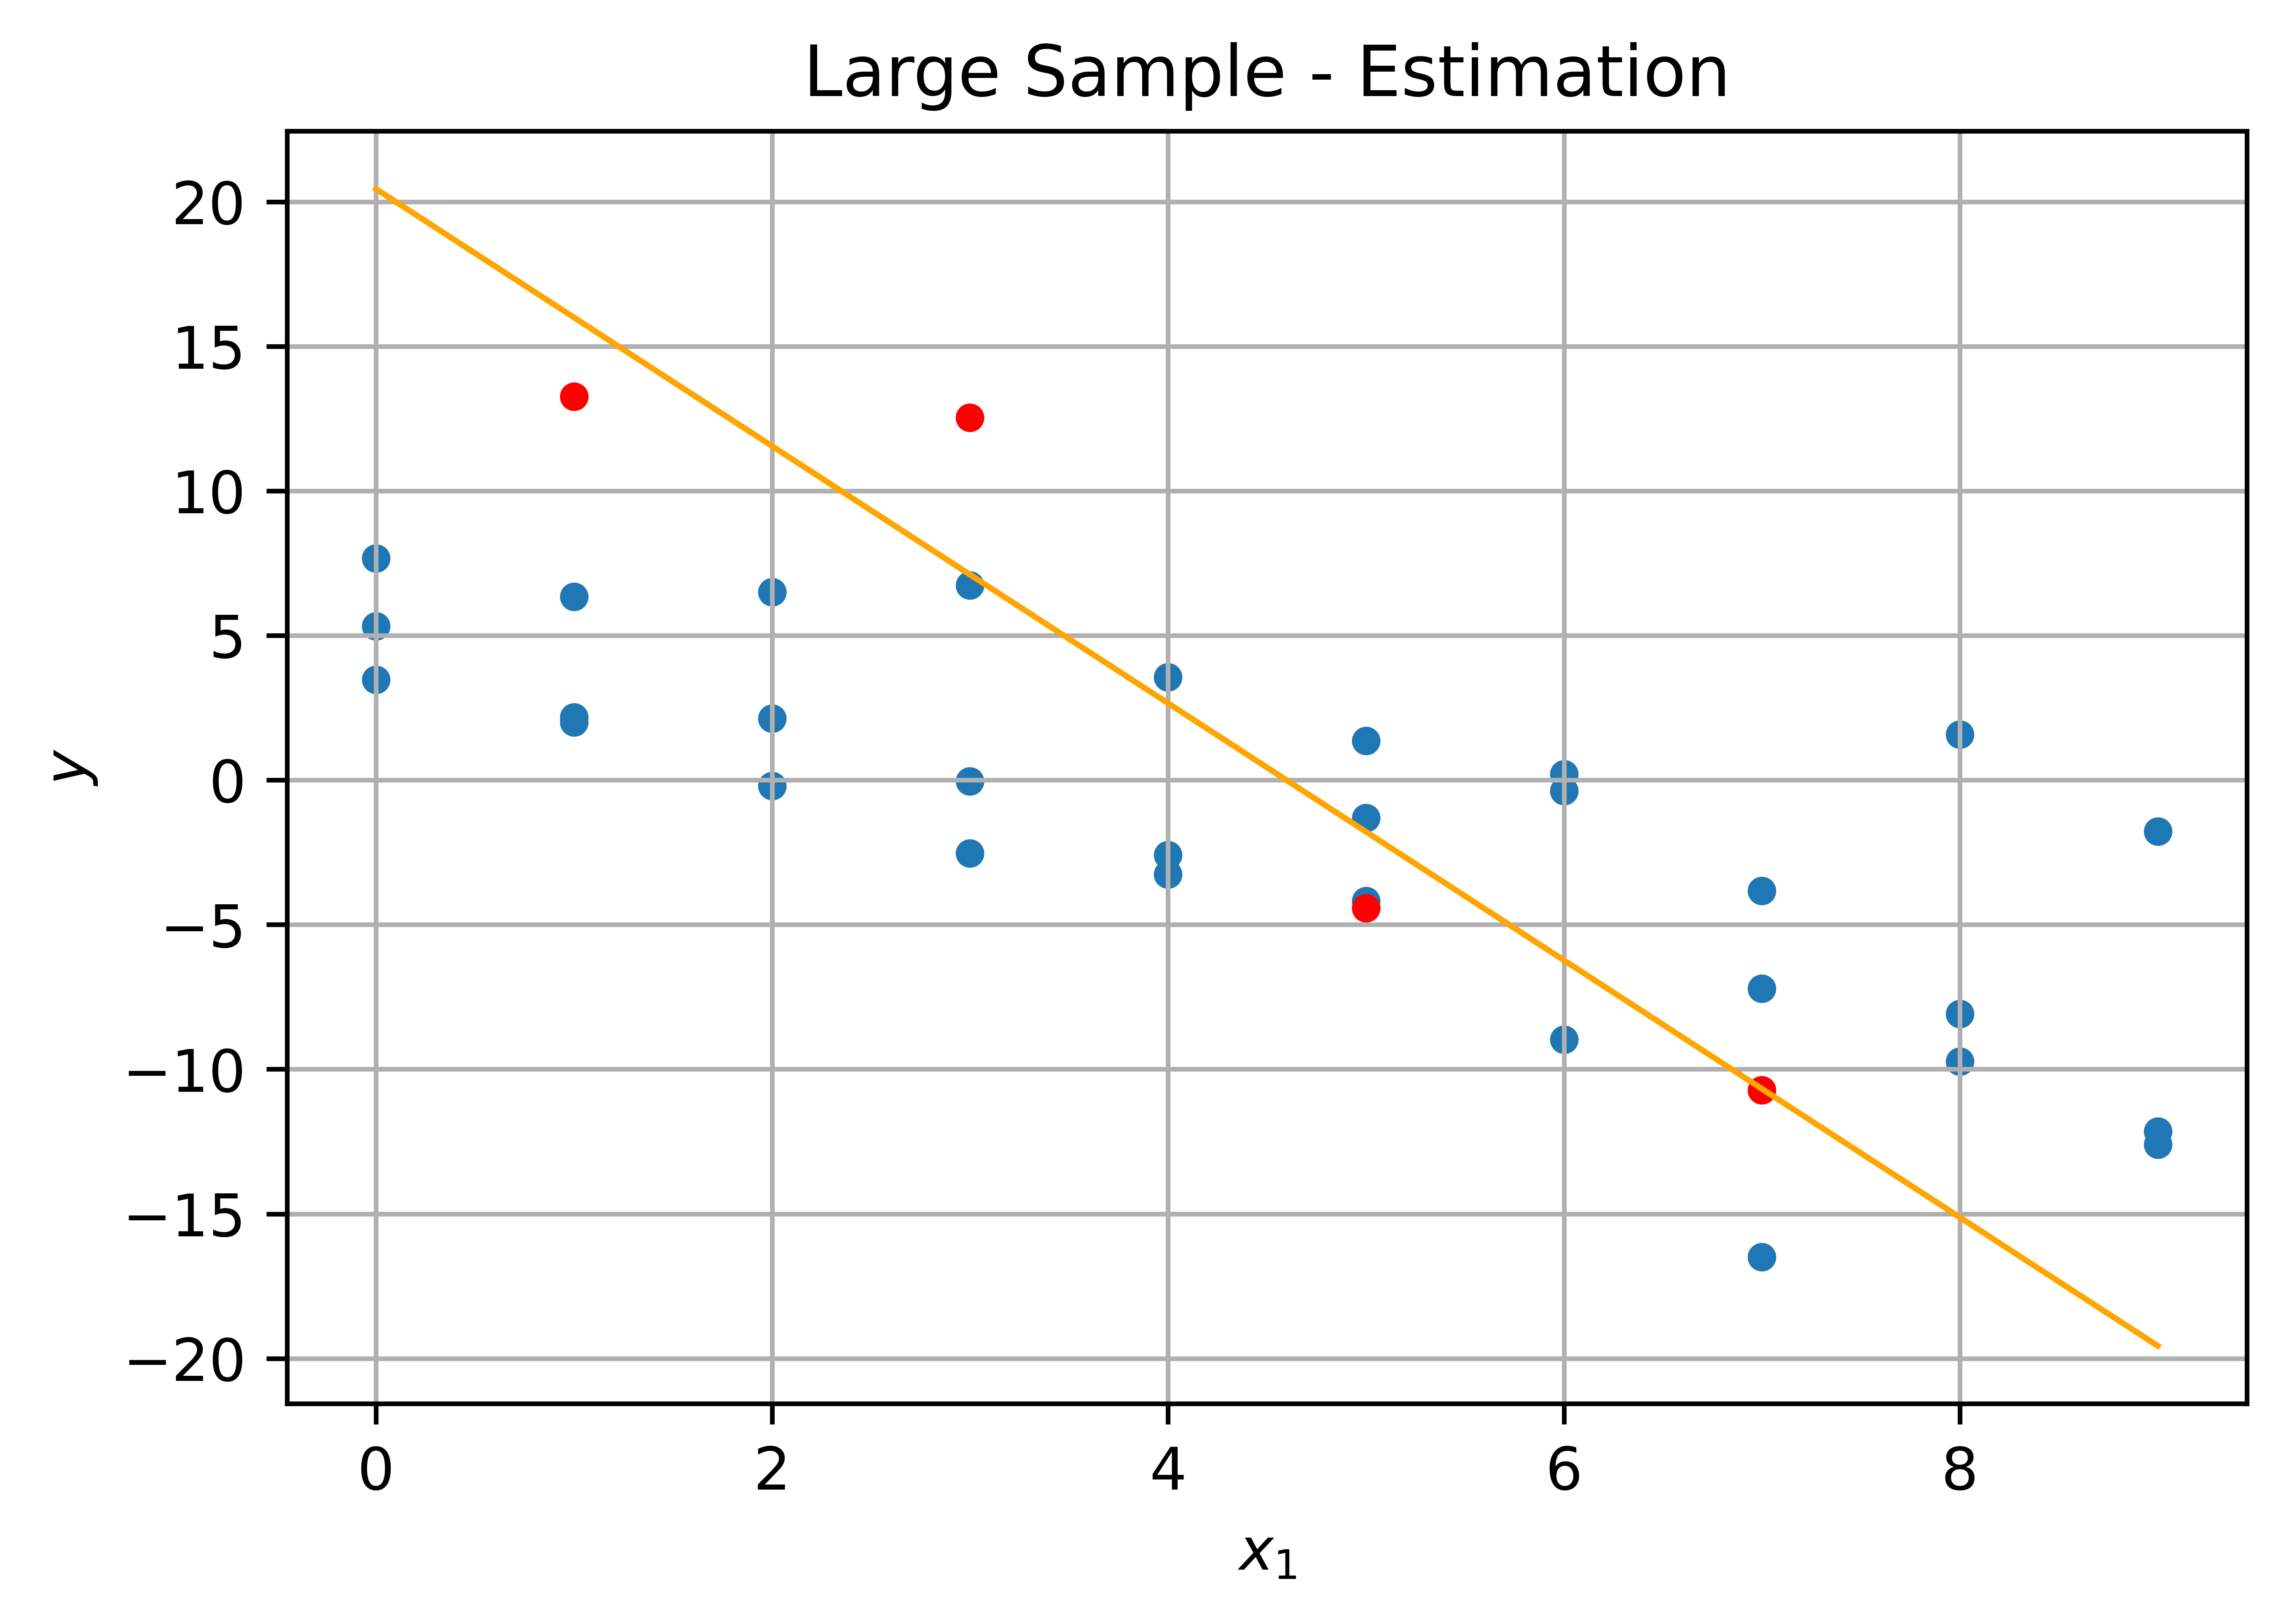
\includegraphics[width=70mm,scale=0.5]{images/regression_images/Estimation_Full_Sample.png}
                
                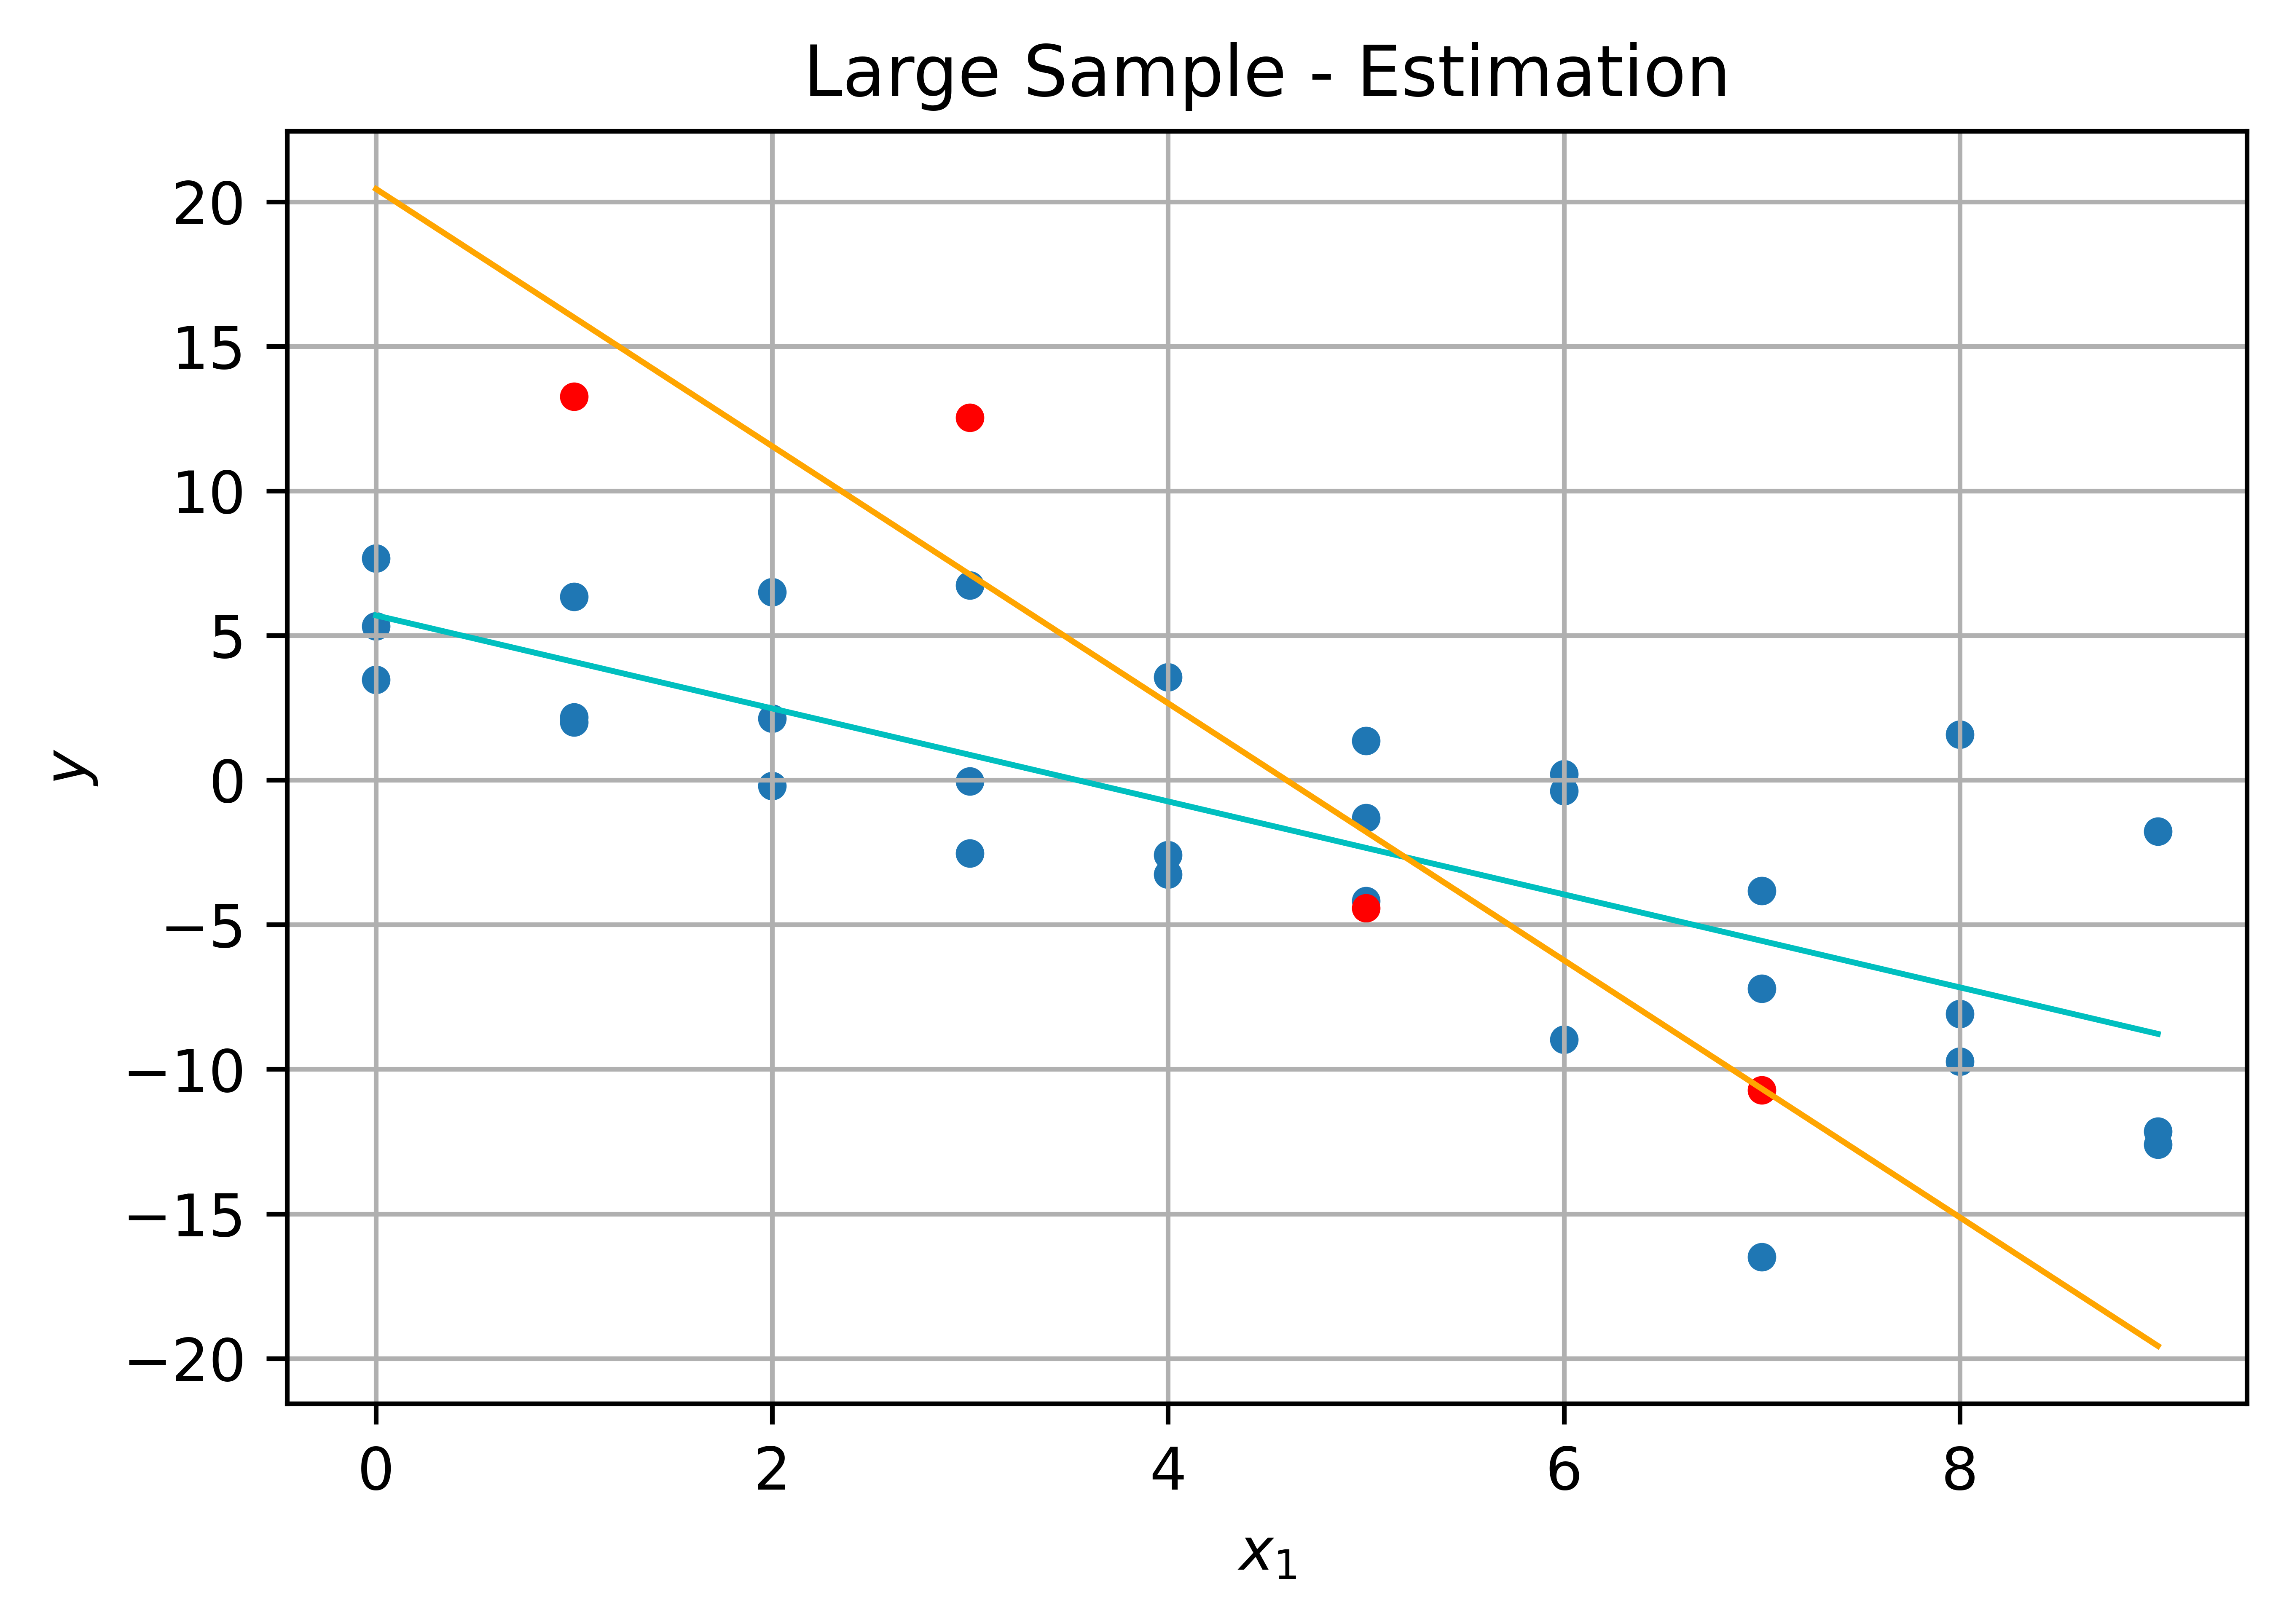
\includegraphics[width=70mm,scale=0.5]{images/regression_images/Estimation_Full_Sample_Regression.png}
        
            \caption*{Our regression from before doesn't look so good on this model... We make an updated regression, and get a more accurate result.}
        \end{figure}
        
        \begin{clarification}
           $\lambda$ doesn't lower \purp{estimation error} in the \gren{same way} that increasing \purp{sample size} does, but the problem is \gren{similar}.
        \end{clarification}
        
    \subsection{Tradeoffs: Structural Error}
    
        However, not all problems are caused by estimation error: sometimes, it \textbf{isn't even possible} to get a good result - you chose the wrong \textbf{model class}.
        
        This means the \textbf{structure} of your model is the problem, not your method of \textbf{estimation}. Thus, we call this \vocab{structural error}.\\
        
        \begin{definition}
            \vocab{Structural error} is the error that results from having the wrong \gren{structure} for the \purp{task} you are trying to accomplish.
            
            This can result from the \gren{wrong class} of model, but sometimes, your model class doesn't have the \purp{expressiveness} it needs for a complex problem.
            
            It can also happen if your algorithm \purp{limits} the available models in some way, like how $\lambda$ does.
        \end{definition}
        
        \miniex If the \textbf{true shape} of a distribution is a parabola $x^2$, there is \textbf{no} linear function $mx+b$ that can match that: this creates \textbf{structural error}.
        
        \begin{figure}[H]
        
                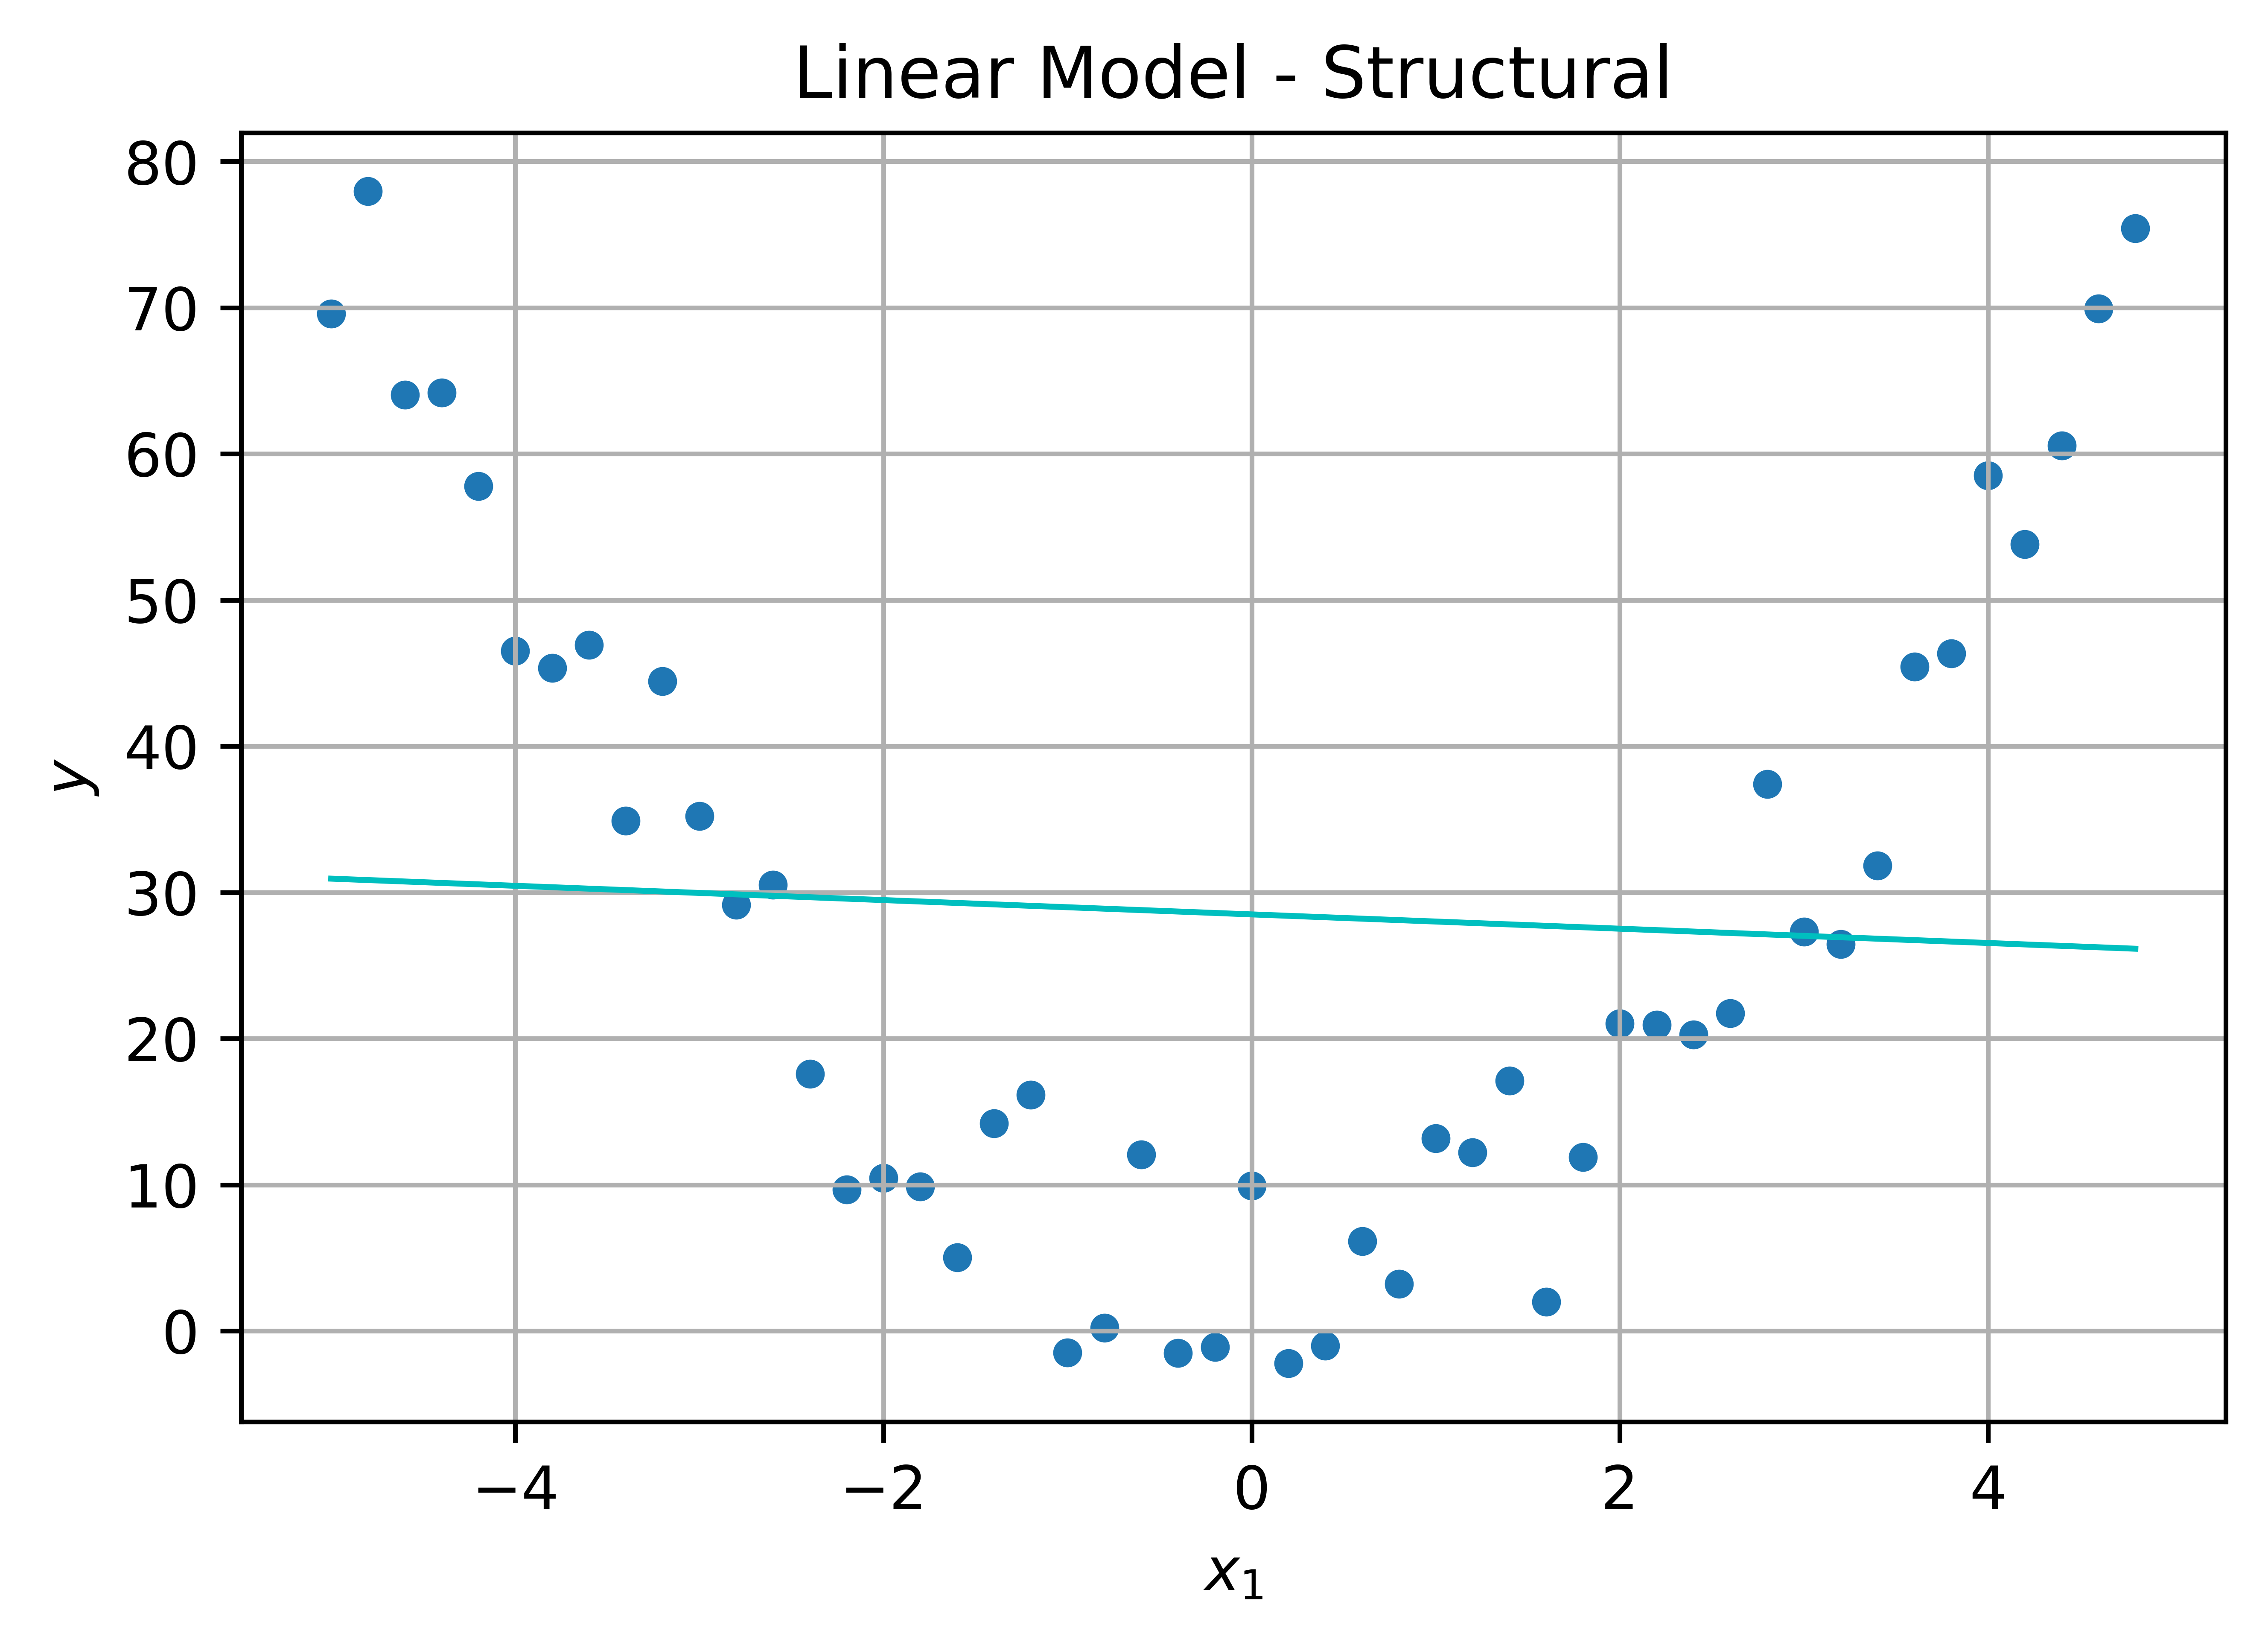
\includegraphics[width=70mm,scale=0.5]{images/regression_images/Structural_Linear_Model.png}

                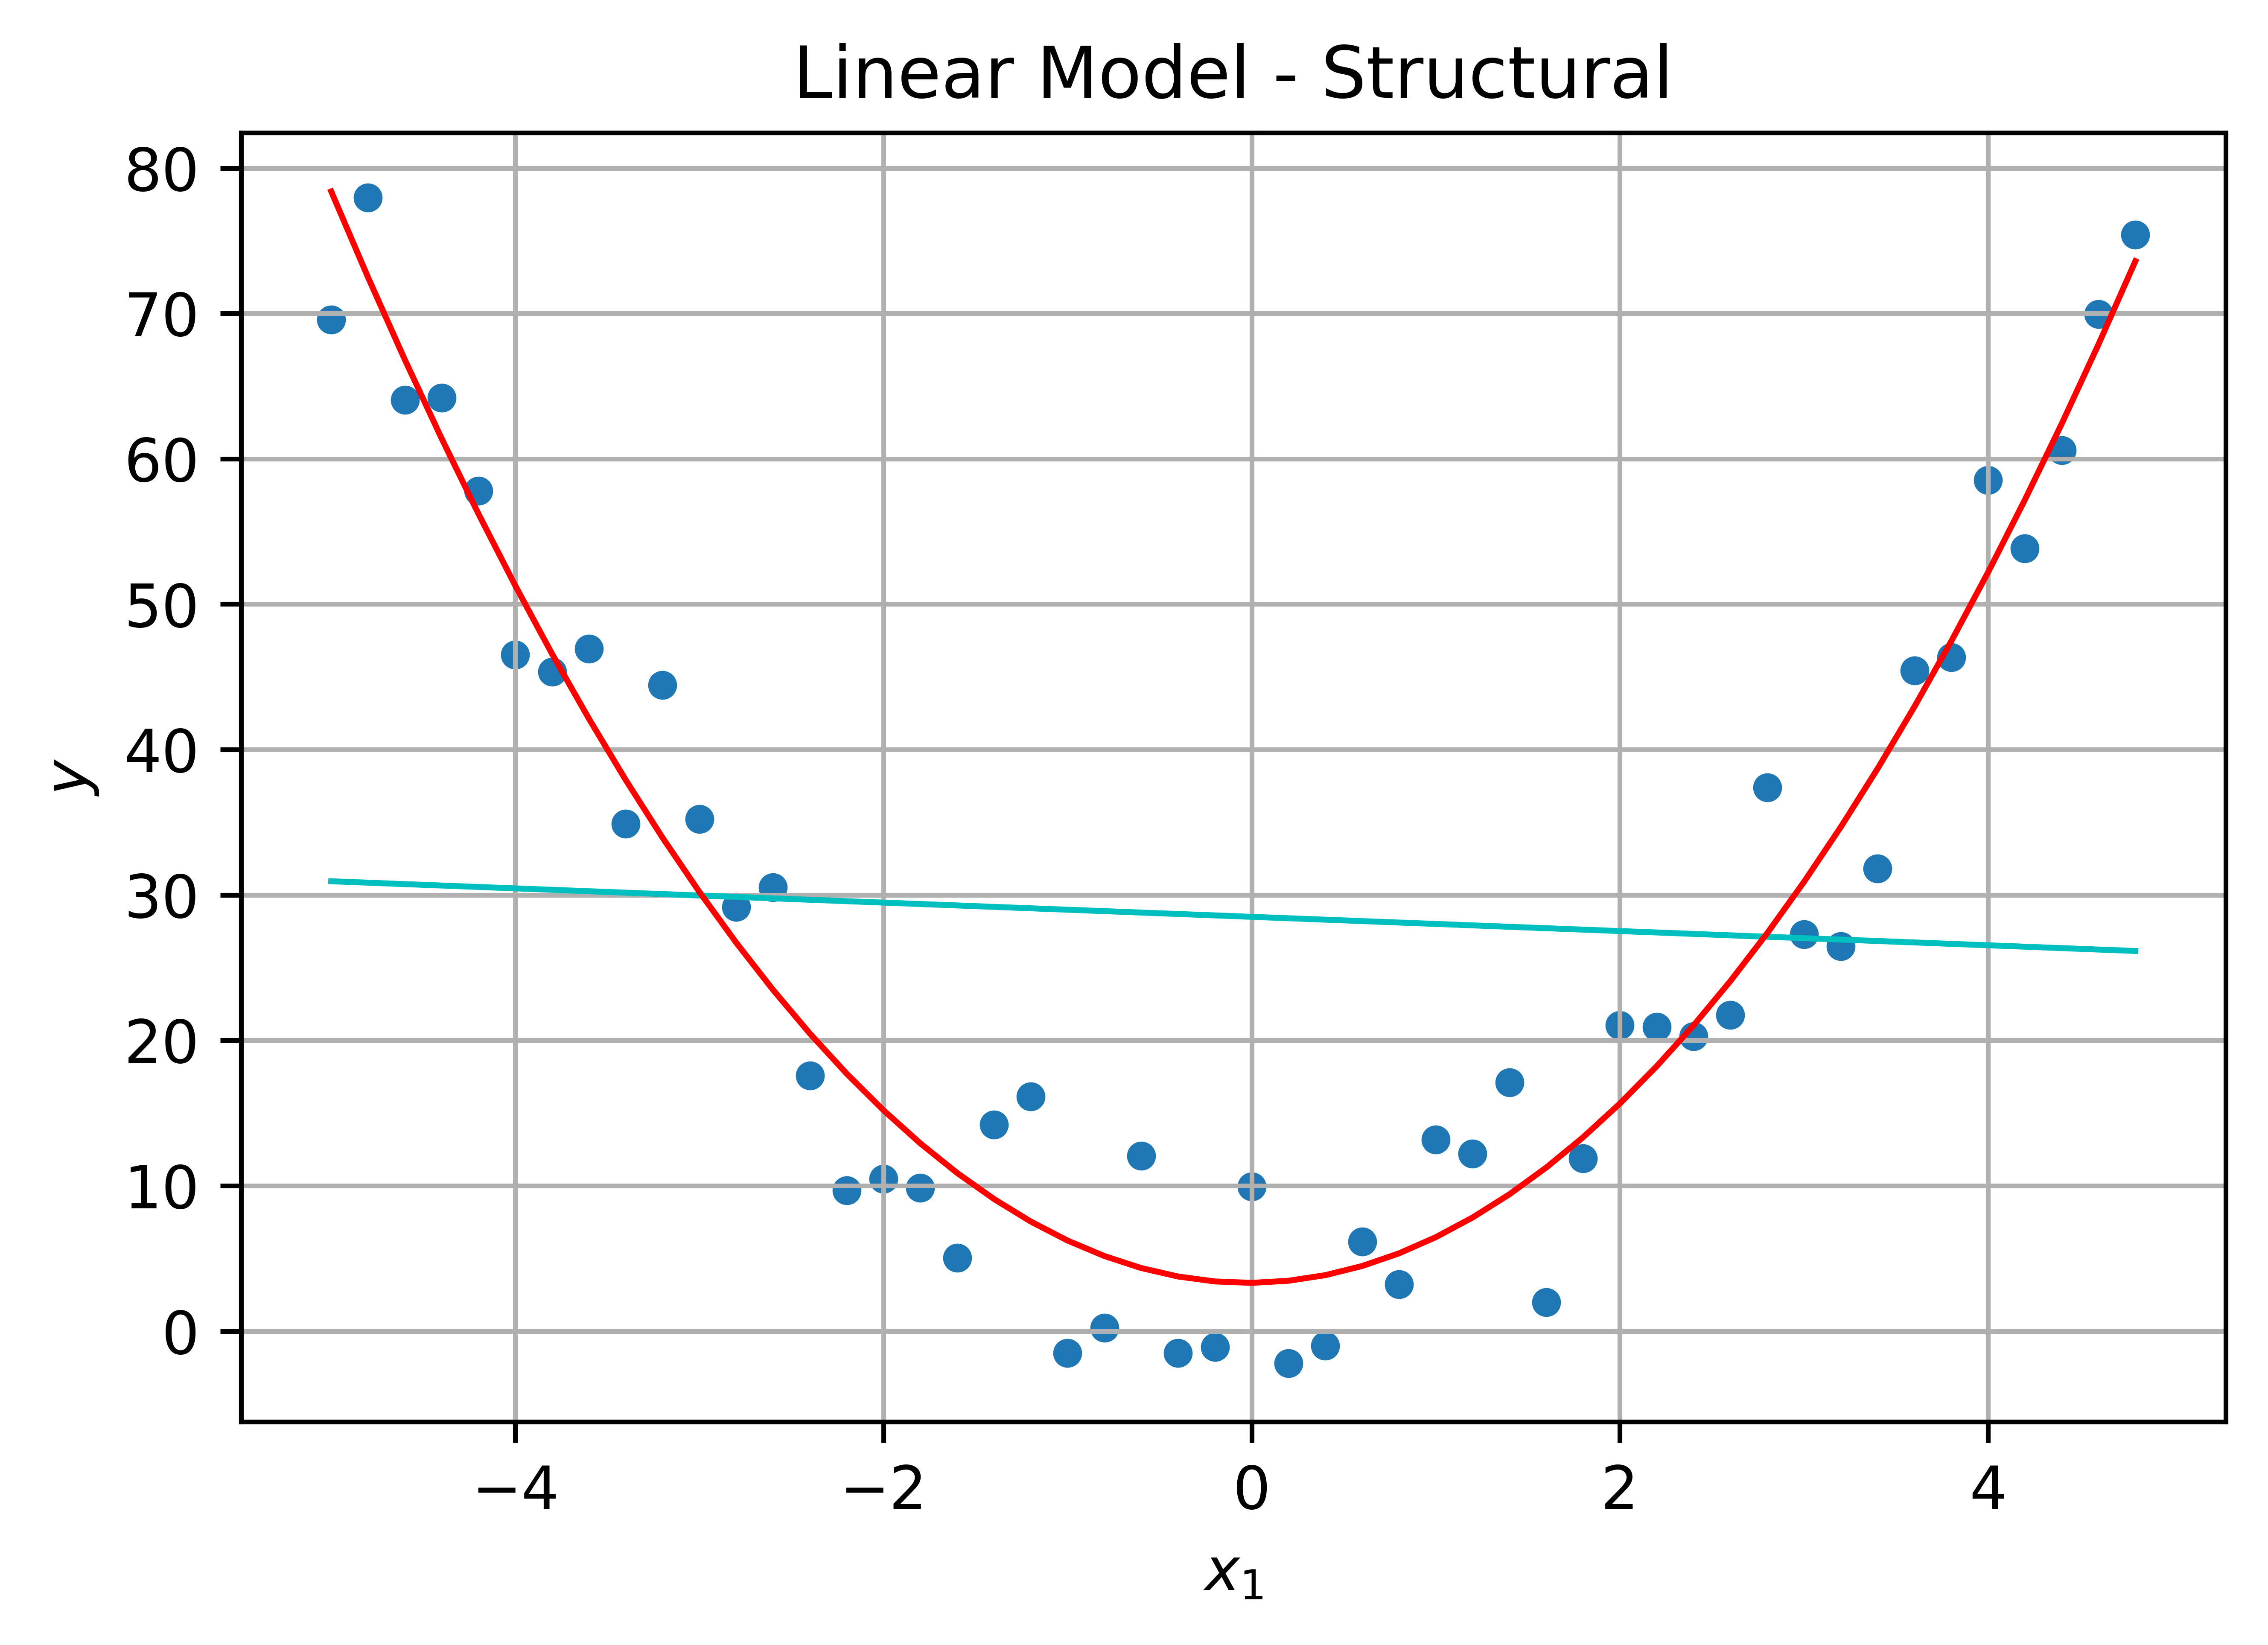
\includegraphics[width=70mm,scale=0.5]{images/regression_images/Structural_Quad_Model.png}

        
            \caption*{Our \textbf{linear} model isn't able to represent a quadratic function... so, we switch to a more \textbf{expressive} model: a \textbf{quadratic} equation.}
        \end{figure}
        
        \note{Remember that \textbf{expressiveness} is about how many possible models you have: if you have more models, you can solve more problems.}
        
        \begin{clarification}
           Note that $\lambda$ does not restrict our model class \purp{as severely} as \gren{switching polynomial order}, like above. 
        
            But, $\lambda$ \purp{limits} the use of larger $\theta$, which does make it \gren{unable} to solve some problems. So, the \purp{structural error} problem is similar.
        \end{clarification}
        
    \subsection{Tradeoffs of $\lambda$}
        
        Based on these two categories, we can discuss the tradeoffs of $\lambda$ more easily.
        
        As we mentioned, regularization \textbf{reduces} estimation error: 
        
        If we overfit to our current data, we are poorly \textbf{estimating} the distribution, because the training data may not perfectly \textbf{represent} it.\\
        
        \begin{concept}
            A \vocab{large $\lambda$} means \purp{more regularization}: we more strongly push for a more \gren{general} model, over a more \gren{specific} one.
            
            This results in...
            
            \begin{itemize}
                \item \gren{Reduced} estimation error
                \item \purp{Increased} structural error
            \end{itemize}
        \end{concept}
        
        However, \textbf{regularization} also \textbf{limits} the possible models we can use - those it views as less "general", it \textbf{penalizes}.

        \begin{itemize}
            \item That means the scope of possible models is \textbf{smaller} - some models are no longer \textbf{acceptable}. What if the only valid solution was in that space we \textbf{restricted}? Well, then we can't \textbf{find} it.
            
            \item That means there are certain \textbf{structural} limits on our model: that means that regularization \textbf{increases} structural error!\\
        \end{itemize}
        
        
        
        
        
        \begin{concept}
            A \vocab{small $\lambda$} means \purp{less regularization}: we care less about a more \gren{general} model, allowing more \gren{specific} data to come into play.
            
            This results in...
            
            \begin{itemize}
                \item \purp{Increased} estimation error
                \item  \gren{Reduced} structural error
            \end{itemize}
        \end{concept}
        
    \subsection{Evaluating Hypotheses}
    
        So, we know that we have these \textbf{two} types of \textbf{error}. But it's \textbf{difficult} to \textbf{measure} them separately. 
        
        So instead, we just want to measure the \textbf{overall performance} of our hypothesis. 
        
        We do this using our \textbf{testing error}: this tells us how good our hypothesis is \textbf{after} training.
        
        \begin{equation}
            \testerr(h) =
            \frac{1}{m}  
            \sum_{i\purp{=n+1}}^{\purp{n+m}} 
                \left( 
                    h(\ex{x}{i}) - \ex{y}{i} 
                \right)^2
        \end{equation}
        
        Note that, before, we were using \textbf{regularization}. This is so we can \textbf{make} a more \textbf{general} model. 
        
        But here, we've \textbf{removed} it, because training is \textbf{done}: we're \textbf{not} going to make our hypothesis \textbf{better}. We just care about how \textbf{good} it came out.
        \note{We're already measuring the \textbf{generalizability} by using \textbf{new data}!}\\
        
        \begin{clarification}
            When we \vocab{evaluate a hypothesis} using \purp{testing error}, we are \gren{done training}: our hypothesis will not change.
            
            Because of this, we \orgg{do not} include the \orgg{regularizer} when \gren{evaluating} our hypothesis.
        \end{clarification}
        
    \subsection{$\lambda$'s purpose: learning algorithms}
    
        Notice that we \textbf{removed} regularization when we were \textbf{evaluating} our hypothesis: regularization was used to \textbf{create} our hypothesis, but it is not \textbf{part} of that hypothesis.
        \note{Our hypothesis only includes the parameters $\Theta$: not $\lambda$!}
        
        That's because $\lambda$ is part of our \textbf{algorithm}: it determines how we find our hypothesis. So, let's talk about that.\\
        
        \begin{definition}
            A \vocab{learning algorithm} is our procedure for \purp{learning} from data. It uses that data to create a \gren{hypothesis}. We can diagram this as:
            
            \begin{equation*}
                \data_n \longrightarrow 
                \boxed{\text{learning alg ($\hclass$)}} 
                \longrightarrow h
            \end{equation*}
            
            In a way, it's a function that takes in \gren{data} $\data_n$, and outputs a \purp{hypothesis} $h$.
        \end{definition}
        
        We're choosing \textbf{one hypothesis} $h$ from the hypothesis class $\hclass$: this is why $\hclass$ appears in the notation above.
        \note{We can write this as $h \in \hclass$}
        
    \subsection{Comparing Hypotheses and Learning Algorithms}
        
        We can take our learning algorithm
        
        \begin{equation*}
            \data_n \longrightarrow 
            \boxed{\text{learning alg ($\hclass$)}} 
            \longrightarrow h
        \end{equation*}
        
        And compare it to our hypothesis $h$:
        
        $$ x \rightarrow \boxed{h} \rightarrow y $$
        
        In a way, our learning algorithm is a function, that outputs another function!
        \note{This is similar to $\trainerr$, which instead takes a function as \textbf{output}!}

        \begin{itemize}
            \item Our \gren{hypothesis} can be adjusted with our \purp{parameter} $\Theta$: if we change $\Theta$, we change our \textbf{performance}.
            
            \item Our \gren{learning algorithm} depends on $\lambda$: so, $\lambda$ is like a \purp{parameter}. But, it's different from $\Theta$: $\Theta$ \orgg{is} our model, $\lambda$ controls how we \orgg{choose} our model.
                \begin{itemize}
                    \item So, it's a parameter ($\lambda$) that affects other parameters ($\Theta$). Because of that, we call it a \textbf{hyperparameter}.
                        \note{It affects our hypothesis by pressuring it to have lower magnitude!}\\
                \end{itemize}
        \end{itemize}
        
        
        
        
        
        
        
        \begin{definition}
            \purp{Parameters} are \gren{variables} that adjust the behavior of \purp{our model}: our hypothesis.
            
            A \vocab{hyperparameter} is a \gren{variable} that can adjust \purp{how we make models}: our learning algorithm. 
        \end{definition}
        
        The \textbf{only} hyperparameter we have for now is $\lambda$, but the \textbf{development} of hyperparameters is an ongoing area of \textbf{research}.\\
        
        \begin{concept}
            \vocab{Lambda}, or $\lambda$, is a \vocab{hyperparameter}: it controls our \purp{learning algorithm.}
        \end{concept}
        
    \subsection{Evaluating our Learning Algorithm}
    
        So, while we can evaluate each \textbf{hypothesis}, it's also important to measure how our \textbf{learning algorithm} is performing.
        
        How do we measure it? Well, the job of our \textbf{learning algorithm} is to \textbf{pick good hypotheses}.\\
        
        \begin{concept}
            We can \vocab{evaluate} the performance of a \vocab{learning algorithm} using \orgg{testing loss}: a good learning algorithm will create \gren{hypotheses} with low testing loss.
        \end{concept}
        
        You could think of this as measuring the \textbf{skill} of a \textbf{teacher} (the learning algorithm) by the \textbf{success} of their \textbf{student} (the hypothesis) on a \textbf{test} (testing loss).
        
    \subsection{Validation: Evaluating with lots of data}
    
        When we were creating hypotheses, \purp{randomness} caused some problems: you might not get \textbf{training data} that matched the \textbf{testing data} very well.
        
        The \textbf{same} can happen here, when \textbf{evaluating} your \textbf{algorithm}: maybe your model happened to create a bad (or unusually good!) hypothesis because of \textbf{luck}.
        
        The easy solution to \textbf{randomness} is to add \gren{more data}: we get more \textbf{consistency} that way.
        
        So, we \textbf{repeatedly} get new training data and test data. For each, we train a \orgg{different hypothesis}. We can \textbf{average} their performance out, and use that to \textbf{estimate} the quality of our algorithm.\\
        
        \begin{definition}
            \vocab{Validation} is a way to \vocab{evaluate a learning algorithm} using \vocab{large amounts of data}.
            
            We do this by \gren{running} our algorithm \purp{many times} with new data, and \gren{averaging} the testing error of all the hypotheses.

            \begin{itemize}
                \item This process is often requires having \purp{lots of data} to train with, but is a \textbf{provably} good approach.
            \end{itemize}
            
        \end{definition}
        
    \subsection{Our Problem: When data is less available}
        
        As mentioned, this takes up \textbf{lots of data}. What if our data is limited?
            \note{Data is often \textbf{expensive}. It might even be impossible to get more!}

        In this case, we'll assume that have some \textbf{finite} data, $\data_n$. We \textbf{can't get more}.
        
        Previously, we solved validation by using \textbf{more data}, and generating \gren{multiple hypotheses}.

        \begin{itemize}
            \item One set of data gives us one \textbf{hypothesis}.

            \item But, what if, rather than using \textbf{completely} new data for each hypothesis, we used \orgg{slightly different} data each time?
        \end{itemize}
        
         
        
        First, need to break $\data_n$ into a chunk for training, and a chunk for testing.
        
        \begin{figure}[H]
        \centering
            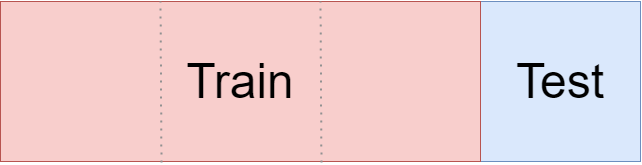
\includegraphics[width=70mm,scale=0.5]{images/regression_images/training_and_test_data.png}
        \end{figure}
        
        How do we get more hypotheses from this dataset?
        
    \subsection{Cross-Validation}
    
        We mentioned that we want \textbf{different} hypotheses. Our hypotheses depend on our \textbf{training data}. So we want to \textbf{change} our training data.
        
        We can't \textbf{add} data to it, because then we \textbf{lose} testing data. We shouldn't \textbf{remove} training data, because then we're just making a hypothesis that's \textbf{less well-informed}.
        
        Instead, we'll \textbf{swap} some of the training data for testing data.
        
        \begin{figure}[H]
        \centering
            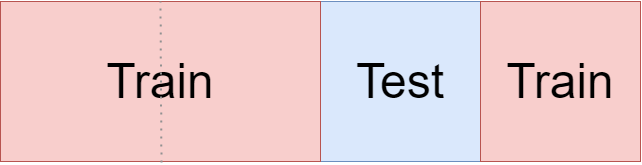
\includegraphics[width=70mm,scale=0.5]{images/regression_images/training_and_test_data_2.png}
        \end{figure}
        
        This will create a new hypothesis, and the data is partially different! In fact, we can do this for each of our chunks:
        
        \begin{figure}[H]
                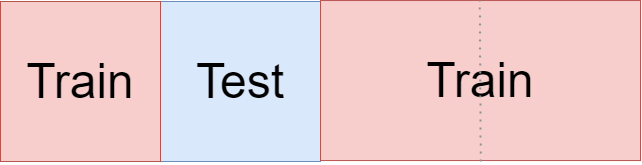
\includegraphics[width=70mm,scale=0.5]{images/regression_images/training_and_test_data_3.png}
                
                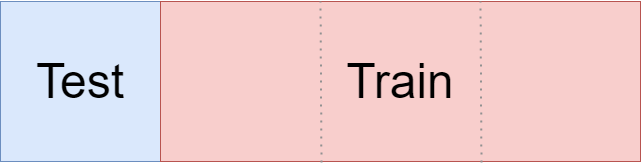
\includegraphics[width=70mm,scale=0.5]{images/regression_images/training_and_test_data_4.png}
            
        \end{figure}
        
        We now have \textbf{four different hypotheses} for the price of one!\\
        
        \begin{definition}
            \vocab{Cross-validation} is a way to \gren{evaluate} a learning algorithm using \purp{limited data}.

            \begin{itemize}
                \item We do this by \purp{breaking} our data it into \gren{chunks} to create \orgg{multiple hypotheses} from one dataset.
                
                \item For each \gren{chunk}, we train one dataset on all the data \orgg{not in that chunk}. We get our \purp{test error} using the chunk \textbf{we left out}.
            \end{itemize}
            
            For $k$ chunks, we end up with $k$ hypotheses. By \gren{averaging} out their performance, we can \purp{approximate} the quality of our algorithm.
        \end{definition}
        
        This approach is much \textbf{less expensive}, and very common in machine learning! 
            \note{But, some of the theoretical \textbf{benefits} of validation are not \textbf{proven} to be true for cross-validation.}\\
        
        \begin{clarification}
            Note that the goal of validation and cross-validation is \textbf{not} to evaluate \purp{one hypothesis}.
            
            Instead, it is instead meant to evaluate a \purp{learning algorithm}. This is why we have to create \purp{many} hypotheses: we want to see that our algorithm is \gren{generally} good!
        \end{clarification}
        
    \subsection{Hyperparameter Tuning}
    
        Now, we know how to \textbf{evaluate} a learning algorithm, just like how we \textbf{evaluate} a hypothesis. 
        
        Once we knew how to evaluate a hypothesis, we started optimizing our \gren{parameters} for the \textbf{best} hypothesis. So, we could do the same for our \textbf{learning algorithm}.

        How do we \orgg{optimize} a learning algorithm?
        
        Each $\lambda$ value creates a slightly \textbf{different} learning algorithm: we can \textbf{optimize} this \textbf{hyperparameter} to create the \textbf{best} learning algorithm.
        
    \subsection{How to tune our algorithm}
    
        When we were \textbf{optimizing} our hypothesis, we started by \textbf{randomly} trying hypotheses. Then, we used an \textbf{analytical} approach.
        \note{By "analytical", we mean directly creating an equation, and solving it.}
        
        We don't always have \textbf{simple} equations to work with: with all of our data, it's hard to come up with \textbf{manageable} equations. So, we \textbf{won't} try doing it \textbf{analytically}.
        
        So, we could \textbf{randomly} try $\lambda$ values and pick the \textbf{best} one. This is pretty \textbf{close} to what we usually end up doing. For each value we pick, we'll use \gren{cross-validation} to evaluate.
        
        For now, we'll systematically go through $\lambda$ values: $\lambda=.1, .2, .3 \dots$\\
        
        \begin{concept}
            \vocab{Hyperparameter tuning} is how we \purp{optimize} our \gren{learning algorithm} to create the \purp{best} hypotheses.
            
            The simplest way to do this is to try \gren{multiple} different values of $\lambda$. For each value, we use \gren{cross-validation} to evaluate that learning algorithm.
            
            Finally, we pick whichever $\lambda$ gives you the \purp{best} algorithm, and thus the \purp{best} hypotheses.
        \end{concept}
        
    \subsection{Hyperparameter Tuning: Two kinds of optimization}
    
        There's something often \textbf{confusing} about hyperparameter tuning to students:
            \note{In case the word "optimization" starts to look like gibberish in this section, remember: it just means, "find the best option".}

        \begin{itemize}
            \item When we're \textbf{optimizing} $\lambda$, we try many values $\lambda_j$. Each $\lambda_j$ create a \purp{learning algorithm} we have to evaluate. 
            
            \item But a single learning algorithm is already an optimization problem: the learning algorithm is supposed to find $\Theta$.

                \begin{itemize}
                    \item So, we have to \orgg{optimize} $\Theta$, while we're in the middle optimizing $\lambda$.
                \end{itemize}
        \end{itemize}
        
        
        That means, \textbf{every time} we try a different $\lambda$ value, we have to do one optimization problem. Optimizing $\Theta$ many times, lets you optimize $\lambda$ once.
            \note{Remember that, in this situation, $\Theta$ and $h$ are almost(but not quite) the same thing.}

        \begin{equation*}
                \begin{rcases}
                \begin{matrix}
                    \data_n \longrightarrow 
                    \boxed{\text{learn alg using $\red{\lambda_1}$}} 
                    \longrightarrow \Theta_1
                    \longrightarrow
                    \boxed{\text{Test error }}
                    \longrightarrow 
                    \overbrace{\testerr(h_1)} ^{\text{Evaluates }\red{\lambda_1}} \\\\
                    \data_n \longrightarrow 
                    \boxed{\text{learn alg using $\red{\lambda_2}$}} 
                    \longrightarrow \Theta_2
                    \longrightarrow
                    \boxed{\text{Test error }}
                    \longrightarrow 
                    \overbrace{\testerr(h_2)} ^{\text{Evaluates }\red{\lambda_2}} \\
                    \vdots \\
                    \data_n \longrightarrow 
                    \boxed{\text{learn alg using $\red{\lambda_n}$}} 
                    \longrightarrow \Theta_n
                    \longrightarrow
                    \boxed{\text{Test error }}
                    \longrightarrow 
                    \overbrace{\testerr(h_n)} ^{\text{Evaluates }\red{\lambda_n}}
                \end{matrix}
                \end{rcases}\text{Pick best $\lambda_j$ using $\testerr$}  
            \end{equation*}
        
        That means we have \textbf{two layers} of optimization!\\
        
        \begin{clarification}
            We \purp{optimize} $\lambda$ by trying many values.

            \begin{itemize}
                \item But, for each $\lambda$ value, we have to \gren{optimize} $\Theta$.
            \end{itemize}
            
            So, we have to optimize $\Theta$ \purp{repeatedly} in order to optimize $\lambda$ \purp{once}! This gives us $\lambda^*.$
        \end{clarification}
        
        Once we've found our best hyperparameter $\lambda^*$, we can use it to get our best parameters: $\theta^*$.
        
    \subsection{Pseudocode Example}
        
        This technique is \textbf{not} limited to regression. Thus, we'll be a bit more \textbf{general}: we won't assume an \textbf{analytical} solution. Instead, we \textbf{optimize} by just trying different $\Theta$ values.
        
        We can represent this in pseudocode:
        \note{If this pseudocode isn't helpful to you, don't worry! Some students like it, some don't.}
        
        \begin{codebox}
            \Procname{$\proc{Lambda-Optimization}
                       (\data, lambda\_values, theta\_values)$}
                       
                \li \For $\lambda$ \In $lambda\_values$        
                \qquad\quad\#Try lambda values
                
                \li     \Do \For $\Theta$ \In $theta\_values$  
                \qquad\quad\#Try theta values    
                            \Do

                                \li Calculate $J(\Theta)$    
                                \qquad\qquad\qquad\#Compare values
                            \End
                        
                        \li Choose best theta value $\Theta^*$ 
                        \quad\#Best for each lambda

                        \End
                \li Choose best lambda value $\lambda^*$
                \li
                    
                \li \Return $\lambda^*$
        \end{codebox}
        
    To reiterate: this $\lambda^*$ will then we used to get our final result, $\theta^*$.

\pagebreak
        
\section{Terms}

    \begin{itemize}
        \item Hypothesis
        \item Theta ($\Theta$)
        \item Input Space
        \item Regression
        \item Feature
        \item Feature Transformation
        \item Training Error
        \item Test Error
        \item Objective Function
        \item Min function
        \item Argmin function
        \item Star Notation ($\theta^*$)
        \item Linear Regression
        \item Hypothesis Class
        \item Square Loss
        \item Ordinary Least Squares (OLS) Problem
        \item OLS Objective Function
        \item Hyperplane
        \item Weight
        \item Input Matrix
        \item Output Matrix
        \item Gradient
        \item OLS Solution
        \item Regularization
        \item Regularizer
        \item Regularizer for Regression
        \item Lambda ($\lambda$)
        \item Ridge Regression
        \item RR Objective Function
        \item RR Solution
        \item Invertibility
        \item Estimation Error
        \item Structural Error
        \item Expressiveness
        \item Learning Algorithm
        \item Hyperparameter
        \item Validation
        \item Cross-Validation
        \item Chunk (Cross-Validation)
        \item Hyperparameter Tuning
    \end{itemize}
        
        
        






%%% Local Variables:
%%% mode: latex
%%% TeX-master: "top"
%%% End:
